% Options for packages loaded elsewhere
\PassOptionsToPackage{unicode}{hyperref}
\PassOptionsToPackage{hyphens}{url}
%
\documentclass[
  11pt,
]{article}
\usepackage{lmodern}
\usepackage{amssymb,amsmath}
\usepackage{ifxetex,ifluatex}
\ifnum 0\ifxetex 1\fi\ifluatex 1\fi=0 % if pdftex
  \usepackage[T1]{fontenc}
  \usepackage[utf8]{inputenc}
  \usepackage{textcomp} % provide euro and other symbols
\else % if luatex or xetex
  \usepackage{unicode-math}
  \defaultfontfeatures{Scale=MatchLowercase}
  \defaultfontfeatures[\rmfamily]{Ligatures=TeX,Scale=1}
\fi
% Use upquote if available, for straight quotes in verbatim environments
\IfFileExists{upquote.sty}{\usepackage{upquote}}{}
\IfFileExists{microtype.sty}{% use microtype if available
  \usepackage[]{microtype}
  \UseMicrotypeSet[protrusion]{basicmath} % disable protrusion for tt fonts
}{}
\makeatletter
\@ifundefined{KOMAClassName}{% if non-KOMA class
  \IfFileExists{parskip.sty}{%
    \usepackage{parskip}
  }{% else
    \setlength{\parindent}{0pt}
    \setlength{\parskip}{6pt plus 2pt minus 1pt}}
}{% if KOMA class
  \KOMAoptions{parskip=half}}
\makeatother
\usepackage{xcolor}
\IfFileExists{xurl.sty}{\usepackage{xurl}}{} % add URL line breaks if available
\IfFileExists{bookmark.sty}{\usepackage{bookmark}}{\usepackage{hyperref}}
\hypersetup{
  hidelinks,
  pdfcreator={LaTeX via pandoc}}
\urlstyle{same} % disable monospaced font for URLs
\usepackage[margin=1in]{geometry}
\usepackage{color}
\usepackage{fancyvrb}
\newcommand{\VerbBar}{|}
\newcommand{\VERB}{\Verb[commandchars=\\\{\}]}
\DefineVerbatimEnvironment{Highlighting}{Verbatim}{commandchars=\\\{\}}
% Add ',fontsize=\small' for more characters per line
\newenvironment{Shaded}{}{}
\newcommand{\AlertTok}[1]{\textcolor[rgb]{1.00,0.00,0.00}{\textbf{#1}}}
\newcommand{\AnnotationTok}[1]{\textcolor[rgb]{0.38,0.63,0.69}{\textbf{\textit{#1}}}}
\newcommand{\AttributeTok}[1]{\textcolor[rgb]{0.49,0.56,0.16}{#1}}
\newcommand{\BaseNTok}[1]{\textcolor[rgb]{0.25,0.63,0.44}{#1}}
\newcommand{\BuiltInTok}[1]{#1}
\newcommand{\CharTok}[1]{\textcolor[rgb]{0.25,0.44,0.63}{#1}}
\newcommand{\CommentTok}[1]{\textcolor[rgb]{0.38,0.63,0.69}{\textit{#1}}}
\newcommand{\CommentVarTok}[1]{\textcolor[rgb]{0.38,0.63,0.69}{\textbf{\textit{#1}}}}
\newcommand{\ConstantTok}[1]{\textcolor[rgb]{0.53,0.00,0.00}{#1}}
\newcommand{\ControlFlowTok}[1]{\textcolor[rgb]{0.00,0.44,0.13}{\textbf{#1}}}
\newcommand{\DataTypeTok}[1]{\textcolor[rgb]{0.56,0.13,0.00}{#1}}
\newcommand{\DecValTok}[1]{\textcolor[rgb]{0.25,0.63,0.44}{#1}}
\newcommand{\DocumentationTok}[1]{\textcolor[rgb]{0.73,0.13,0.13}{\textit{#1}}}
\newcommand{\ErrorTok}[1]{\textcolor[rgb]{1.00,0.00,0.00}{\textbf{#1}}}
\newcommand{\ExtensionTok}[1]{#1}
\newcommand{\FloatTok}[1]{\textcolor[rgb]{0.25,0.63,0.44}{#1}}
\newcommand{\FunctionTok}[1]{\textcolor[rgb]{0.02,0.16,0.49}{#1}}
\newcommand{\ImportTok}[1]{#1}
\newcommand{\InformationTok}[1]{\textcolor[rgb]{0.38,0.63,0.69}{\textbf{\textit{#1}}}}
\newcommand{\KeywordTok}[1]{\textcolor[rgb]{0.00,0.44,0.13}{\textbf{#1}}}
\newcommand{\NormalTok}[1]{#1}
\newcommand{\OperatorTok}[1]{\textcolor[rgb]{0.40,0.40,0.40}{#1}}
\newcommand{\OtherTok}[1]{\textcolor[rgb]{0.00,0.44,0.13}{#1}}
\newcommand{\PreprocessorTok}[1]{\textcolor[rgb]{0.74,0.48,0.00}{#1}}
\newcommand{\RegionMarkerTok}[1]{#1}
\newcommand{\SpecialCharTok}[1]{\textcolor[rgb]{0.25,0.44,0.63}{#1}}
\newcommand{\SpecialStringTok}[1]{\textcolor[rgb]{0.73,0.40,0.53}{#1}}
\newcommand{\StringTok}[1]{\textcolor[rgb]{0.25,0.44,0.63}{#1}}
\newcommand{\VariableTok}[1]{\textcolor[rgb]{0.10,0.09,0.49}{#1}}
\newcommand{\VerbatimStringTok}[1]{\textcolor[rgb]{0.25,0.44,0.63}{#1}}
\newcommand{\WarningTok}[1]{\textcolor[rgb]{0.38,0.63,0.69}{\textbf{\textit{#1}}}}
\usepackage{longtable,booktabs}
% Correct order of tables after \paragraph or \subparagraph
\usepackage{etoolbox}
\makeatletter
\patchcmd\longtable{\par}{\if@noskipsec\mbox{}\fi\par}{}{}
\makeatother
% Allow footnotes in longtable head/foot
\IfFileExists{footnotehyper.sty}{\usepackage{footnotehyper}}{\usepackage{footnote}}
\makesavenoteenv{longtable}
\usepackage{graphicx}
\makeatletter
\def\maxwidth{\ifdim\Gin@nat@width>\linewidth\linewidth\else\Gin@nat@width\fi}
\def\maxheight{\ifdim\Gin@nat@height>\textheight\textheight\else\Gin@nat@height\fi}
\makeatother
% Scale images if necessary, so that they will not overflow the page
% margins by default, and it is still possible to overwrite the defaults
% using explicit options in \includegraphics[width, height, ...]{}
\setkeys{Gin}{width=\maxwidth,height=\maxheight,keepaspectratio}
% Set default figure placement to htbp
\makeatletter
\def\fps@figure{htbp}
\makeatother
\setlength{\emergencystretch}{3em} % prevent overfull lines
\providecommand{\tightlist}{%
  \setlength{\itemsep}{0pt}\setlength{\parskip}{0pt}}
\setcounter{secnumdepth}{-\maxdimen} % remove section numbering
\usepackage{amssymb}
\usepackage{pifont}
\usepackage{fvextra}
% wrap long lines in pandoc's highlighted code blocks (the prompt docstrings)
\fvset{breaklines=true,breakanywhere=true}
\usepackage{etoolbox}
% Heated tables/captions use a sans face loaded from the .otf files bundled in fonts/, by path
% rather than by system name — bundling the files keeps arXiv's scanner from flagging the font
% as a missing source file, and guarantees the same sharp sans on their TeX Live.
\usepackage{fontspec}
% Body fonts loaded by PATH from the bundled .ttf files (not by system name), so arXiv's
% scanner sees source files rather than missing system fonts ("DejaVu Serif"/"DejaVu Sans").
\setmainfont[Path=fonts/, BoldFont=DejaVuSerif-Bold.ttf, ItalicFont=DejaVuSerif-Italic.ttf,
  BoldItalicFont=DejaVuSerif-BoldItalic.ttf]{DejaVuSerif.ttf}
\setsansfont[Path=fonts/, BoldFont=DejaVuSans-Bold.ttf, ItalicFont=DejaVuSans-Oblique.ttf,
  BoldItalicFont=DejaVuSans-BoldOblique.ttf]{DejaVuSans.ttf}
\newfontfamily\tablefont[Ligatures=TeX, Path=fonts/,
  BoldFont=texgyreheros-bold.otf, ItalicFont=texgyreheros-italic.otf,
  BoldItalicFont=texgyreheros-bolditalic.otf]{texgyreheros-regular.otf}
% Tables (longtable) in sans-serif, left-aligned so captions line up at the left margin.
\AtBeginEnvironment{longtable}{\tablefont\small\setlength{\tabcolsep}{4pt}}
% centre longtables (\fill on both sides), matching the centred heated/table floats.
\setlength{\LTleft}{\fill}
\setlength{\LTright}{\fill}
% Table caption/title (the "Table N." line above the table): sans-serif (TeX Gyre Heros,
% same as the table body), non-bold, LARGER than the 11pt body (13pt) so it reads as a title,
% left-aligned, indented from both sides (margin below). The footer note is styled smaller in
% build_arxiv.sh.
\usepackage{caption}
\usepackage{float}   % provides the [H] "exactly here" placement for the heated-table divs
\DeclareCaptionFont{tblcap}{\tablefont\fontsize{12}{14.5}\selectfont}
% figure captions: sans, footnotesize — the same size as a table's footer/note (not the larger table title)
\DeclareCaptionFont{tblnote}{\tablefont\footnotesize}
% margin=2.5em indents the title from both sides (an HTML-div-like block), so it does not
% run the full page width and is easy to tell apart from the body text.
\captionsetup{font=tblcap,labelfont=tblcap,labelsep=period,margin=2.5em,%
  justification=raggedright,singlelinecheck=false,skip=4pt}
% figure captions use the smaller table-note size (inherits margin/justification from above)
\captionsetup[figure]{font=tblnote,labelfont=tblnote}
% Keep floats near their text: let figures/tables fill more of a text page before
% LaTeX banishes them to a float-only page, so they land close to where they're cited.
\renewcommand{\topfraction}{0.92}
\renewcommand{\bottomfraction}{0.85}
\renewcommand{\textfraction}{0.06}
\renewcommand{\floatpagefraction}{0.78}
\setcounter{topnumber}{3}
\setcounter{totalnumber}{5}
% --- heattables (YlGnBu cell shading) ---
\usepackage{array}
\usepackage{colortbl}
\usepackage{tgheros}
\newcolumntype{H}{>{\centering\arraybackslash}m{1.05cm}}
\newcolumntype{B}{>{\raggedright\arraybackslash}m{3.0cm}}

\title{The Metanym Game: A Self-Contained, Self-Consistent LLM Peer-Community Benchmark for Structural Intelligence}
\author{David Nordfors (david.nordfors@archetypes.ai)}
\date{}

\begin{document}
\maketitle

\hypertarget{the-metanym-game-a-self-contained-self-consistent-llm-peer-community-benchmark-for-structural-intelligence}{%
\section{The Metanym Game: A Self-Contained, Self-Consistent LLM Peer-Community Benchmark for Structural Intelligence}\label{the-metanym-game-a-self-contained-self-consistent-llm-peer-community-benchmark-for-structural-intelligence}}

\hypertarget{abstract}{%
\subsection{Abstract}\label{abstract}}

The \emph{metanym game} is a competitive word game for LLMs that measures structural intelligence against established cognitive-science constructs. No content is given in advance; the contestants create all of it --- a new kind of analogy test, analogical \emph{production} falsifiable sentence by sentence, with no fixed test set to leak into training (contamination-resistant by construction). In the \emph{council-of-peers benchmark}, the contestants also rate each other's creations. We introduce the first spectral solution, to our knowledge, to the wicked problem of benchmarking LLMs' factual accuracy without golden keys or oracle models: one singular value decomposition of the evaluators' ratings matrix yields their competence as both generators and judges of true statements at once. Competence on the subjective criteria comes from each judge's rating consistency as the yardstick shifts. The factual rating correlates with GPQA Diamond at Pearson \(r = 0.92\). Scored separately, making and judging dissociate --- judging is the scarcer skill: the strongest generators are middling judges, the sharpest judge a mid-pack generator. To scale, the strongest players form a \emph{council} that does the official benchmarking; its seats are contestable --- a stronger model earns one on the benchmark's own rating. The benchmark is entirely self-contained and self-consistent, a stable gauge over time.

\begin{center}\rule{0.5\linewidth}{0.5pt}\end{center}

\hypertarget{introduction}{%
\subsection{1. Introduction}\label{introduction}}

Every benchmark for machine intelligence leans on an answer fixed in advance --- a gold label, a human rating, a reference solution. The benchmark reported here has none. Twelve frontier language models invent the test, sit it, and grade one another; the benchmark then works out which of them are competent to grade at all. No human raters, no answer key, nothing to look up.

The test is the \textbf{metanym game}. A player takes a paragraph describing one domain and turns it into a factually true description of an unrelated one by swapping a handful of words and leaving the rest untouched: a description of cell signalling becomes, swap by swap, a true description of human language, and then of a microservice architecture --- each sentence checkable on its own. The unchanged wording is a \emph{context template}, the swapped words are \emph{metanyms}, metaphorically synonymous, and each rewrite is a \emph{parallel context} of one underlying \emph{archetypal context}. The player chooses from no menu; it builds the structure from nothing. The metanym game makes a formal test of something a long tradition treats as central to thought --- seeing one structure across wildly different domains. Where that tradition tests whether you \emph{recognise} it, the game tests whether you can \emph{build} it, and checks the result sentence by sentence --- a new \emph{kind} of analogy test, not just a harder one.

Two properties follow from building the items this way. Because every item is produced fresh in the run, there is no fixed test set to leak into a later model's training data: the benchmark is contamination-resistant by construction (§3). And because correctness is settled sentence by sentence --- does this swapped claim hold in its new domain? --- the game needs no answer key. The models supply the verdicts themselves, and the benchmark reads the truth off their agreement: stack every model's true/false judgements into one matrix, and its dominant direction reveals which judges are competent, with no labels at all (§4.3, Appendix A). That competent subset becomes the \emph{council} that grades everyone --- a benchmark that certifies its own judges.

A single run then makes three things visible (§4). The twelve models split into a leading eight and a trailing four. The divide follows \emph{provider lineage} more than parameter count: one vendor's older generation falls away together with the roster's smallest seat, while within each family the size gradient is shallow. Judgement is the bottleneck: most models cannot reliably tell a true cross-domain claim from a false one, even when they produce competent structure themselves, so a model can be a perfectly \emph{consistent} grader and still a \emph{wrong} one. The strongest players --- the models that clear the reliability bar --- are seated as the council that issues the official ratings.

The game has a lineage --- in the cognitive science of analogy and structural mapping (§2), and in the systems-theory claim that one abstract structure can recur across unlike domains (von Bertalanffy 1968). The rest of the paper builds the game (§2), turns it into the self-administering council benchmark (§3), reports the canonical twelve-model run (§4), and weighs what the numbers do and do not license (§5).

\begin{center}\rule{0.5\linewidth}{0.5pt}\end{center}

\hypertarget{the-metanym-game}{%
\subsection{2. The metanym game}\label{the-metanym-game}}

This section presents the game, building it step-by-step and relating it to previous research on language and intelligence.

\hypertarget{a-the-context-template}{%
\subsubsection{2.a --- The context template}\label{a-the-context-template}}

Consider this passage describing \textbf{cell signalling}, from an old version of the Wikipedia article as it was worded when we first conceptualised the idea:

\begin{quote}
CELL SIGNALING is part of a complex system of communication that governs basic CELLULAR activities and coordinates CELL actions. The ability of CELLS to perceive and correctly respond to their MICROENVIRONMENT is the basis of development, TISSUE repair, and IMMUNITY as well as normal TISSUE HOMEOSTASIS. Errors in CELLULAR information processing are responsible for DISEASES. By understanding CELL SIGNALING, DISEASES may be treated effectively. SYSTEMS BIOLOGY research helps us to understand the underlying structure of CELL SIGNALING networks and how changes in these networks may affect the transmission and flow of information. CELL SIGNALING {[}is mostly thought of as{]} signaling between CELLS of a single ORGANISM. However, CELL SIGNALING may also occur between the CELLS of two different ORGANISMS. \emph{(adapted from Wikipedia's article on cell signalling)}
\end{quote}

Now substitute the set of marked keywords with another set:

\begin{quote}
HUMAN LANGUAGE is part of a complex system of communication that governs basic HUMAN activities and coordinates HUMAN actions. The ability of HUMANS to perceive and correctly respond to their ENVIRONMENT is the basis of development, COMMUNITY repair, and RESILIENCE as well as normal COMMUNITY EQUILIBRIUM. Errors in HUMAN information processing are responsible for DYSFUNCTIONS. By understanding HUMAN LANGUAGE, DYSFUNCTIONS may be treated effectively. SOCIOLOGY research helps us to understand the underlying structure of HUMAN LANGUAGE networks and how changes in these networks may affect the transmission and flow of information. HUMAN LANGUAGE {[}is mostly thought of as{]} LANGUAGE between HUMANS of a single SOCIETY. However, HUMAN LANGUAGE may also occur between the HUMANS of two different SOCIETIES.
\end{quote}

Switching a few keywords and leaving everything else in place has turned a description of a cell system into a correct description of a human system. Each sentence stays factually true even where the borrowed phrasing reads stiffly --- and it smooths out once rewritten in the target domain's own idiom. Cell signalling and human language are each other's \emph{metaphors} here: their systems mirror each other across domains.

They also sit at different scales --- cells are the elements of tissues and organisms; humans are the elements of communities --- and the same structure recurs as you climb the scale. It is \textbf{scale-recursive}: the compositional hierarchy Salthe (1985) calls a \emph{scalar hierarchy}, each level running on its own substrate (biochemical at the cellular level, linguistic at the social level), since two levels sharing a substrate would collapse into one. The systems-theory tradition (von Bertalanffy 1968) treats this scale-recurrence as one of nature's organising principles.

This fixes the vocabulary used throughout the paper. The true statements share a \emph{context template}: slots held in a relation that is unaltered across domains. The template is literal but can be worded many ways --- rewrite an instantiation in each domain's own jargon and the systems relationship survives. It is the literal representation of an \emph{archetypal context} --- the abstract system the parallel contexts share. Filling the template instantiates \emph{parallel contexts} --- the metaphors. The keywords that fill corresponding slots are \emph{metanyms}, metaphorically synonymous (the word contracts \emph{META}phorically syno\emph{NYM}ous). One set of metanyms that fills the template to instantiate a single parallel context is a \emph{metanym set}; tabulating several sets against the shared slots gives a \emph{metanym table}.

An archetypal context, in this sense, is the structure shared across its parallel contexts --- the kind of cross-domain \emph{isomorphism} General Systems Theory studies (von Bertalanffy 1968). The context template is one way to write it down.

\hypertarget{b-outlining-the-metanym-game}{%
\subsubsection{2.b --- Outlining the metanym game}\label{b-outlining-the-metanym-game}}

Before the rules, an example. Consider one context template whose slots are named as \textbf{general-systems roles} --- an organizing structure, the components it organizes, their coupling, the emergent whole, and so on --- instantiated across four cases chosen to lie about as far apart as cases can: Jung and Pauli's cosmic archetypes, von Bertalanffy's General Systems Theory, the archetypal contexts of this paper, and the baking of bread. The template:

\begin{quote}
The fundamental structure of a system is defined by {[}ORGANIZING STRUCTURE{]}, an invisible framework that dictates the organization of {[}COMPONENTS{]}. As these components interact through {[}COUPLING DYNAMICS{]}, they generate a unified state of {[}EMERGENT WHOLE{]}. Without recognizing this inherent design, the system is mistakenly perceived as {[}APPARENT DISORDER{]}. However, by applying the principles of {[}MODELLING SCIENCE{]}, we uncover that these structural patterns are not isolated phenomena. Instead, the specific relationships observed within {[}INSTANCE{]} are actually localized expressions of {[}GENERAL LAW{]}.
\end{quote}

and these metanym sets (Table~\ref{tab:worked-metanym}):

\begin{longtable}[]{@{}lllll@{}}
\caption{A worked metanym table --- one context template (rows are slots, named as general-systems roles) filled by four metanym sets (columns are domains).}\label{tab:worked-metanym}\tabularnewline
\toprule
\begin{minipage}[b]{0.17\columnwidth}\raggedright
Slot (general-systems role)\strut
\end{minipage} & \begin{minipage}[b]{0.17\columnwidth}\raggedright
Jung/Pauli (psychophysics)\strut
\end{minipage} & \begin{minipage}[b]{0.17\columnwidth}\raggedright
Bertalanffy (systems theory)\strut
\end{minipage} & \begin{minipage}[b]{0.17\columnwidth}\raggedright
Archetypal contexts (this paper)\strut
\end{minipage} & \begin{minipage}[b]{0.17\columnwidth}\raggedright
Baking (culinary science)\strut
\end{minipage}\tabularnewline
\midrule
\endfirsthead
\toprule
\begin{minipage}[b]{0.17\columnwidth}\raggedright
Slot (general-systems role)\strut
\end{minipage} & \begin{minipage}[b]{0.17\columnwidth}\raggedright
Jung/Pauli (psychophysics)\strut
\end{minipage} & \begin{minipage}[b]{0.17\columnwidth}\raggedright
Bertalanffy (systems theory)\strut
\end{minipage} & \begin{minipage}[b]{0.17\columnwidth}\raggedright
Archetypal contexts (this paper)\strut
\end{minipage} & \begin{minipage}[b]{0.17\columnwidth}\raggedright
Baking (culinary science)\strut
\end{minipage}\tabularnewline
\midrule
\endhead
\begin{minipage}[t]{0.17\columnwidth}\raggedright
Organizing structure\strut
\end{minipage} & \begin{minipage}[t]{0.17\columnwidth}\raggedright
cosmic archetypes\strut
\end{minipage} & \begin{minipage}[t]{0.17\columnwidth}\raggedright
structural isomorphisms\strut
\end{minipage} & \begin{minipage}[t]{0.17\columnwidth}\raggedright
archetypal contexts\strut
\end{minipage} & \begin{minipage}[t]{0.17\columnwidth}\raggedright
baker's percentages\strut
\end{minipage}\tabularnewline
\midrule
\begin{minipage}[t]{0.17\columnwidth}\raggedright
Components\strut
\end{minipage} & \begin{minipage}[t]{0.17\columnwidth}\raggedright
mind and matter\strut
\end{minipage} & \begin{minipage}[t]{0.17\columnwidth}\raggedright
system components\strut
\end{minipage} & \begin{minipage}[t]{0.17\columnwidth}\raggedright
domain keywords\strut
\end{minipage} & \begin{minipage}[t]{0.17\columnwidth}\raggedright
raw ingredients\strut
\end{minipage}\tabularnewline
\midrule
\begin{minipage}[t]{0.17\columnwidth}\raggedright
Coupling dynamics\strut
\end{minipage} & \begin{minipage}[t]{0.17\columnwidth}\raggedright
acausal synchronicities\strut
\end{minipage} & \begin{minipage}[t]{0.17\columnwidth}\raggedright
dynamic interactions\strut
\end{minipage} & \begin{minipage}[t]{0.17\columnwidth}\raggedright
contextual templates\strut
\end{minipage} & \begin{minipage}[t]{0.17\columnwidth}\raggedright
thermal and biochemical reactions\strut
\end{minipage}\tabularnewline
\midrule
\begin{minipage}[t]{0.17\columnwidth}\raggedright
Emergent whole\strut
\end{minipage} & \begin{minipage}[t]{0.17\columnwidth}\raggedright
the \emph{unus mundus}\strut
\end{minipage} & \begin{minipage}[t]{0.17\columnwidth}\raggedright
systemic homeostasis\strut
\end{minipage} & \begin{minipage}[t]{0.17\columnwidth}\raggedright
functional equivalence\strut
\end{minipage} & \begin{minipage}[t]{0.17\columnwidth}\raggedright
structural leavening\strut
\end{minipage}\tabularnewline
\midrule
\begin{minipage}[t]{0.17\columnwidth}\raggedright
Apparent disorder\strut
\end{minipage} & \begin{minipage}[t]{0.17\columnwidth}\raggedright
a fragmented duality\strut
\end{minipage} & \begin{minipage}[t]{0.17\columnwidth}\raggedright
disconnected phenomena\strut
\end{minipage} & \begin{minipage}[t]{0.17\columnwidth}\raggedright
semantic isolation\strut
\end{minipage} & \begin{minipage}[t]{0.17\columnwidth}\raggedright
culinary chaos\strut
\end{minipage}\tabularnewline
\midrule
\begin{minipage}[t]{0.17\columnwidth}\raggedright
Modelling science\strut
\end{minipage} & \begin{minipage}[t]{0.17\columnwidth}\raggedright
depth psychophysics\strut
\end{minipage} & \begin{minipage}[t]{0.17\columnwidth}\raggedright
general systems theory\strut
\end{minipage} & \begin{minipage}[t]{0.17\columnwidth}\raggedright
metanymic analysis\strut
\end{minipage} & \begin{minipage}[t]{0.17\columnwidth}\raggedright
food science\strut
\end{minipage}\tabularnewline
\midrule
\begin{minipage}[t]{0.17\columnwidth}\raggedright
Instance\strut
\end{minipage} & \begin{minipage}[t]{0.17\columnwidth}\raggedright
human subjective experience\strut
\end{minipage} & \begin{minipage}[t]{0.17\columnwidth}\raggedright
individual open systems\strut
\end{minipage} & \begin{minipage}[t]{0.17\columnwidth}\raggedright
specific domain jargons\strut
\end{minipage} & \begin{minipage}[t]{0.17\columnwidth}\raggedright
an individual bake\strut
\end{minipage}\tabularnewline
\midrule
\begin{minipage}[t]{0.17\columnwidth}\raggedright
General law\strut
\end{minipage} & \begin{minipage}[t]{0.17\columnwidth}\raggedright
a continuous psychophysical reality\strut
\end{minipage} & \begin{minipage}[t]{0.17\columnwidth}\raggedright
universal laws of organization\strut
\end{minipage} & \begin{minipage}[t]{0.17\columnwidth}\raggedright
scale-recursive abstract systems\strut
\end{minipage} & \begin{minipage}[t]{0.17\columnwidth}\raggedright
thermodynamic and chemical laws\strut
\end{minipage}\tabularnewline

\bottomrule
\end{longtable}

Slot each column into the template and the result holds, sentence by sentence. Here are the four, instantiated and then rewritten into each domain's own idiom:

\hypertarget{jung-and-paulis-cosmic-archetypes}{%
\paragraph{1. Jung and Pauli's Cosmic Archetypes}\label{jung-and-paulis-cosmic-archetypes}}

\textbf{Instantiated Template:} The fundamental structure of a system is defined by COSMIC ARCHETYPES, an invisible framework that dictates the organization of MIND AND MATTER. As these components interact through ACAUSAL SYNCHRONICITIES, they generate a unified state of THE UNUS MUNDUS*. Without recognizing this inherent design, the system is mistakenly perceived as A FRAGMENTED DUALITY. However, by applying the principles of DEPTH PSYCHOPHYSICS, we uncover that these structural patterns are not isolated phenomena. Instead, the specific relationships observed within HUMAN SUBJECTIVE EXPERIENCE are actually localized expressions of A CONTINUOUS PSYCHOPHYSICAL REALITY.

\textbf{Idiomatic Rewrite:} Transcendent, psychoid structures form the foundational scaffolding of experience, shaping both human consciousness and physical quantum states. When internal psychological meaning and external physical events coincide through synchronicity, they briefly reveal the \emph{unus mundus}---the underlying, undivided whole. Modern rationalism traps us in the illusion that the subjective soul and the objective world are hopelessly severed. But through the collaborative lens of depth psychology and quantum mechanics, we discover that the archetypes governing our inner dreams are the exact same organizing principles structuring objective, physical matter.

\begin{center}\rule{0.5\linewidth}{0.5pt}\end{center}

\hypertarget{general-systems-theory-bertalanffy}{%
\paragraph{2. General Systems Theory (Bertalanffy)}\label{general-systems-theory-bertalanffy}}

\textbf{Instantiated Template:} The fundamental structure of a system is defined by STRUCTURAL ISOMORPHISMS, an invisible framework that dictates the organization of SYSTEM COMPONENTS. As these components interact through DYNAMIC INTERACTIONS, they generate a unified state of SYSTEMIC HOMEOSTASIS. Without recognizing this inherent design, the system is mistakenly perceived as DISCONNECTED PHENOMENA. However, by applying the principles of GENERAL SYSTEMS THEORY, we uncover that these structural patterns are not isolated phenomena. Instead, the specific relationships observed within INDIVIDUAL OPEN SYSTEMS are actually localized expressions of UNIVERSAL LAWS OF ORGANIZATION.

\textbf{Idiomatic Rewrite:} Universal laws of organization dictate how individual nodes within any complex network behave. Because these components process inputs and feedback through continuous loops, the network is able to self-regulate and achieve a stable equilibrium. Traditional scientific reductionism fails by isolating variables and treating them as entirely independent mechanisms. By embracing a systems-level view, we identify structural isomorphisms---patterns that recur across different levels of complexity. This shows that the equilibrium achieved by a single biological cell is governed by the same mathematical laws that structure entire economies and ecosystems.

\begin{center}\rule{0.5\linewidth}{0.5pt}\end{center}

\hypertarget{archetypal-contexts-this-paper}{%
\paragraph{3. Archetypal Contexts (This Paper)}\label{archetypal-contexts-this-paper}}

\textbf{Instantiated Template:} The fundamental structure of a system is defined by ARCHETYPAL CONTEXTS, an invisible framework that dictates the organization of DOMAIN KEYWORDS. As these components interact through CONTEXTUAL TEMPLATES, they generate a unified state of FUNCTIONAL EQUIVALENCE. Without recognizing this inherent design, the system is mistakenly perceived as SEMANTIC ISOLATION. However, by applying the principles of METANYMIC ANALYSIS, we uncover that these structural patterns are not isolated phenomena. Instead, the specific relationships observed within SPECIFIC DOMAIN JARGONS are actually localized expressions of SCALE-RECURSIVE ABSTRACT SYSTEMS.

\textbf{Idiomatic Rewrite:} Abstract, domain-agnostic blueprints provide the underlying logic that dictates how specific terminologies relate to one another. When functionally mirrored keywords---metanyms---are slotted into these shared textual templates, they render texts from entirely different fields structurally synonymous. Viewing language purely on a literal, surface level traps meaning inside isolated disciplinary silos. By stripping away the jargon and mapping the archetypal context, we see that the abstract structural logic is independent of vocabulary: the relationships described by the distinct languages of biology, sociology, and engineering are instantiations of the same nested logic.

\begin{center}\rule{0.5\linewidth}{0.5pt}\end{center}

\hypertarget{the-baking-of-bread}{%
\paragraph{4. The Baking of Bread}\label{the-baking-of-bread}}

\textbf{Instantiated Template:} The fundamental structure of a system is defined by BAKER'S PERCENTAGES, an invisible framework that dictates the organization of RAW INGREDIENTS. As these components interact through THERMAL AND BIOCHEMICAL REACTIONS, they generate a unified state of STRUCTURAL LEAVENING. Without recognizing this inherent design, the system is mistakenly perceived as CULINARY CHAOS. However, by applying the principles of FOOD SCIENCE, we uncover that these structural patterns are not isolated phenomena. Instead, the specific relationships observed within AN INDIVIDUAL BAKE are actually localized expressions of THERMODYNAMIC AND CHEMICAL LAWS.

\textbf{Idiomatic Rewrite:} A good loaf is not culinary guesswork; it is dictated by the mathematical ratios of baker's percentages, which fix flour, water, salt, and yeast relative to one another. As these raw materials undergo hydration, enzymatic fermentation, and thermal oven-spring, they set into a risen, structural leavening. To an amateur the kitchen looks like unpredictable magic, and a collapsed, dense loaf feels like an accident born of culinary chaos. Yet food science shows that dough chemistry is entirely deterministic: the success of a single bake is a localized expression of universal thermodynamic and chemical laws.

\begin{center}\rule{0.5\linewidth}{0.5pt}\end{center}

Slot each column into the template and every sentence holds. Notice \emph{why} it holds so widely: the slots are named as general-systems roles --- an organizing structure over its components, their coupling, the emergent whole, the apparent disorder a naïve eye sees, the science that models it, an instance, and the law that instance expresses. Read that way, the template is the generic schema of a systems-science explanation, so almost any system studied by a discipline instantiates it --- a psyche--matter unity, an open system, our own framework, and an afternoon's baking alike.

This is therefore a very \emph{general} archetypal context: it fits an enormous range of cases precisely because it encodes the bare form of structured explanation. That breadth is the unimpressive end of the spectrum --- the archetypal contexts that matter most are far more \emph{discriminating}, fitting one relational structure and excluding its neighbours (§2.c). What the example fixes is only the machinery: one template, filled by mechanically swappable metanyms, staying true sentence by sentence across maximal domain distance --- which is what makes a metanym game decidable, and therefore measurable.

With the example in hand, the rules. The metanym game is played by N players and a non-competing administrator, and has two elements.

\textbf{1. Generation.} A player creates archetypal contexts from scratch: N context templates, M metanym sets per template, and for each set the instantiated template (Form (a)) and an idiomatic rewrite that reads naturally (Form (b)).

\textbf{2. Evaluation.} A player scores other players' submissions. To make the result a rating rather than a popularity vote, each submission is graded on the rubric axes (§3) against one fixed \emph{reference} submission pinned at an \emph{anchor} value, with the anchor swept across \{5, 6, 7, 8\} --- the only thing that changes between passes. Run over a common submission set (in this paper, the council members' portfolios), a single evaluation round yields two ratings at once: the \textbf{submission ratings} (each portfolio, aggregated across evaluators) and the \textbf{evaluator ratings} --- how well a judge detects the factual errors the panel collectively flags (factual competence) and how stable a standard it holds for the non-factual criteria as the anchor shifts --- a competent judge's ranking is invariant under that non-semantic change (criterion reliability, measured by anchor-shift consistency). Both evaluator ratings read only a judge's scores of the \emph{other} players' submissions, never its own.

The two elements are deliberately complete --- a player generates and judges, and each act is itself rated --- so the framework is \textbf{fully self-contained}: no human raters, no external answer key, each part producing one of the benchmark's ratings. Together the two elements place a conjunctive demand on a sizeable cluster of capacities that cognitive science treats as central to intelligence, which §2.c sets out and maps back to the two elements.

\hypertarget{c-types-of-intelligence-put-to-test}{%
\subsubsection{2.c --- Types of intelligence put to test}\label{c-types-of-intelligence-put-to-test}}

The game demands a specific kind of intelligence.

It tests one cluster --- abstraction and analogy, among the most widely accepted lenses on general intelligence in AI (Chollet 2019; Mitchell 2021; Lake et al.~2017) --- across both elements of the game (§2.b: generation, evaluation). It is one lens, not the whole: \emph{general intelligence} is itself contested, and the game measures a central dimension of it. The constructs outside the cluster --- perception, motor skill, working memory, processing speed, social and emotional intelligence --- the game leaves alone. The eight constructs below are the ones the game directly demands; each is given as (a) the construct as its authors describe it and (b) the demand the game places on a player. The closing table maps each construct to the element(s) that call on it.

\textbf{1. Higher-order relational reasoning --- Penn, Holyoak \& Povinelli (2008).} Recognising when two situations share the same pattern of relations among their parts, even when the parts themselves are unrelated. The canonical test is to see that AABB and CCDD share the structure ``two pairs of matching things'' despite A, B, C and D being different objects --- a capacity the authors argue most cleanly separates human from non-human reasoning. The metanym game tests the same thing: each slot is defined by its relations to the other slots, not by its filler word, and successful substitution shows the relational pattern survives.

\textbf{2. Structure-mapping --- Gentner (1983, 1989); Falkenhainer, Forbus \& Gentner (1989); Holyoak \& Thagard (1995).} Three constraints govern analogical alignment: \emph{systematicity} (Gentner 1983), \emph{one-to-one correspondence}, and \emph{parallel connectivity} (the latter two formalised in the structure-mapping engine; Falkenhainer, Forbus \& Gentner 1989). The metanym table is the structure-mapping bookkeeping written down --- rows are slots, columns are target domains, each cell is a one-to-one mapping. Mechanical substitutability enforces one-to-one correspondence and parallel connectivity; systematicity --- Gentner's stronger demand that higher-order relations constrain the mapping --- is not guaranteed by substitution and is judged rather than assumed (the \texttt{intelligence} axis).

\textbf{3. Analogy as core cognition --- Hofstadter \& Sander (2013).} \emph{Essence-seeing} --- spotting that a novel situation is structurally an instance of a known abstract pattern despite different surfaces --- as the mechanism of cognition rather than a special-purpose module. In the metanym game, it means seeing the essence of the context template, which is the archetypal context.

\textbf{4-5. Fluid and Crystallized intelligence --- Cattell (1963); Horn \& Cattell (1966); Carroll (1993); McGrew (2009).}\\
* \emph{4. Fluid intelligence}: Reasoning on the fly over an unfamiliar context and drawing novel conclusions instead of retrieving them. In intelligence tests, this is probed by `what is the next shape in the series?' or `fill the missing slot with the correct symbol'. The metanym game is the verbal version: identifying a metanym set for instantiating a factually correct parallel context. * \emph{5. Crystallized intelligence}: Having knowledge and knowing how to use it. In intelligence tests, this is probed by quiz-style questions whose answers cannot be worked out, only known. The metanym game probes it twice over: each metanym must be a word the player knows the meaning of, and the resulting sentence must be factually true in its domain. Knowing a broad vocabulary and a deep store of domain facts is a strength in the metanym game.

\textbf{6-7. Convergent and Divergent production --- Guilford (1967) Structure-of-intellect model.}\\
* \emph{6. Convergent production}: Generating the single correct answer that converges from many constraints (canonical example: "man : woman :: king : \_\_\_"). In the metanym game, mechanical substitutability of metanyms in the context template admits no near-misses on the evaluation side: either the instantiated sentence is structurally coherent and factually defensible (passes) or it isn't (fails). * \emph{7. Divergent production}: Knowing how to use the same knowledge (or word) in many different and novel ways, setting out from the same starting point. In the metanym game, the same context template is applied in widely different domains, with each domain represented by its own metanym set.

\textbf{8. Theory formation by analogy --- Hesse (1963); Boyd (1979).}\\
Hypothesis-by-analogy drives scientific exploration. Hesse showed that theories work by extending a known analogy into unmapped territory to generate predictions; Boyd argued that some core concepts --- \emph{brain as computer}, \emph{gene as code} --- \emph{are their analogy, with no separable literal core}. Each archetypal context is theory construction in miniature: the context template is the root analogy, and the parallel contexts are its metaphors. The factuality of each metaphor is the empirical test, and cross-domain span is the demand that the structural claim survive surface-disparate domains.

The eight constructs are summarised below (Table~\ref{tab:constructs}), mapped to the two tasks that call on each (references are in the paragraphs above; ● marks a primary demand). The pattern of shared cells previews §5.4: structure-mapping and higher-order relational reasoning run through both tasks; generation alone calls on essence-seeing, fluid intelligence, divergent production, and theory-by-analogy; evaluation alone turns crystallised knowledge and convergent production toward judgement.

\begin{longtable}[]{@{}lll@{}}
\caption{The eight cognitive-science constructs the metanym game demands, mapped to its two tasks.}\label{tab:constructs}\tabularnewline
\toprule
\begin{minipage}[b]{0.30\columnwidth}\raggedright
Construct\strut
\end{minipage} & \begin{minipage}[b]{0.30\columnwidth}\raggedright
Generation --- invent the template\strut
\end{minipage} & \begin{minipage}[b]{0.30\columnwidth}\raggedright
Evaluation --- judge a portfolio\strut
\end{minipage}\tabularnewline
\midrule
\endfirsthead
\toprule
\begin{minipage}[b]{0.30\columnwidth}\raggedright
Construct\strut
\end{minipage} & \begin{minipage}[b]{0.30\columnwidth}\raggedright
Generation --- invent the template\strut
\end{minipage} & \begin{minipage}[b]{0.30\columnwidth}\raggedright
Evaluation --- judge a portfolio\strut
\end{minipage}\tabularnewline
\midrule
\endhead
\begin{minipage}[t]{0.30\columnwidth}\raggedright
Higher-order relational reasoning\strut
\end{minipage} & \begin{minipage}[t]{0.30\columnwidth}\raggedright
● lay out the relational skeleton\strut
\end{minipage} & \begin{minipage}[t]{0.30\columnwidth}\raggedright
● check the relations survive\strut
\end{minipage}\tabularnewline
\midrule
\begin{minipage}[t]{0.30\columnwidth}\raggedright
Structure-mapping\strut
\end{minipage} & \begin{minipage}[t]{0.30\columnwidth}\raggedright
● the slots-and-domains scaffold\strut
\end{minipage} & \begin{minipage}[t]{0.30\columnwidth}\raggedright
● verify one-to-one correspondence\strut
\end{minipage}\tabularnewline
\midrule
\begin{minipage}[t]{0.30\columnwidth}\raggedright
Essence-seeing (analogy as core cognition)\strut
\end{minipage} & \begin{minipage}[t]{0.30\columnwidth}\raggedright
● see the archetype behind the surface\strut
\end{minipage} & \begin{minipage}[t]{0.30\columnwidth}\raggedright
\strut
\end{minipage}\tabularnewline
\midrule
\begin{minipage}[t]{0.30\columnwidth}\raggedright
Fluid intelligence\strut
\end{minipage} & \begin{minipage}[t]{0.30\columnwidth}\raggedright
● reason out a novel structure\strut
\end{minipage} & \begin{minipage}[t]{0.30\columnwidth}\raggedright
\strut
\end{minipage}\tabularnewline
\midrule
\begin{minipage}[t]{0.30\columnwidth}\raggedright
Crystallised intelligence\strut
\end{minipage} & \begin{minipage}[t]{0.30\columnwidth}\raggedright
\strut
\end{minipage} & \begin{minipage}[t]{0.30\columnwidth}\raggedright
● detect false claims\strut
\end{minipage}\tabularnewline
\midrule
\begin{minipage}[t]{0.30\columnwidth}\raggedright
Convergent production\strut
\end{minipage} & \begin{minipage}[t]{0.30\columnwidth}\raggedright
\strut
\end{minipage} & \begin{minipage}[t]{0.30\columnwidth}\raggedright
● pass/fail, no near-misses\strut
\end{minipage}\tabularnewline
\midrule
\begin{minipage}[t]{0.30\columnwidth}\raggedright
Divergent production\strut
\end{minipage} & \begin{minipage}[t]{0.30\columnwidth}\raggedright
● invent a structure that travels\strut
\end{minipage} & \begin{minipage}[t]{0.30\columnwidth}\raggedright
\strut
\end{minipage}\tabularnewline
\midrule
\begin{minipage}[t]{0.30\columnwidth}\raggedright
Theory formation by analogy\strut
\end{minipage} & \begin{minipage}[t]{0.30\columnwidth}\raggedright
● template = root analogy, tested by fact\strut
\end{minipage} & \begin{minipage}[t]{0.30\columnwidth}\raggedright
\strut
\end{minipage}\tabularnewline

\bottomrule
\end{longtable}

\emph{Production-level character.} The canonical instruments of the cited traditions are largely \emph{recognition} tasks: PHP's higher-order task is match-to-sample; Gentner's structure-mapping engine models how humans \emph{interpret} a given source-target analogy; Hofstadter \& Sander present essence-seeing through case studies. The metanym game is a \emph{production} task --- the participant generates the template and the metanym sets from scratch. Production is a stronger demand than recognition --- one can sometimes pass a recognition task by elimination or surface heuristics; production has no such fallback. The framework shifts the test from recognition and interpretation to production --- a heavier cognitive register than the prior literature's canonical instruments.

\emph{What is new here.} Each ingredient of the context template has a neighbour. Slot-bearing templates are frames (Fillmore 1982; Minsky 1975) and constructions (Goldberg 1995); a schema standing above several parallel instances is the induced problem schema of Gick \& Holyoak (1983); an abstract structure recurring symmetrically across unrelated domains --- the archetypal context itself --- is General Systems Theory's isomorphism (von Bertalanffy 1968). What none of them carries is the conjunction the metanym game demands: one template re-bound jointly across five-plus domains with no privileged source, under the demand that every substituted sentence remain literally true --- a per-sentence falsifiability test the analogy, schema-induction, and metaphor traditions never operationalised (conceptual metaphor in fact requires literal falsity; Lakoff \& Johnson 1980). The novelty is the test: the abstract structure made mechanically checkable, sentence by sentence, in a production task.

\hypertarget{the-metanym-game-as-a-benchmark}{%
\subsection{3. The metanym game as a benchmark}\label{the-metanym-game-as-a-benchmark}}

\hypertarget{setup}{%
\subsubsection{3.1 Setup}\label{setup}}

Twelve frontier LLMs from three providers serve simultaneously as generators and as members of the evaluator panel (Table~\ref{tab:panel}):

\begin{longtable}[]{@{}ll@{}}
\caption{The twelve-model council-of-peers panel, by provider.}\label{tab:panel}\tabularnewline
\toprule
\begin{minipage}[b]{0.47\columnwidth}\raggedright
Provider\strut
\end{minipage} & \begin{minipage}[b]{0.47\columnwidth}\raggedright
Models\strut
\end{minipage}\tabularnewline
\midrule
\endfirsthead
\toprule
\begin{minipage}[b]{0.47\columnwidth}\raggedright
Provider\strut
\end{minipage} & \begin{minipage}[b]{0.47\columnwidth}\raggedright
Models\strut
\end{minipage}\tabularnewline
\midrule
\endhead
\begin{minipage}[t]{0.47\columnwidth}\raggedright
Anthropic\strut
\end{minipage} & \begin{minipage}[t]{0.47\columnwidth}\raggedright
claude-opus-4.5, claude-opus-4.1, claude-opus-4.0, claude-sonnet-4\strut
\end{minipage}\tabularnewline
\midrule
\begin{minipage}[t]{0.47\columnwidth}\raggedright
Google\strut
\end{minipage} & \begin{minipage}[t]{0.47\columnwidth}\raggedright
gemini-3.1-pro, gemini-2.5-flash\strut
\end{minipage}\tabularnewline
\midrule
\begin{minipage}[t]{0.47\columnwidth}\raggedright
OpenAI\strut
\end{minipage} & \begin{minipage}[t]{0.47\columnwidth}\raggedright
gpt-4.1-2025-04-14, gpt-4.1-mini, gpt-4.1-nano, gpt-4o, gpt-4o-2024-08-06, gpt-4o-mini\strut
\end{minipage}\tabularnewline

\bottomrule
\end{longtable}

This is a deliberately heterogeneous panel, assembled from the models available to us and chosen to exercise the structural cases the protocol must handle rather than to census the frontier. It spans roughly an order of magnitude in scale, so competence and reliability have room to separate; it draws on three vendors, so the cross-vendor agreement the no-key reliability measure rests on can be tested rather than assumed; it includes several models from one vendor and adjacent versions within a single family (Opus 4.0 / 4.1 / 4.5), which stress the protocol's resolution and its safeguard against same-vendor agreement masquerading as competence; and it spans size tiers within a family, a known capability gradient the ranking should recover. Because the benchmark is a re-runnable protocol whose ratings are panel-relative, no conclusion depends on this particular roster --- and drawing on what was at hand, rather than a curated set, removes any concern that the panel was chosen to flatter the method.

All twelve are called with \textbf{Temperature=0}, \textbf{reasoning/thinking disabled}, and \textbf{tools disabled}. This choice fixes the test on the model's base capability and removes three confounds at once. \textbf{Determinism} (T=0) makes N=1 per cell sufficient --- re-running produces bit-identical output. \textbf{No reasoning} tests the model's direct response, not the output of an internal deliberation loop that varies between providers in opaque ways. \textbf{No tools} removes external-information channels that could leak factual content the model itself does not represent.

\hypertarget{protocol}{%
\subsubsection{3.2 Protocol}\label{protocol}}

Each model generates one portfolio: five archetypal contexts, each with a context template (5--8 sentences with UPPERCASE {[}SLOT{]} labels, 6--10 slots) and a metanym table of five domain columns, yielding 25 parallel-context instantiations per portfolio.

Each model then evaluates every other model's portfolio under a six-axis rubric (Table~\ref{tab:rubric}):

\begin{longtable}[]{@{}lll@{}}
\caption{The six-axis evaluation rubric.}\label{tab:rubric}\tabularnewline
\toprule
\begin{minipage}[b]{0.30\columnwidth}\raggedright
Axis\strut
\end{minipage} & \begin{minipage}[b]{0.30\columnwidth}\raggedright
Granularity\strut
\end{minipage} & \begin{minipage}[b]{0.30\columnwidth}\raggedright
What it measures\strut
\end{minipage}\tabularnewline
\midrule
\endfirsthead
\toprule
\begin{minipage}[b]{0.30\columnwidth}\raggedright
Axis\strut
\end{minipage} & \begin{minipage}[b]{0.30\columnwidth}\raggedright
Granularity\strut
\end{minipage} & \begin{minipage}[b]{0.30\columnwidth}\raggedright
What it measures\strut
\end{minipage}\tabularnewline
\midrule
\endhead
\begin{minipage}[t]{0.30\columnwidth}\raggedright
\texttt{factual\_per\_pc}\strut
\end{minipage} & \begin{minipage}[t]{0.30\columnwidth}\raggedright
per parallel context\strut
\end{minipage} & \begin{minipage}[t]{0.30\columnwidth}\raggedright
factual defensibility of the substituted text in its target domain\strut
\end{minipage}\tabularnewline
\midrule
\begin{minipage}[t]{0.30\columnwidth}\raggedright
\texttt{beauty}\strut
\end{minipage} & \begin{minipage}[t]{0.30\columnwidth}\raggedright
per archetype\strut
\end{minipage} & \begin{minipage}[t]{0.30\columnwidth}\raggedright
aesthetic quality of the context template\strut
\end{minipage}\tabularnewline
\midrule
\begin{minipage}[t]{0.30\columnwidth}\raggedright
\texttt{intelligence}\strut
\end{minipage} & \begin{minipage}[t]{0.30\columnwidth}\raggedright
per archetype\strut
\end{minipage} & \begin{minipage}[t]{0.30\columnwidth}\raggedright
depth and non-triviality of the abstraction\strut
\end{minipage}\tabularnewline
\midrule
\begin{minipage}[t]{0.30\columnwidth}\raggedright
\texttt{instantiation\_distinctness}\strut
\end{minipage} & \begin{minipage}[t]{0.30\columnwidth}\raggedright
per archetype\strut
\end{minipage} & \begin{minipage}[t]{0.30\columnwidth}\raggedright
``Domains far apart / metanyms not synonymous''\strut
\end{minipage}\tabularnewline
\midrule
\begin{minipage}[t]{0.30\columnwidth}\raggedright
\texttt{impressive\_length}\strut
\end{minipage} & \begin{minipage}[t]{0.30\columnwidth}\raggedright
per archetype\strut
\end{minipage} & \begin{minipage}[t]{0.30\columnwidth}\raggedright
template length and slot count\strut
\end{minipage}\tabularnewline
\midrule
\begin{minipage}[t]{0.30\columnwidth}\raggedright
\texttt{structural\_diversity}\strut
\end{minipage} & \begin{minipage}[t]{0.30\columnwidth}\raggedright
per portfolio\strut
\end{minipage} & \begin{minipage}[t]{0.30\columnwidth}\raggedright
how different the five archetypes are from one another\strut
\end{minipage}\tabularnewline

\bottomrule
\end{longtable}

Scores are on a 1--10 cardinal scale. Each evaluator call presents one anonymised target portfolio alongside a fixed \textbf{anchor} portfolio pinned at 7 on every axis; the evaluator scores the target relative to the anchor. The full evaluation yields a 12×12 evaluator-by-generator matrix.

\textbf{Why these settings.} Four design choices justify themselves on first principles.

\begin{enumerate}
\def\labelenumi{(\roman{enumi})}
\item
  \textbf{Per-submission cardinal rating rather than side-by-side ranking.} 25-PC portfolios already press against context windows when more than one is present, and prompt-internal attention is uneven; per-call rating sidesteps both at once.
\item
  \textbf{Calibration against a fixed anchor.} Cardinal scores drift between evaluators --- one model's ``8'' is another's ``6''. Pinning a fixed reference portfolio at a known score on every axis turns each evaluator's idiosyncratic scale into a common one and recovers discriminability at the top, where the 1--10 ceiling otherwise compresses the strongest portfolios into an indistinguishable cluster. §3.4 explains how the anchor portfolio itself is chosen.
\item
  \textbf{Holistic axes, not analytic decompositions.} The five non-factual axes are high-level concepts (\texttt{beauty}, \texttt{intelligence}, \texttt{instantiation\_distinctness}, \texttt{impressive\_length}, \texttt{structural\_diversity}), not sub-criteria. Two reasons.\\
\end{enumerate}

\begin{itemize}
\tightlist
\item
  \emph{Principled}: a detailed scoring rubric is also a template-construction tutorial --- generators must be told how submissions will be rated, so every clause in the rubric leaks back into the generation prompt as guidance about what to produce. We want to score what models \emph{recognise} as beautiful or intelligent, not what they can be coached to construct.\\
\item
  \emph{Empirical}: frontier models agree most tightly on the most holistic judgement. Across the un-anchored 12×12 matrix, mean inter-evaluator standard deviation per cell was lowest for \texttt{beauty} (1.07 on the 1--10 scale), then \texttt{factual\_per\_pc} (1.11) and \texttt{intelligence} (1.15); the more concrete \texttt{instantiation\_distinctness} (1.25) was the least consistent. Models converge on high-level judgements without a checklist.
\end{itemize}

\begin{enumerate}
\def\labelenumi{(\roman{enumi})}
\setcounter{enumi}{3}
\item
  \textbf{Minimal prescription overall.} Every additional directive in an evaluator prompt measurably shifts the score distribution, so prescription is held to what the protocol requires.
\item
  \textbf{\texttt{impressive\_length} counterweights per-sentence factual scoring.} Without it the dominant strategy is the minimal template --- fewest sentences, least error exposure --- and a leaderboard scored without it would advantage short templates. A longer template that stays true in every sentence is the harder accomplishment, and padding is not free: every added sentence is another claim \texttt{factual\_per\_pc} scores.
\end{enumerate}

\hypertarget{the-self-governing-benchmark}{%
\subsubsection{3.3 The self-governing benchmark}\label{the-self-governing-benchmark}}

In its steady state, the benchmark operates as a \textbf{self-governing protocol} run by the council. A council of LLM evaluators (five in the canonical run) scores any submitted portfolio against a fixed anchor reference on the six-axis rubric of §3.2. The protocol is simple:

\begin{itemize}
\tightlist
\item
  the \textbf{council} is a set of five LLM evaluators chosen for reliability;
\item
  the \textbf{anchor} is one fixed portfolio pinned at 7 on every axis as the calibration reference;
\item
  a \textbf{new submission} joins the leaderboard by being scored by the council, against the anchor, on the rubric.
\end{itemize}

Each council member receives two ratings: a \textbf{generation rating} (the LSO mean of the other council members' scores of its portfolio) and an \textbf{evaluator rating} --- the factual-competence and criterion-reliability scores from the evaluator-rating routine (§4.3), reported separately and never merged with the generation rating. Non-council models receive only a generation rating, computed by the same council against the same anchor.

The benchmark \textbf{scales by addition}. Any future model --- open-weights, next-generation, or external --- can be evaluated against the same published anchor by the same council without re-deriving anything. It is also \textbf{self-administering} (no human evaluators or gold key, so re-runs are not bottlenecked on human labelling) and \textbf{reproducible} (at T=0 with no reasoning channel, every cell is bit-identical on re-run, so the same anchor and the same council produce the same leaderboard on demand). Bit-identical reproducibility is a property of the seats, not the protocol: models that deprecate the temperature control cannot be pinned to T=0, so a council holding such seats reports N\textgreater1 samples with intervals instead --- protocol and anchor unchanged.

\textbf{Contamination.} Items are generated fresh each run, so no fixed test set can leak into training. Published past submissions could enter training corpora --- a leak touching generation only, so a suspiciously large generation--evaluation gap is itself the detector, and new portfolios are screened against the archived submissions of record. Format familiarity is not contamination: every model tested understands the task as posed; what is scored --- the items --- is new each run.

\hypertarget{bootstrapping-the-self-governing-benchmark}{%
\subsubsection{3.4 Bootstrapping the self-governing benchmark}\label{bootstrapping-the-self-governing-benchmark}}

The steady-state protocol of §3.3 requires a council and an anchor. The bootstrap is three stages, run once, which produce them.

A good benchmark needs four properties: an unbiased baseline ranking, discriminability where the field is dense, scores weighted toward trustworthy judges, and a scoring rule that scales by addition. The first three are delivered by the bootstrap; the fourth by the steady-state protocol of §3.3.

\begin{enumerate}
\def\labelenumi{\arabic{enumi}.}
\item
  \textbf{Initial selection (un-anchored).} A 12×12 LSO evaluation across all generators serves two purposes: it produces a baseline all-against-all leaderboard, and it identifies a top performer whose portfolio will become the anchor reference. Without an empirically-grounded winner, the choice of anchor would be arbitrary.
\item
  \textbf{Anchored re-evaluation.} The 1--10 scale produces ceiling compression --- top models cluster within 0.35 points and are not all resolvable. Anchoring against a fixed reference (the stage-1 winner's portfolio, pinned at a known value on every axis) is the standard psychometric move to recover discriminability at the top. We sweep the anchor value across \{5, 6, 7, 8\} not because four anchors enter the final score, but to record how each evaluator responds to a controlled shift in the calibration instruction. That sweep data is the input to stage 3.
\item
  \textbf{Council selection.} A panel-wide leaderboard can be distorted by evaluators that don't engage with content or that re-order targets randomly under calibration shifts. We test each evaluator on two independent reliability criteria --- factual competence (does its error-flagging align with the panel's shared error signal? --- a key-free covariance measure) and criterion reliability across the anchor sweep (does the evaluator hold a stable standard for each criterion when the anchor moves? --- anchor-shift consistency, a Pearson measure). Both are computed leave-self-out: an evaluator is judged on how it rates the \emph{others'} portfolios, never its own. The criteria are independent by construction: each probes something the other doesn't. Evaluators that pass both form the \textbf{council}. Selection is on reliability evidence, not on generator score, not on architecture, and not on agreement with a gold key.
\end{enumerate}

When the bootstrap completes, the council is selected and the anchor is fixed; the steady-state protocol of §3.3 takes over. §4 reports the bootstrap data (stages 1--3) and the resulting steady-state leaderboard (the council's official ratings).

\hypertarget{the-chair-mechanism-promotion-and-relegation}{%
\subsubsection{3.5 The chair mechanism: promotion and relegation}\label{the-chair-mechanism-promotion-and-relegation}}

§3.3 lets any new submission be \emph{scored} against the council; this section lets a strong new model \emph{join} the council. The benchmark runs as a standing service with a fixed seat count \emph{N} (here five): the council holds the \emph{N} most capable models, and any model may nominate itself as a \textbf{contestant}. A round either promotes the contestant --- demoting the current lowest seat --- or rejects it. A non-competing \textbf{administrator} runs the round: it collates the council's evaluations, writes them up, and computes the scores, but never scores submissions itself.

\textbf{The anchor is a constant.} The calibration reference is one fixed submission --- the bootstrap winner's portfolio (reproduced in Appendix C), pinned at 7 on every axis --- against which every submission is scored, so all scores stay directly comparable. As models improve, a 7-quality reference may eventually need raising: the anchor can be replaced by a stronger submission, and the council re-scores the old anchor against the new one to obtain a \textbf{recalibration factor} that maps earlier scores onto the new standard.

A round proceeds in six steps:

\begin{enumerate}
\def\labelenumi{\arabic{enumi}.}
\tightlist
\item
  \textbf{Generation.} The contestant produces a portfolio of five archetypal contexts (§3.2), including the self-review pass in which it may Keep / Revise / Replace each of its own submissions before entering them.
\item
  \textbf{Council evaluation.} Each council member scores the contestant's portfolio against the frozen anchor on the six-axis rubric, at T=0 with reasoning and tools disabled.
\item
  \textbf{Write-up and scoring.} The administrator collates the council's evaluations into a per-scoring-unit synthesis and computes the contestant's anchored score (the mean of the six axis scores).
\item
  \textbf{Promotion gate.} The contestant is promoted only if it clears two independent gates. \textbf{(a) Generation margin:} its anchored score must exceed the current lowest seat's score by a \emph{resolvable} margin --- a paired-bootstrap difference whose CI excludes zero --- not merely a higher point estimate; a raw-difference rule would churn the roster on within-noise differences the panel cannot resolve (§4.5). \textbf{(b) Evaluator admission:} the contestant must also be a reliable \emph{judge} --- it evaluates the incumbents' portfolios and must earn the \emph{reliable} verdict from the evaluator-rating routine (§4.3): factual competence among the council's detectors, and stable target ratings (Pearson) under the anchor sweep. Because the competence measure needs no answer key, admitting a new judge requires nothing to be hand-annotated --- it follows from how the contestant's flagging aligns with the sitting council. The council is an evaluator body, and generation skill alone does not qualify a member, since generation and evaluation quality correlate only imperfectly (§5.2).
\item
  \textbf{Roster change (on promote).} The seat that was lowest \emph{at the start} of the round is demoted --- fixed at the start so the recompute in step 6 cannot make the decision circular. The contestant takes the seat. The demoted model stays on the leaderboard with a generation rating; it loses only its evaluator seat and rating.
\item
  \textbf{Recompute and record.} With the new council, the administrator recomputes every member's generation rating on a common evaluator set --- so the just-promoted member's scores are folded in and no member is judged by a different-sized panel than another --- and updates the council evaluations of record. It then bumps the council version and writes a provenance record: previous roster, new roster, the contestant's and demoted seat's scores, the margin, and the round identifiers.
\end{enumerate}

Each step is deterministic at T=0 for a fixed contestant, but the steady-state roster can be \textbf{path-dependent}: a different order of contestant arrivals may settle on a different council. We therefore index every published leaderboard by its council version and recommend that cross-version claims be checked against the frozen anchor rather than against an earlier version's scores. The canonical run of §4 reports council version 0 --- the bootstrap output --- and does not exercise a promotion round; the chair mechanism is specified here as the maintenance protocol for the standing benchmark.

\begin{center}\rule{0.5\linewidth}{0.5pt}\end{center}

\hypertarget{results-validating-the-benchmark-and-bootstrapping-the-first-council}{%
\subsection{4. Results: validating the benchmark and bootstrapping the first council}\label{results-validating-the-benchmark-and-bootstrapping-the-first-council}}

This section does two things at once: it \textbf{validates} the benchmark and it \textbf{bootstraps} the first council. Validation --- the key-free factual ratings agree closely with an independent external test (GPQA Diamond, §4.7), a second instrument rather than an oracle, and survive dropping any single vendor's judges (§4.3). Bootstrap --- the three stages of §3.4 run once over the twelve-model field: un-anchored selection (§4.1), anchored re-evaluation (§4.2), and reliability-based council selection (§4.3), followed by the official generation ratings (§4.5) and the symmetric total (§4.6). The bootstrap happens only here. Once this first council is seated, no later model is bootstrapped in --- a new model earns a seat only by contesting for one against the sitting council on the fixed anchor (the chair mechanism, §3.5).

\hypertarget{initial-selection-un-anchored}{%
\subsubsection{4.1 Initial selection (un-anchored)}\label{initial-selection-un-anchored}}

The full-panel LSO leaderboard (Table~\ref{tab:unanchored}) with 95\% bootstrap confidence intervals (Efron \& Tibshirani 1993; 2000 resamples, seed \texttt{20260529}):

\begin{table}[H]
\centering
\caption{Initial selection --- un-anchored leaderboard (all twelve models as generators).}\label{tab:unanchored}
\par\nobreak\smallskip
{\tablefont\footnotesize\setlength{\tabcolsep}{0pt}\renewcommand{\arraystretch}{1.5}
\begin{tabular}{>{\centering\arraybackslash}m{0.8cm} B >{\centering\arraybackslash}m{1.3cm} >{\centering\arraybackslash}m{2.1cm}}
\toprule
\multicolumn{1}{c}{\textbf{Rank}} & \multicolumn{1}{l}{\textbf{Generator}} & \multicolumn{1}{c}{\textbf{Mean}} & \multicolumn{1}{c}{\textbf{95\% CI}}\\
\midrule
1 & claude-opus-4.5 & \cellcolor[HTML]{182979}\textcolor[HTML]{FFFFFF}{9.28} & [9.00, 9.54]\\
2 & claude-opus-4.1 & \cellcolor[HTML]{1A2B7D}\textcolor[HTML]{FFFFFF}{9.20} & [8.86, 9.50]\\
3 & claude-opus-4.0 & \cellcolor[HTML]{1E2F87}\textcolor[HTML]{FFFFFF}{9.02} & [8.59, 9.40]\\
4 & claude-sonnet-4 & \cellcolor[HTML]{20308A}\textcolor[HTML]{FFFFFF}{8.93} & [8.48, 9.32]\\
5 & gpt-4.1-2025-04-14 & \cellcolor[HTML]{21318C}\textcolor[HTML]{FFFFFF}{8.88} & [8.45, 9.24]\\
6 & gemini-2.5-flash & \cellcolor[HTML]{233290}\textcolor[HTML]{FFFFFF}{8.79} & [8.42, 9.15]\\
7 & gpt-4.1-mini & \cellcolor[HTML]{243695}\textcolor[HTML]{FFFFFF}{8.67} & [8.02, 9.21]\\
8 & gemini-3.1-pro & \cellcolor[HTML]{243695}\textcolor[HTML]{FFFFFF}{8.64} & [8.16, 9.10]\\
9 & gpt-4o-mini & \cellcolor[HTML]{23439B}\textcolor[HTML]{FFFFFF}{8.25} & [7.35, 8.98]\\
10 & gpt-4o & \cellcolor[HTML]{234FA1}\textcolor[HTML]{FFFFFF}{7.91} & [7.01, 8.64]\\
11 & gpt-4o-2024-08-06 & \cellcolor[HTML]{234FA1}\textcolor[HTML]{FFFFFF}{7.90} & [7.06, 8.65]\\
12 & gpt-4.1-nano & \cellcolor[HTML]{2164AB}\textcolor[HTML]{FFFFFF}{7.32} & [6.14, 8.28]\\
\bottomrule
\end{tabular}
}
\smallskip
\noindent\hspace*{2.5em}\begin{minipage}{\dimexpr\linewidth-5em\relax}{\tablefont\footnotesize \emph{Mean: each generator's portfolio scored 1--10 by every other model on the six-axis rubric with no calibration anchor, averaged leave-self-out across evaluators. 95\% CI: percentile bootstrap, 2000 resamples. Higher is better. This baseline ranking only selects the calibration anchor (the top model's portfolio); the official rating is in §4.6.}\par}\vskip3pt\rule{\linewidth}{0.4pt}\end{minipage}\par\vspace{\medskipamount}
\end{table}

The ranking breaks in one place. Eight models run from 8.64 to 9.28 in a smooth gradient --- the four Anthropic Claude 4 seats, both Gemini seats, and the GPT-4.1 base and Mini --- with no two adjacent means more than 0.17 apart and no adjacent pair individually resolved (0.53--0.75). Below them the four remaining OpenAI seats fall away, the three GPT-4o variants and GPT-4.1-nano, from 8.25 down to 7.32. That break is the only one the bootstrap supports: every one of the thirty-two pairs across it holds with probability at least 0.79. What separates is a vendor generation rather than a size class --- the seats that fall away are OpenAI's older GPT-4o line plus its smallest model, while Sonnet-4, the smallest Anthropic seat, stays in the upper band, Flash sits beside the far larger 3.1 Pro, and gpt-4o-mini outscores the full-size gpt-4o. Within-family size gradients are shallow next to the difference between families. The highest mean is \textbf{claude-opus-4.5}'s, and its portfolio becomes the calibration anchor; the anchor's role is to fix a common yardstick, so it need only be a strong portfolio, not a provably best one, and the upper band's internal order is left to the anchored rating in §4.6.

\hypertarget{anchored-re-evaluation}{%
\subsubsection{4.2 Anchored re-evaluation}\label{anchored-re-evaluation}}

The 1--10 scale produces ceiling compression near the maximum: in §4.1, four Anthropic models cluster within 0.35 points of each other in the upper end of the scale and are not all distinguishable. To recover discriminability at the top, we adopt the standard psychometric move of anchoring against a fixed reference: pin one submission at a known score on every axis, and ask evaluators to score each target \emph{relative to} that anchor.

The reference submission is \textbf{claude-opus-4.5's portfolio}, fixed at 7 on every axis. We re-run the 12-by-12 evaluation matrix under anchored scoring, and we sweep the anchor value across \{5, 6, 7, 8\} so that every evaluator's response to a controlled shift in the calibration value is recorded as well. The sweep produces four parallel 12×12 matrices and is the data foundation for both §4.3 (evaluator reliability) and §4.5 (official ratings).

The anchored protocol substantially increases the panel's discriminative power. Between-target variance is 2.5× larger than under un-anchored scoring; mean within-target stdev rises only modestly (1.14×); the F-statistic --- between-target variance over within-target variance, the standard measure of resolution --- rises from 0.33 to 0.66, nearly double. Both values sit below 1 --- judges still disagree about a single target more than targets differ from one another --- so the gain is in relative resolution, and what the anchored data will bear is settled by the bootstrap intervals, not by F alone. Those intervals sharpen the single division of §4.1 rather than revealing new ones. The division survives anchoring without interleaving --- every portfolio above it stays above every portfolio below --- and the gap across it widens from 0.39 to 0.94, from a fifth of the spread of the means to two fifths, with all twenty-eight scored cross-pairs holding at probability 1.00. Inside the leading group the ordering still sits below resolution: no adjacent pair is resolved under both resampling conventions, the strongest reaching 1.00 under a shared evaluator index but only 0.88 when each portfolio's evaluators are resampled independently. Anchoring widens the division; it does not resolve the ranks within either group.

\hypertarget{evaluator-factual-competence}{%
\subsubsection{4.3 Evaluator factual competence}\label{evaluator-factual-competence}}

Anchored data in hand, we ask of each evaluator the two questions on which their official-rating eligibility depends.

\textbf{The evaluator-rating routine.} An evaluator's rating is the output of a fixed, reusable procedure --- run here on all twelve models in the bootstrap, and re-run unchanged on any later promotion contestant (§3.5). It takes the panel's anchored evaluation matrix and the anchor sweep \{5, 6, 7, 8\}; its factual-competence measure (Criterion A) needs \textbf{no answer key}. It returns two scores --- a \emph{factual-competence} score (Criterion A) and a \emph{criterion-reliability} score (Criterion B, measured by anchor-shift consistency) --- reported separately and \textbf{never folded into the generation rating}: how good a judge a model is never changes its score as a maker. The generation and evaluator ratings stay distinct measurements, meeting only at the end as separate components of the total \(T\) (§4.6). From these it derives a binary \emph{reliable} verdict --- factual competence clear of the inert band \textbf{and} criterion reliability on the non-factual axes (anchor-shift consistency, Pearson ρ ≥ 0.78) --- which gates council membership but is not itself folded into any other quantity. Both scores are \textbf{leave-self-out}: an evaluator is judged only on how it rates the other portfolios. (Criterion A and Criterion B treat the self-pairs differently, and Appendix A.2 says how: Criterion A keeps the self-entry in its matrix and sets it to the anchor value, Criterion B drops it outright.) Both criteria run on the freely generated portfolios of §4.2: factual competence is an error-\emph{detection} measure, so it needs a substrate that contains errors to detect, and freely generated portfolios are error-bearing --- a model's worst factual mistakes are largely self-inflicted by the templates it invents. The two subsections below are this routine applied to the twelve evaluators.

\textbf{Criterion A --- factual competence.} When it comes to factual competence --- the ability to tell stronger instantiations from weaker --- we assume that good evaluators agree with one another about which instantiations are factually weaker, once each evaluator's own leniency is removed, and the better two evaluators are, the more they agree. In its mathematical form this is an eigenequation, whose leading solution assigns a factual-competence coefficient to each evaluator accordingly. We obtain those coefficients not by knowing the truth about what is judged, but by comparing the evaluators' judgements with one another. This matters beyond convenience: because the instantiations are generated in the run, they can assert claims no answer key covers, and for genuinely new knowledge no key can exist --- leaving the considered agreement of competent peers as the only available standard, which is the logic scientific peer review already runs on. We stack the panel's factual scores into one matrix --- the twelve evaluators against the 275 parallel contexts of the eleven scored portfolios (25 per portfolio, exactly \(11\times25\): the two six-archetype submissions contribute their first five archetypes only, the ten contexts of their sixth being excluded so that the panel stays balanced; Appendix A.2.b), each entry the evaluator's \(1\)--\(10\) factual rating used \textbf{directly}, with no thresholding into true/false --- row-centre it to remove each evaluator's leniency, and take its \textbf{singular value decomposition} (Appendix A.2.a). The construction is a graded relative of the classical label-free aggregators --- Dawid \& Skene's (1979) latent-competence model and Parisi et al.'s (2014) spectral meta-learner, which rank predictors by the leading eigenvector of their covariance --- but it operates on the graded \(1\)--\(10\) ratings rather than binarised verdicts. Those aggregators need a binary verdict, which ratings cannot supply without either parsing free-text comments or an arbitrary threshold --- and the threshold matters: binarising this matrix at \(t \in \{4,5,6\}\) shifts the competence ordering (Spearman 0.78--0.90 vs graded) and flips the marginal council seat. The graded SVD needs neither. The leading factor of the row-centred matrix \(\tilde F\) (evaluators × instantiations) is rank-one,

\begin{equation}\tilde F_{sj} \;\approx\; \sigma_1\, u_s\, v_j, \qquad f \equiv u\ \text{(left singular vector).} \tag{1}\end{equation}

An evaluator's rating tracks the consensus pattern in proportion to its competence \(u_s\) times that instantiation's factual standing \(v_j\) --- competence and standing fall out of one factorisation, with \textbf{no answer key}. The \emph{left} singular vector --- the leading solution of that eigenequation --- scores each \textbf{evaluator}'s factual competence --- high when its ratings align with the panel's shared signal, ≈ 0 when it rates everything alike or idiosyncratically --- and the \emph{right} singular vector scores each \textbf{instantiation}'s factual standing. It rests on a single hypothesis: that the only thing competent evaluators share is the truth, so the dominant axis of their leniency-removed agreement is the competence axis. The factorisation's substantive product is the \textbf{left} singular vector --- each evaluator's factual competence \(E^{F}\), the key-free quantity the council gate uses. The \textbf{right} singular vector, aggregated per generator, gives a generator-factuality score \(G^{F}\), but this is not a second, independent measurement: it equals the panel's own \(1\)--\(10\) factual ratings of that generator \textbf{weighted by each evaluator's competence} \(E^{F}\) --- equivalently, the per-generator average of the right vector --- the two coincide exactly in the rank-one limit and agree to \(\le 0.14\) (\(r = 1.00\)) in the data, their difference being the off-axis residual (Appendix A.2.a). The factorisation earns its keep on the evaluator side; the generator score is that same information re-weighted. Both are tabulated below, bootstrapped over the 275 columns (\(E^{F}\) aligned across replicates by 2-component Procrustes: the leading axis is globally well separated --- \(\sigma_1/\sigma_2 = 2.6\), 70\% of variance --- but rotates between the Anthropic and Google blocs under resampling). \(E^{F}\) is shown twice: the raw left-vector \textbf{loading} (a dimensionless competence weight) and, \textbf{anchored} to the \(1\)--\(10\) scale (\(7f/f_a\) --- the form that enters the total \(T\), §4.6), which makes it directly comparable with \(G^{F}\). The 95\% interval is given once, on the anchored \(E^{F}\) and on \(G^{F}\). Opus-4.5 is the anchor reference --- its anchored \(E^{F}=7\) and \(G^{F}=7\) by construction (the generation reference):

\begin{table}[H]
\centering
\caption{Criterion A --- evaluator factual competence and generator factuality (key-free SVD).}\label{tab:criterion-a}
\par\nobreak\smallskip
{\tablefont\footnotesize\setlength{\tabcolsep}{0pt}\renewcommand{\arraystretch}{1.5}
\begin{tabular}{B >{\centering\arraybackslash}m{1.5cm} >{\centering\arraybackslash}m{1.6cm} >{\centering\arraybackslash}m{1.8cm}!{\vrule width 1pt} >{\centering\arraybackslash}m{1.1cm} >{\centering\arraybackslash}m{1.8cm}}
\toprule
\multicolumn{1}{l}{\textbf{Model}} & \multicolumn{1}{c}{\textbf{\shortstack{$E^{F}$\\loading}}} & \multicolumn{1}{c}{\textbf{\shortstack{$E^{F}$\\anchored}}} & \multicolumn{1}{c}{\textbf{95\% CI}} & \multicolumn{1}{c}{\textbf{$G^{F}$}} & \multicolumn{1}{c}{\textbf{95\% CI}}\\
\midrule
gemini-3.1-pro & \cellcolor[HTML]{299EC1}\textcolor[HTML]{FFFFFF}{0.58} & \cellcolor[HTML]{2163AA}\textcolor[HTML]{FFFFFF}{7.36} & [7.14, 7.65] & \cellcolor[HTML]{1E83B9}\textcolor[HTML]{FFFFFF}{6.58} & [6.33, 6.78]\\
claude-opus-4.5 & \cellcolor[HTML]{32A7C2}\textcolor[HTML]{FFFFFF}{0.55} & \cellcolor[HTML]{2071B1}\textcolor[HTML]{FFFFFF}{7.00} & [7.00, 7.00] & \cellcolor[HTML]{2071B1}\textcolor[HTML]{FFFFFF}{7.00} & (anchor)\\
gemini-2.5-flash & \cellcolor[HTML]{87D0BA}\textcolor[HTML]{000000}{0.37} & \cellcolor[HTML]{51BCC1}\textcolor[HTML]{000000}{4.68} & [3.95, 5.10] & \cellcolor[HTML]{1E81B8}\textcolor[HTML]{FFFFFF}{6.57} & [6.35, 6.76]\\
claude-opus-4.0 & \cellcolor[HTML]{8DD2B9}\textcolor[HTML]{000000}{0.35} & \cellcolor[HTML]{5BBFC0}\textcolor[HTML]{000000}{4.47} & [4.08, 4.46] & \cellcolor[HTML]{1F73B1}\textcolor[HTML]{FFFFFF}{6.98} & [6.93, 7.02]\\
claude-opus-4.1 & \cellcolor[HTML]{B6E2B5}\textcolor[HTML]{000000}{0.28} & \cellcolor[HTML]{8BD1B9}\textcolor[HTML]{000000}{3.55} & [3.44, 3.82] & \cellcolor[HTML]{1F73B1}\textcolor[HTML]{FFFFFF}{6.97} & [6.89, 7.03]\\
claude-sonnet-4 & \cellcolor[HTML]{EBF7B1}\textcolor[HTML]{000000}{0.13} & \cellcolor[HTML]{E2F3B1}\textcolor[HTML]{000000}{1.62} & [1.40, 2.04] & \cellcolor[HTML]{1F73B1}\textcolor[HTML]{FFFFFF}{6.98} & [6.95, 7.01]\\
gpt-4.1-mini & \cellcolor[HTML]{F2F9BC}\textcolor[HTML]{000000}{0.09} & \cellcolor[HTML]{EEF8B3}\textcolor[HTML]{000000}{1.21} & [0.38, 1.53] & \cellcolor[HTML]{1D90BF}\textcolor[HTML]{FFFFFF}{6.18} & [5.89, 6.43]\\
gpt-4o-2024-08-06 & \cellcolor[HTML]{F8FCC9}\textcolor[HTML]{000000}{0.05} & \cellcolor[HTML]{F6FBC6}\textcolor[HTML]{000000}{0.62} & [0.25, 0.38] & \cellcolor[HTML]{3AAFC3}\textcolor[HTML]{000000}{5.22} & [5.04, 5.37]\\
gpt-4.1-nano & \cellcolor[HTML]{F9FCCC}\textcolor[HTML]{000000}{0.04} & \cellcolor[HTML]{F8FCC9}\textcolor[HTML]{000000}{0.49} & [0.13, 0.25] & \cellcolor[HTML]{84CFBA}\textcolor[HTML]{000000}{3.66} & [3.16, 4.13]\\
gpt-4o & \cellcolor[HTML]{FBFDD0}\textcolor[HTML]{000000}{0.03} & \cellcolor[HTML]{FAFDCE}\textcolor[HTML]{000000}{0.34} & [0.13, 0.13] & \cellcolor[HTML]{3EB3C3}\textcolor[HTML]{000000}{5.11} & [4.90, 5.32]\\
gpt-4.1-2025-04-14 & \cellcolor[HTML]{FCFDD2}\textcolor[HTML]{000000}{0.02} & \cellcolor[HTML]{FCFDD2}\textcolor[HTML]{000000}{0.20} & [0.13, 0.25] & \cellcolor[HTML]{1E86BB}\textcolor[HTML]{FFFFFF}{6.50} & [6.28, 6.69]\\
gpt-4o-mini & \cellcolor[HTML]{FFFFD9}\textcolor[HTML]{000000}{0.00} & \cellcolor[HTML]{FFFFD9}\textcolor[HTML]{000000}{0.00} & [0.00, 0.00] & \cellcolor[HTML]{A0D9B7}\textcolor[HTML]{000000}{3.20} & [2.80, 3.73]\\
\bottomrule
\end{tabular}
}
\smallskip
\noindent\hspace*{2.5em}\begin{minipage}{\dimexpr\linewidth-5em\relax}{\tablefont\footnotesize \emph{One SVD of the row-centred evaluator×instantiation factual-rating matrix, with no answer key. \(E^{F}\) = evaluator factual competence (left singular vector): ``loading'' is the raw competence weight (0 = no factual signal), ``anchored'' rescales it to the 1--10 scale as \(7f/f_a\). \(G^{F}\) = generator factual competence (right vector): the panel's 1--10 factual ratings of that generator, weighted by each evaluator's \(E^{F}\). claude-opus-4.5 is the anchor (\(E^{F}=7\) and \(G^{F}=7\) by construction, the generation reference). 95\% CI: bootstrap over the 275 instantiation columns. Higher = more factually competent.}\par}\vskip3pt\rule{\linewidth}{0.4pt}\end{minipage}\par\vspace{\medskipamount}
\end{table}

Five evaluators (0.28--0.58) separate decisively from the rest; the lower seven taper from claude-sonnet-4 (0.13) into an inert band whose small positive loadings are not robustly distinguishable from zero --- those models rate near-identically and carry little error signal. claude-sonnet-4 sits closest to the boundary; its loading (0.13), with a CI touching gpt-4.1-mini's, does not clear the inert band, so the decisive cut falls after the top five.

Both factual ratings --- evaluator competence \(E^{F}\) and generator factuality \(G^{F}\) --- are checked against an independent external benchmark (GPQA Diamond) in §4.7.

\textbf{Criterion A, same-vendor robustness.} The key-free factual axis assumes near-independent errors, so the fair worry is that a Claude-heavy panel reads Claude-bloc agreement as truth --- ``Anthropic models grade Anthropic models first.'' They do not. Recomputing the generator-factuality ordering \(G^{F}\) with each vendor's judges removed leaves it essentially unchanged, and a \emph{Claude-free} panel (Google + OpenAI judges only) still places the Claude generators at the top (Table~\ref{tab:vendor-robustness}):

\begin{table}[H]
\centering
\caption{Criterion A --- same-vendor robustness of the factual ordering.}\label{tab:vendor-robustness}
\par\nobreak\smallskip
{\tablefont\footnotesize\setlength{\tabcolsep}{0pt}\renewcommand{\arraystretch}{1.5}
\begin{tabular}{>{\raggedright\arraybackslash}m{3.7cm} >{\centering\arraybackslash}m{2.0cm} >{\centering\arraybackslash}m{2.6cm} >{\centering\arraybackslash}m{2.2cm}}
\toprule
\multicolumn{1}{l}{\textbf{Judge panel}} & \multicolumn{1}{c}{\textbf{\shortstack{Spearman\\vs full}}} & \multicolumn{1}{c}{\textbf{\shortstack{Claude\\generators}}} & \multicolumn{1}{c}{\textbf{\shortstack{GPT-4o\\family}}}\\
\addlinespace[2pt]\midrule
full (12 judges) & \cellcolor[HTML]{081D58}\textcolor[HTML]{FFFFFF}{1.00} & top & bottom\\
− Anthropic judges & \cellcolor[HTML]{11246A}\textcolor[HTML]{FFFFFF}{0.96} & still top & bottom\\
− Google judges & \cellcolor[HTML]{0C2061}\textcolor[HTML]{FFFFFF}{0.98} & top & bottom\\
− OpenAI judges & \cellcolor[HTML]{091E5B}\textcolor[HTML]{FFFFFF}{0.99} & top & bottom\\
Claude-free (Google + OpenAI) & \cellcolor[HTML]{11246A}\textcolor[HTML]{FFFFFF}{0.96} & top ($\ge 7.0$) & bottom\\
\bottomrule
\end{tabular}
}
\smallskip
\noindent\hspace*{2.5em}\begin{minipage}{\dimexpr\linewidth-5em\relax}{\tablefont\footnotesize \emph{The generator factual ordering \(G^{F}\) recomputed with each vendor's evaluators removed. Spearman vs full: rank correlation of the reduced-panel ordering against the full twelve-judge ordering (1.00 = identical). The last two columns report where each model group lands. The Claude models' standing survives even a Claude-free panel, so it is a cross-vendor verdict, not same-vendor agreement.}\par}\vskip3pt\rule{\linewidth}{0.4pt}\end{minipage}\par\vspace{\medskipamount}
\end{table}

The ordering survives dropping any single vendor's judges (Spearman \(\ge 0.96\) throughout), the inert GPT-4o family stays at the floor under every panel, and --- against the self-preference worry specifically --- Anthropic's own judges rate if anything slightly \emph{harsher} than the cross-vendor panels (dropping them \emph{raises} several non-Claude scores). The Claude models' lead is a cross-vendor verdict, not Claude grading Claude.

\hypertarget{evaluator-criterion-reliability-and-the-initial-council}{%
\subsubsection{4.4 Evaluator criterion reliability and the initial council}\label{evaluator-criterion-reliability-and-the-initial-council}}

\textbf{Criterion B --- criterion reliability.} Beyond catching factual errors, a reliable evaluator needs a stable internal standard for each non-factual criterion --- a clear, reusable sense of what makes one submission more beautiful, more intelligent, more distinct than another. We call this the evaluator's \textbf{criterion reliability}, and we read it off its \emph{anchor-shift consistency}. The anchor is the fixed reference every submission is scored against; we sweep its value across 5, 6, 7, and 8 --- the \emph{only} difference between the four runs (at T=0 every cell is otherwise identical). An evaluator with genuine criterion reliability gives the submissions the same pattern of relative scores whichever value is used: its view of which work is better should not change with the choice of calibration point. For each evaluator, and \textbf{for each rating axis separately}, we correlate (Pearson) the scores at one anchor with the scores at another, averaged over the six anchor pairs; this per-axis consistency is the diagnostic per-criterion reliability \(E^{C}_a\) (\(a\) = beauty, intelligence, distinctness, length, structural diversity). The measure is \textbf{leave-self-out}: an evaluator's ratings of its own portfolio are collected in the run but never enter its own consistency, so each evaluator whose portfolio is among the eleven graded submissions is scored on the ten \emph{others} --- fifty (submission, archetype) units --- while the anchor, whose portfolio is the reference rather than a graded submission, is scored on all eleven (fifty-five). The two submissions that returned a sixth archetype contribute their first five, so every portfolio weighs the same (Appendix A.2.b). Because the anchor is the only thing that changed, a low correlation on an axis has two readings: the evaluator lacks a clear sense for that axis --- the collapse is \emph{axis-specific} --- or it holds no stable standard to place on the scale at all --- the collapse is \emph{uniform} across axes. The uniform case is not an arithmetic deficit: the models that fail that way handle standard math fine (the original gpt-4o scores 95\% on grade-school GSM8K), so it reflects inconsistent evaluation, not weak numeracy.

\begin{table}[H]
\centering
\caption{Criterion B --- anchor-shift consistency, per evaluator and axis.}\label{tab:criterion-b}
\par\nobreak\smallskip
{\tablefont\footnotesize\setlength{\tabcolsep}{0pt}\renewcommand{\arraystretch}{1.5}
\begin{tabular}{B H!{\vrule width 1pt} H H H H H}
\toprule
\multicolumn{1}{l}{\textbf{Evaluator}} & \multicolumn{1}{c}{\textbf{factual}} & \multicolumn{1}{c}{\textbf{beauty}} & \multicolumn{1}{c}{\textbf{intel}} & \multicolumn{1}{c}{\textbf{distinct}} & \multicolumn{1}{c}{\textbf{length}} & \multicolumn{1}{c}{\textbf{struct}}\\
\midrule
gemini-3.1-pro & \cellcolor[HTML]{233290}\textcolor[HTML]{FFFFFF}{0.88} & \cellcolor[HTML]{23429A}\textcolor[HTML]{FFFFFF}{0.83} & \cellcolor[HTML]{1E2F87}\textcolor[HTML]{FFFFFF}{0.90} & \cellcolor[HTML]{243594}\textcolor[HTML]{FFFFFF}{0.87} & \cellcolor[HTML]{1E2F87}\textcolor[HTML]{FFFFFF}{0.90} & \cellcolor[HTML]{21318C}\textcolor[HTML]{FFFFFF}{0.89}\\
claude-opus-4.5 & \cellcolor[HTML]{1E2F87}\textcolor[HTML]{FFFFFF}{0.90} & \cellcolor[HTML]{243895}\textcolor[HTML]{FFFFFF}{0.86} & \cellcolor[HTML]{243C97}\textcolor[HTML]{FFFFFF}{0.85} & \cellcolor[HTML]{243E99}\textcolor[HTML]{FFFFFF}{0.84} & \cellcolor[HTML]{1C2D83}\textcolor[HTML]{FFFFFF}{0.91} & \cellcolor[HTML]{243C97}\textcolor[HTML]{FFFFFF}{0.85}\\
claude-opus-4.1 & \cellcolor[HTML]{23429A}\textcolor[HTML]{FFFFFF}{0.83} & \cellcolor[HTML]{243E99}\textcolor[HTML]{FFFFFF}{0.84} & \cellcolor[HTML]{243C97}\textcolor[HTML]{FFFFFF}{0.85} & \cellcolor[HTML]{2069AD}\textcolor[HTML]{FFFFFF}{0.72} & \cellcolor[HTML]{243E99}\textcolor[HTML]{FFFFFF}{0.84} & \cellcolor[HTML]{1A2B7D}\textcolor[HTML]{FFFFFF}{0.92}\\
claude-opus-4.0 & \cellcolor[HTML]{2253A3}\textcolor[HTML]{FFFFFF}{0.78} & \cellcolor[HTML]{23429A}\textcolor[HTML]{FFFFFF}{0.83} & \cellcolor[HTML]{243E99}\textcolor[HTML]{FFFFFF}{0.84} & \cellcolor[HTML]{1F76B3}\textcolor[HTML]{FFFFFF}{0.69} & \cellcolor[HTML]{23429A}\textcolor[HTML]{FFFFFF}{0.83} & \cellcolor[HTML]{243895}\textcolor[HTML]{FFFFFF}{0.86}\\
gpt-4.1-mini & \cellcolor[HTML]{243594}\textcolor[HTML]{FFFFFF}{0.87} & \cellcolor[HTML]{2256A4}\textcolor[HTML]{FFFFFF}{0.77} & \cellcolor[HTML]{225DA7}\textcolor[HTML]{FFFFFF}{0.75} & \cellcolor[HTML]{225AA6}\textcolor[HTML]{FFFFFF}{0.76} & \cellcolor[HTML]{243E99}\textcolor[HTML]{FFFFFF}{0.84} & \cellcolor[HTML]{23499E}\textcolor[HTML]{FFFFFF}{0.81}\\
\midrule[\heavyrulewidth]
claude-sonnet-4 & \cellcolor[HTML]{2071B1}\textcolor[HTML]{FFFFFF}{0.70} & \cellcolor[HTML]{225DA7}\textcolor[HTML]{FFFFFF}{0.75} & \cellcolor[HTML]{2256A4}\textcolor[HTML]{FFFFFF}{0.77} & \cellcolor[HTML]{225DA7}\textcolor[HTML]{FFFFFF}{0.75} & \cellcolor[HTML]{2253A3}\textcolor[HTML]{FFFFFF}{0.78} & \cellcolor[HTML]{23499E}\textcolor[HTML]{FFFFFF}{0.81}\\
gpt-4.1-2025-04-14 & \cellcolor[HTML]{CAEAB3}\textcolor[HTML]{000000}{0.24} & \cellcolor[HTML]{1D8BBD}\textcolor[HTML]{FFFFFF}{0.64} & \cellcolor[HTML]{2166AB}\textcolor[HTML]{FFFFFF}{0.73} & \cellcolor[HTML]{2161A9}\textcolor[HTML]{FFFFFF}{0.74} & \cellcolor[HTML]{23469C}\textcolor[HTML]{FFFFFF}{0.82} & \cellcolor[HTML]{243E99}\textcolor[HTML]{FFFFFF}{0.84}\\
gemini-2.5-flash & \cellcolor[HTML]{A4DBB7}\textcolor[HTML]{000000}{0.31} & \cellcolor[HTML]{2256A4}\textcolor[HTML]{FFFFFF}{0.77} & \cellcolor[HTML]{1E83B9}\textcolor[HTML]{FFFFFF}{0.66} & \cellcolor[HTML]{40B5C3}\textcolor[HTML]{000000}{0.50} & \cellcolor[HTML]{23469C}\textcolor[HTML]{FFFFFF}{0.82} & \cellcolor[HTML]{243C97}\textcolor[HTML]{FFFFFF}{0.85}\\
gpt-4.1-nano & \cellcolor[HTML]{1E86BB}\textcolor[HTML]{FFFFFF}{0.65} & \cellcolor[HTML]{1D8EBE}\textcolor[HTML]{FFFFFF}{0.63} & \cellcolor[HTML]{1D8BBD}\textcolor[HTML]{FFFFFF}{0.64} & \cellcolor[HTML]{5FC1BF}\textcolor[HTML]{000000}{0.44} & \cellcolor[HTML]{82CEBA}\textcolor[HTML]{000000}{0.37} & \cellcolor[HTML]{87D0BA}\textcolor[HTML]{000000}{0.36}\\
gpt-4o-2024-08-06 & \cellcolor[HTML]{269AC1}\textcolor[HTML]{FFFFFF}{0.59} & \cellcolor[HTML]{299EC1}\textcolor[HTML]{FFFFFF}{0.58} & \cellcolor[HTML]{32A7C2}\textcolor[HTML]{FFFFFF}{0.55} & \cellcolor[HTML]{7CCCBB}\textcolor[HTML]{000000}{0.38} & \cellcolor[HTML]{38ADC3}\textcolor[HTML]{000000}{0.53} & \cellcolor[HTML]{1F76B3}\textcolor[HTML]{FFFFFF}{0.69}\\
gpt-4o & \cellcolor[HTML]{EBF7B1}\textcolor[HTML]{000000}{0.13} & \cellcolor[HTML]{A0D9B7}\textcolor[HTML]{000000}{0.32} & \cellcolor[HTML]{CAEAB3}\textcolor[HTML]{000000}{0.24} & \cellcolor[HTML]{EEF8B3}\textcolor[HTML]{000000}{0.12} & \cellcolor[HTML]{72C8BC}\textcolor[HTML]{000000}{0.40} & \cellcolor[HTML]{92D4B9}\textcolor[HTML]{000000}{0.34}\\
gpt-4o-mini & \cellcolor[HTML]{EEEEEE}\textcolor[HTML]{777777}{n/a} & \cellcolor[HTML]{C6E8B4}\textcolor[HTML]{000000}{0.25} & \cellcolor[HTML]{87D0BA}\textcolor[HTML]{000000}{0.36} & \cellcolor[HTML]{BBE4B5}\textcolor[HTML]{000000}{0.27} & \cellcolor[HTML]{F0F9B9}\textcolor[HTML]{000000}{0.10} & \cellcolor[HTML]{CDEBB3}\textcolor[HTML]{000000}{0.23}\\
\bottomrule
\end{tabular}
}
\smallskip
\noindent\hspace*{2.5em}\begin{minipage}{\dimexpr\linewidth-5em\relax}{\tablefont\footnotesize \emph{This is the \textbf{anchor-shift consistency} table: for each evaluator and axis, the mean pairwise Pearson correlation of its per-axis scores across the four anchor values (5/6/7/8). It measures self-consistency, not accuracy (the \texttt{factual} column is the consistency of factual scoring across anchors, distinct from the Criterion A factual-competence loading --- e.g.~Sonnet-4 reads 0.70 here but 0.13 there). The \textbf{criterion-reliability} rating derived from this consistency --- anchored, and the value that enters the total \(T\) (§4.6) --- is defined below.}\par}\vskip3pt\rule{\linewidth}{0.4pt}\end{minipage}\par\vspace{\medskipamount}
\end{table}

The breakdown reads as an abilities profile. The \textbf{factual} column tracks Criterion A directly: the two models whose factual consistency collapses while their other axes hold --- gpt-4.1-2025-04-14 (0.24) and gemini-2.5-flash (0.31) --- rate factuality near-randomly across anchors, which is why they cannot scale those ratings consistently (Flash nonetheless clears Criterion A on its competence loading, where gpt-4.1-2025-04-14 does not). \textbf{Length} and \textbf{structural diversity} hold up best across the competent models (0.78--0.92). \textbf{Distinctness} is the axis the panel finds hardest to hold steady --- panel mean 0.59, against 0.67--0.70 for the other four non-factual axes, which sit close enough together that only distinctness separates cleanly from them. Among the older OpenAI models, gpt-4o and gpt-4o-mini collapse \emph{uniformly} (no stable signal on any axis); gpt-4.1-2025-04-14 and gemini-2.5-flash collapse \emph{on factual specifically}, though Flash also wobbles on distinctness (0.50); the four Claude models and gemini-3.1-pro show no axis-specific collapse, holding every axis at 0.69 or above (the floor being Opus-4.0 on distinctness). Because the factual axis is already Criterion A's responsibility, council eligibility under Criterion B is assessed on the five \textbf{non-factual} axes.

\textbf{Criterion reliability (anchored).} Anchor-shift consistency applies the familiar LLM-judge reliability principle --- a competent judge is invariant under non-semantic perturbation --- to a controlled perturbation of the calibration value itself, and turns that invariance into a key-free, per-criterion reliability gate (its place among prior reliability and anchor-selection work is §5.5). We read an evaluator's consistency on a criterion as its \textbf{criterion reliability} there --- the hypothesis being that holding the same standard whatever the anchor is what a competent, reusable standard looks like, while a ranking that dissolves under the shift reflects none. Rescaled to the anchor (\(E^{C}_a = 7\,\rho_a/\rho_{a,\text{anchor}}\), so Opus-4.5 reads 7), the consistency becomes a competence on the \(1\)--\(10\) scale, directly comparable with a generator's quality on the same criterion. The hypothesis is testable on the one axis that also carries an \emph{independent} competence measure --- factual, where Criterion A's key-free error-detection loading \(E^{F}\) exists: factual consistency \(E^{C}_f\) and \(E^{F}\) correlate at Pearson \(r = 0.52\) (Spearman \(\rho = 0.72\)), a decent agreement that supports reading consistency as competence. The looseness is the consistency-vs-accuracy gap --- a model can rate factuality consistently yet uninformatively (gpt-4.1-mini, consistency \(0.87\) against competence \(\approx 0.09\)). The table (Table~\ref{tab:per-criterion}) pairs, per non-factual criterion, the \textbf{generator} competence \(G\) (the council's leave-self-out generation quality) with the \textbf{evaluator} competence \(E\) (anchored consistency), all anchored to Opus-4.5 = 7, and gives their \textbf{anchored cosine} alignment --- the cosine of each model's deviation from the anchor \((7,7)\), defined in Appendix A.6 (eq A15):

\begin{table}[H]
\centering
\caption{Per-criterion generator quality (G) vs evaluator reliability (E).}\label{tab:per-criterion}
\par\nobreak\smallskip
{\tablefont\footnotesize\setlength{\tabcolsep}{0pt}\renewcommand{\arraystretch}{1.5}
\begin{tabular}{B HH!{\vrule width 1pt}HH!{\vrule width 1pt}HH!{\vrule width 1pt}HH!{\vrule width 1pt}HH}
\toprule
\multicolumn{1}{l}{} & \multicolumn{2}{c}{\textbf{beauty}} & \multicolumn{2}{c}{\textbf{intel}} & \multicolumn{2}{c}{\textbf{distinct}} & \multicolumn{2}{c}{\textbf{length}} & \multicolumn{2}{c}{\textbf{struct}}\\
\multicolumn{1}{l}{\textbf{Model}} & \multicolumn{1}{c}{$G$} & \multicolumn{1}{c}{$E$} & \multicolumn{1}{c}{$G$} & \multicolumn{1}{c}{$E$} & \multicolumn{1}{c}{$G$} & \multicolumn{1}{c}{$E$} & \multicolumn{1}{c}{$G$} & \multicolumn{1}{c}{$E$} & \multicolumn{1}{c}{$G$} & \multicolumn{1}{c}{$E$}\\
\midrule
$\star$ claude-opus-4.5 & \cellcolor[HTML]{2071B1}\textcolor[HTML]{FFFFFF}{7.00} & \cellcolor[HTML]{2071B1}\textcolor[HTML]{FFFFFF}{7.00} & \cellcolor[HTML]{2071B1}\textcolor[HTML]{FFFFFF}{7.00} & \cellcolor[HTML]{2071B1}\textcolor[HTML]{FFFFFF}{7.00} & \cellcolor[HTML]{2071B1}\textcolor[HTML]{FFFFFF}{7.00} & \cellcolor[HTML]{2071B1}\textcolor[HTML]{FFFFFF}{7.00} & \cellcolor[HTML]{2071B1}\textcolor[HTML]{FFFFFF}{7.00} & \cellcolor[HTML]{2071B1}\textcolor[HTML]{FFFFFF}{7.00} & \cellcolor[HTML]{2071B1}\textcolor[HTML]{FFFFFF}{7.00} & \cellcolor[HTML]{2071B1}\textcolor[HTML]{FFFFFF}{7.00}\\
claude-opus-4.1 & \cellcolor[HTML]{206EAF}\textcolor[HTML]{FFFFFF}{7.10} & \cellcolor[HTML]{1F79B4}\textcolor[HTML]{FFFFFF}{6.80} & \cellcolor[HTML]{2069AD}\textcolor[HTML]{FFFFFF}{7.20} & \cellcolor[HTML]{2071B1}\textcolor[HTML]{FFFFFF}{7.00} & \cellcolor[HTML]{2161A9}\textcolor[HTML]{FFFFFF}{7.40} & \cellcolor[HTML]{2498C0}\textcolor[HTML]{FFFFFF}{6.00} & \cellcolor[HTML]{1E7EB7}\textcolor[HTML]{FFFFFF}{6.70} & \cellcolor[HTML]{1E86BB}\textcolor[HTML]{FFFFFF}{6.50} & \cellcolor[HTML]{2166AB}\textcolor[HTML]{FFFFFF}{7.30} & \cellcolor[HTML]{225AA6}\textcolor[HTML]{FFFFFF}{7.60}\\
claude-opus-4.0 & \cellcolor[HTML]{1F76B3}\textcolor[HTML]{FFFFFF}{6.90} & \cellcolor[HTML]{1E7EB7}\textcolor[HTML]{FFFFFF}{6.70} & \cellcolor[HTML]{1F76B3}\textcolor[HTML]{FFFFFF}{6.90} & \cellcolor[HTML]{2071B1}\textcolor[HTML]{FFFFFF}{7.00} & \cellcolor[HTML]{2071B1}\textcolor[HTML]{FFFFFF}{7.00} & \cellcolor[HTML]{2DA1C1}\textcolor[HTML]{FFFFFF}{5.70} & \cellcolor[HTML]{1F79B4}\textcolor[HTML]{FFFFFF}{6.80} & \cellcolor[HTML]{1D8EBE}\textcolor[HTML]{FFFFFF}{6.30} & \cellcolor[HTML]{2166AB}\textcolor[HTML]{FFFFFF}{7.30} & \cellcolor[HTML]{206EAF}\textcolor[HTML]{FFFFFF}{7.10}\\
claude-sonnet-4 & \cellcolor[HTML]{1D8EBE}\textcolor[HTML]{FFFFFF}{6.30} & \cellcolor[HTML]{2094C0}\textcolor[HTML]{FFFFFF}{6.10} & \cellcolor[HTML]{1D8EBE}\textcolor[HTML]{FFFFFF}{6.30} & \cellcolor[HTML]{1D8BBD}\textcolor[HTML]{FFFFFF}{6.40} & \cellcolor[HTML]{1E86BB}\textcolor[HTML]{FFFFFF}{6.50} & \cellcolor[HTML]{1E92C0}\textcolor[HTML]{FFFFFF}{6.20} & \cellcolor[HTML]{2094C0}\textcolor[HTML]{FFFFFF}{6.10} & \cellcolor[HTML]{2498C0}\textcolor[HTML]{FFFFFF}{6.00} & \cellcolor[HTML]{1D8BBD}\textcolor[HTML]{FFFFFF}{6.40} & \cellcolor[HTML]{1E7EB7}\textcolor[HTML]{FFFFFF}{6.70}\\
gemini-3.1-pro & \cellcolor[HTML]{299EC1}\textcolor[HTML]{FFFFFF}{5.80} & \cellcolor[HTML]{1F79B4}\textcolor[HTML]{FFFFFF}{6.80} & \cellcolor[HTML]{2DA1C1}\textcolor[HTML]{FFFFFF}{5.70} & \cellcolor[HTML]{2161A9}\textcolor[HTML]{FFFFFF}{7.40} & \cellcolor[HTML]{2498C0}\textcolor[HTML]{FFFFFF}{6.00} & \cellcolor[HTML]{2166AB}\textcolor[HTML]{FFFFFF}{7.30} & \cellcolor[HTML]{32A7C2}\textcolor[HTML]{FFFFFF}{5.50} & \cellcolor[HTML]{1F76B3}\textcolor[HTML]{FFFFFF}{6.90} & \cellcolor[HTML]{2DA1C1}\textcolor[HTML]{FFFFFF}{5.70} & \cellcolor[HTML]{2161A9}\textcolor[HTML]{FFFFFF}{7.40}\\
gemini-2.5-flash & \cellcolor[HTML]{35A9C2}\textcolor[HTML]{FFFFFF}{5.40} & \cellcolor[HTML]{1E92C0}\textcolor[HTML]{FFFFFF}{6.20} & \cellcolor[HTML]{32A7C2}\textcolor[HTML]{FFFFFF}{5.50} & \cellcolor[HTML]{32A7C2}\textcolor[HTML]{FFFFFF}{5.50} & \cellcolor[HTML]{1E92C0}\textcolor[HTML]{FFFFFF}{6.20} & \cellcolor[HTML]{68C4BE}\textcolor[HTML]{000000}{4.20} & \cellcolor[HTML]{2DA1C1}\textcolor[HTML]{FFFFFF}{5.70} & \cellcolor[HTML]{1D8EBE}\textcolor[HTML]{FFFFFF}{6.30} & \cellcolor[HTML]{299EC1}\textcolor[HTML]{FFFFFF}{5.80} & \cellcolor[HTML]{2071B1}\textcolor[HTML]{FFFFFF}{7.00}\\
gpt-4.1-mini & \cellcolor[HTML]{4BB9C2}\textcolor[HTML]{000000}{4.80} & \cellcolor[HTML]{1D8EBE}\textcolor[HTML]{FFFFFF}{6.30} & \cellcolor[HTML]{40B5C3}\textcolor[HTML]{000000}{5.00} & \cellcolor[HTML]{1E92C0}\textcolor[HTML]{FFFFFF}{6.20} & \cellcolor[HTML]{269AC1}\textcolor[HTML]{FFFFFF}{5.90} & \cellcolor[HTML]{1D8EBE}\textcolor[HTML]{FFFFFF}{6.30} & \cellcolor[HTML]{68C4BE}\textcolor[HTML]{000000}{4.20} & \cellcolor[HTML]{1E86BB}\textcolor[HTML]{FFFFFF}{6.50} & \cellcolor[HTML]{35A9C2}\textcolor[HTML]{FFFFFF}{5.40} & \cellcolor[HTML]{1E7EB7}\textcolor[HTML]{FFFFFF}{6.70}\\
gpt-4.1-2025-04-14 & \cellcolor[HTML]{3EB3C3}\textcolor[HTML]{000000}{5.10} & \cellcolor[HTML]{3AAFC3}\textcolor[HTML]{000000}{5.20} & \cellcolor[HTML]{40B5C3}\textcolor[HTML]{000000}{5.00} & \cellcolor[HTML]{2498C0}\textcolor[HTML]{FFFFFF}{6.00} & \cellcolor[HTML]{2498C0}\textcolor[HTML]{FFFFFF}{6.00} & \cellcolor[HTML]{1E92C0}\textcolor[HTML]{FFFFFF}{6.20} & \cellcolor[HTML]{87D0BA}\textcolor[HTML]{000000}{3.60} & \cellcolor[HTML]{1D8EBE}\textcolor[HTML]{FFFFFF}{6.30} & \cellcolor[HTML]{2FA4C2}\textcolor[HTML]{FFFFFF}{5.60} & \cellcolor[HTML]{2071B1}\textcolor[HTML]{FFFFFF}{7.00}\\
gpt-4.1-nano & \cellcolor[HTML]{8DD2B9}\textcolor[HTML]{000000}{3.50} & \cellcolor[HTML]{3EB3C3}\textcolor[HTML]{000000}{5.10} & \cellcolor[HTML]{82CEBA}\textcolor[HTML]{000000}{3.70} & \cellcolor[HTML]{38ADC3}\textcolor[HTML]{000000}{5.30} & \cellcolor[HTML]{68C4BE}\textcolor[HTML]{000000}{4.20} & \cellcolor[HTML]{82CEBA}\textcolor[HTML]{000000}{3.70} & \cellcolor[HTML]{8DD2B9}\textcolor[HTML]{000000}{3.50} & \cellcolor[HTML]{B6E2B5}\textcolor[HTML]{000000}{2.80} & \cellcolor[HTML]{A0D9B7}\textcolor[HTML]{000000}{3.20} & \cellcolor[HTML]{AFDFB6}\textcolor[HTML]{000000}{2.90}\\
gpt-4o-2024-08-06 & \cellcolor[HTML]{8DD2B9}\textcolor[HTML]{000000}{3.50} & \cellcolor[HTML]{4FBBC1}\textcolor[HTML]{000000}{4.70} & \cellcolor[HTML]{99D7B8}\textcolor[HTML]{000000}{3.30} & \cellcolor[HTML]{59BFC0}\textcolor[HTML]{000000}{4.50} & \cellcolor[HTML]{6EC6BD}\textcolor[HTML]{000000}{4.10} & \cellcolor[HTML]{A4DBB7}\textcolor[HTML]{000000}{3.10} & \cellcolor[HTML]{99D7B8}\textcolor[HTML]{000000}{3.30} & \cellcolor[HTML]{72C8BC}\textcolor[HTML]{000000}{4.00} & \cellcolor[HTML]{ABDEB6}\textcolor[HTML]{000000}{3.00} & \cellcolor[HTML]{2DA1C1}\textcolor[HTML]{FFFFFF}{5.70}\\
gpt-4o & \cellcolor[HTML]{92D4B9}\textcolor[HTML]{000000}{3.40} & \cellcolor[HTML]{C1E7B4}\textcolor[HTML]{000000}{2.60} & \cellcolor[HTML]{92D4B9}\textcolor[HTML]{000000}{3.40} & \cellcolor[HTML]{D6EFB2}\textcolor[HTML]{000000}{2.00} & \cellcolor[HTML]{4FBBC1}\textcolor[HTML]{000000}{4.70} & \cellcolor[HTML]{F0F9B9}\textcolor[HTML]{000000}{1.00} & \cellcolor[HTML]{C1E7B4}\textcolor[HTML]{000000}{2.60} & \cellcolor[HTML]{A4DBB7}\textcolor[HTML]{000000}{3.10} & \cellcolor[HTML]{A0D9B7}\textcolor[HTML]{000000}{3.20} & \cellcolor[HTML]{B6E2B5}\textcolor[HTML]{000000}{2.80}\\
gpt-4o-mini & \cellcolor[HTML]{8DD2B9}\textcolor[HTML]{000000}{3.50} & \cellcolor[HTML]{D3EEB2}\textcolor[HTML]{000000}{2.10} & \cellcolor[HTML]{8DD2B9}\textcolor[HTML]{000000}{3.50} & \cellcolor[HTML]{ABDEB6}\textcolor[HTML]{000000}{3.00} & \cellcolor[HTML]{99D7B8}\textcolor[HTML]{000000}{3.30} & \cellcolor[HTML]{CDEBB3}\textcolor[HTML]{000000}{2.30} & \cellcolor[HTML]{7CCCBB}\textcolor[HTML]{000000}{3.80} & \cellcolor[HTML]{F3FABF}\textcolor[HTML]{000000}{0.80} & \cellcolor[HTML]{ABDEB6}\textcolor[HTML]{000000}{3.00} & \cellcolor[HTML]{D9F0B2}\textcolor[HTML]{000000}{1.90}\\
\midrule
\textbf{cos(G,E)} & \textbf{0.91} & {\scriptsize[.83,.95]} & \textbf{0.90} & {\scriptsize[.80,.93]} & \textbf{0.89} & {\scriptsize[.82,.92]} & \textbf{0.84} & {\scriptsize[.80,.87]} & \textbf{0.87} & {\scriptsize[.86,.87]}\\
\bottomrule
\end{tabular}
}
\smallskip
\noindent\hspace*{2.5em}\begin{minipage}{\dimexpr\linewidth-5em\relax}{\tablefont\footnotesize \emph{The five non-factual axes are \textbf{beauty}, \textbf{intel} (intelligence), \textbf{dist} (instantiation distinctness), \textbf{len} (impressive length) and \textbf{struct} (structural diversity). Per criterion: \(E\) = evaluator criterion reliability (the leave-self-out anchor-shift consistency of the Criterion B table (Table~\ref{tab:criterion-b}), rescaled to the 1--10 scale), and \(G\) = generator quality --- the council's leave-self-out mean of its scores of that generator on that axis, \textbf{each council member's vote weighted by its own reliability \(E\) on that axis} (eq A12b; the same weighting §4.5 applies to \(G^{C}\)), so \(E\) both scores the judge and sets its weight in \(G\). Both are anchored so claude-opus-4.5 (\(\star\)) reads 7. \(\cos(G,E)\) = cosine of each model's deviation from the anchor point \((7,7)\) across the panel, with 95\% CI from the joint (submission, archetype) bootstrap of A.5; 1 = making and judging perfectly aligned on that axis. \(G\), \(E\) and the cosine are all formed from unrounded quantities and rounded once, here. Higher \(G\) = better maker; higher \(E\) = more stable judge.}\par}\vskip3pt\rule{\linewidth}{0.4pt}\end{minipage}\par\vspace{\medskipamount}
\end{table}

On all five non-factual criteria, making and judging move together (anchored cosine \(0.84\)--\(0.91\)): a model that generates well on a criterion also tends to hold a stable standard when judging it. Judging and making are largely one capability on the aesthetic and structural axes.

\textbf{Constituting the initial council.} The panel certifies its own reliable subset from internal evidence alone --- a bootstrap in the epistemic sense: no production score, no external key. We keep the selection \textbf{fully key-free}: a reliable evaluator must show factual competence (Criterion A) --- a key-free SVD loading clear of the inert band --- \emph{and} criterion reliability on the non-factual axes (collapsed anchor-shift consistency \(\bar\rho \ge 0.78\), Pearson). Five evaluators clear both bars: Gemini 3.1 Pro, Claude Opus 4.5, Gemini 2.5 Flash, Claude Opus 4.0 and Claude Opus 4.1, whose factual-competence loadings (0.28--0.58) separate from the inert band and whose criterion reliability clears the floor. Claude Sonnet-4 is the marginal case the other way: its loading (0.13) lies inside the inert band, its 95\% interval touching gpt-4.1-mini's below, so it does not clear Criterion A --- even though it clears Criterion B comfortably (0.84). Gemini 2.5 Flash is the weakest seat: its loading (0.37) clears the band, but its criterion reliability (\(\bar\rho = 0.81\)) is the lowest of the five, the closest to the floor --- a caveat we carry in the open. The initial council is seated on evaluator competence alone --- generation cannot help form it, since it is rated \emph{by} a council --- whereas a later council-chair candidate, judged by a council already in place, is assessed on the full Total rating \(T = \tfrac12(G+E)\) (§3.5). The five members (Table~\ref{tab:initial-council}):

\begin{table}[H]
\centering
\caption{The initial council --- the five reliable evaluators.}\label{tab:initial-council}
\par\nobreak\smallskip
{\tablefont\footnotesize\setlength{\tabcolsep}{0pt}\renewcommand{\arraystretch}{1.5}
\begin{tabular}{B >{\centering\arraybackslash}m{1.2cm} >{\centering\arraybackslash}m{2.0cm}!{\vrule width 1pt} >{\centering\arraybackslash}m{1.2cm} >{\centering\arraybackslash}m{2.0cm}}
\toprule
\multicolumn{1}{l}{\textbf{Council member}} & \multicolumn{2}{c}{\textbf{Factual competence}} & \multicolumn{2}{c}{\textbf{Criterion reliability}}\\
\multicolumn{1}{l}{} & \multicolumn{1}{c}{} & \multicolumn{1}{c}{95\% CI} & \multicolumn{1}{c}{} & \multicolumn{1}{c}{95\% CI}\\
\midrule
gemini-3.1-pro & \cellcolor[HTML]{0F2267}\textcolor[HTML]{FFFFFF}{0.58} & [0.56, 0.60] & \cellcolor[HTML]{152774}\textcolor[HTML]{FFFFFF}{0.94} & [0.92, 0.96]\\
claude-opus-4.5 & \cellcolor[HTML]{1B2C7F}\textcolor[HTML]{FFFFFF}{0.55} & [0.54, 0.58] & \cellcolor[HTML]{172978}\textcolor[HTML]{FFFFFF}{0.93} & [0.89, 0.96]\\
gemini-2.5-flash & \cellcolor[HTML]{2498C0}\textcolor[HTML]{FFFFFF}{0.37} & [0.31, 0.40] & \cellcolor[HTML]{23499E}\textcolor[HTML]{FFFFFF}{0.81} & [0.75, 0.86]\\
claude-opus-4.0 & \cellcolor[HTML]{289DC1}\textcolor[HTML]{FFFFFF}{0.35} & [0.32, 0.35] & \cellcolor[HTML]{243C97}\textcolor[HTML]{FFFFFF}{0.85} & [0.80, 0.89]\\
claude-opus-4.1 & \cellcolor[HTML]{51BCC1}\textcolor[HTML]{000000}{0.28} & [0.27, 0.30] & \cellcolor[HTML]{243594}\textcolor[HTML]{FFFFFF}{0.87} & [0.82, 0.91]\\
\bottomrule
\end{tabular}
}
\smallskip
\noindent\hspace*{2.5em}\begin{minipage}{\dimexpr\linewidth-5em\relax}{\tablefont\footnotesize \emph{The five evaluators that clear both reliability bars: factual competence (Criterion A, SVD loading clear of the inert band) and criterion reliability (Criterion B, leave-self-out collapsed anchor-shift consistency \(\bar\rho \ge 0.78\) on the four per-archetype non-factual axes). Values are the key-free competence scores with 95\% bootstrap CIs over the (submission, archetype) grid. These five form the council that issues the official ratings (§4.5, §4.6); the other seven evaluators are unused.}\par}\vskip3pt\rule{\linewidth}{0.4pt}\end{minipage}\par\vspace{\medskipamount}
\end{table}

The council size --- five --- follows from the key-free bars above; it is large enough that the 1/√N reduction in CI half-width is not the limiting factor on resolution. The seven excluded evaluators are not used in the official rating.

gpt-4.1-mini is the clean demonstration that the two criteria are independent. It scores respectably as a generator and is stable across every axis (Criterion B, 0.75--0.87), so on several fact-adjacent numbers it looks strong; yet the factual-competence measure (Criterion A) places it in the inert band (≈ 0.09). A precise rater need not be an informative one: the spectral estimator separates a self-consistent instrument from one whose judgements track the panel's shared factual signal, which is exactly why both criteria are required (the consistency-vs-competence gap is quantified above).

\hypertarget{the-making-components}{%
\subsubsection{4.5 The making components}\label{the-making-components}}

The same five council evaluators that judge reliability also score production. Re-aggregating their anchored generation scores gives each generator its two \textbf{making} components: factual competence \(G^{F}\) (the SVD generation factuality of §4.3) and criterion quality \(G^{C}\) --- the council's leave-self-out mean of the five non-factual axes (beauty, intelligence, distinctness, impressive-length, structural-diversity), with each evaluator's vote on each axis \textbf{weighted by its per-axis reliability} (§4.3): a judge that rates an axis no more consistently than chance carries little weight there, one with a firm standard carries full weight. Non-council models receive both components from the same council against the same anchor; council members additionally carry the evaluator ratings of §4.3, kept separate. Generation and evaluation do not coincide --- Gemini 3.1 Pro is the panel's strongest factual judge yet a middling generator, and Sonnet-4 generates near the top yet does not clear the evaluator bar --- which is exactly why the total keeps the two halves distinct (§4.6).

This is the public starting point. Any subsequent model --- open-weight, future-generation, or otherwise --- can be evaluated against the same anchor (claude-opus-4.5's published portfolio, fixed at 7) by the same council and placed on the same leaderboard; models that also evaluate can have their evaluator rating checked against the same reliability criteria. The benchmark scales by addition, not by re-derivation.

\hypertarget{total-rating-leaderboard-and-final-appointment-of-the-first-council}{%
\subsubsection{4.6 Total rating, leaderboard and final appointment of the first council}\label{total-rating-leaderboard-and-final-appointment-of-the-first-council}}

The benchmark's two ratings combine into one official total, and each splits the same way --- into a \textbf{factual} and a \textbf{criterion} half. On the making side: the generator's factual competence \(G^{F}\) (the SVD generation factuality of §4.3) and its criterion quality \(G^{C}\) (the council's reliability-weighted mean of the five non-factual generation axes, §4.5). On the judging side: \(E^{F} = 7\,f/f_a\) and \(E^{C} = 7\,\bar\rho/\bar\rho_a\) (§4.3, §4.4), the SVD factual competence and the leave-self-out collapsed anchor-shift consistency, both placed on the rubric by the convention already used for generation, \textbf{the anchor model scores 7}. Each side is the mean of its two halves, \(G = \tfrac12(G^{F}+G^{C})\) and \(E = \tfrac12(E^{F}+E^{C})\), and the two sides weigh equally --- so the total is the mean of four anchored components, a symmetric \(2\times2\) of \{maker, judge\} \(\times\) \{factual, criterion\} (Appendix A.4):

\begin{equation}T \;=\; \tfrac{1}{2}\big( G + E \big) \;=\; \tfrac{1}{4}\big( G^{F} + G^{C} + E^{F} + E^{C} \big). \tag{2}\end{equation}

Each model's score splits into a \textbf{judging} half --- its evaluator score \(E=\tfrac12(E^{F}+E^{C})\) --- and a \textbf{making} half --- its generator score \(G=\tfrac12(G^{F}+G^{C})\) --- and the total is their mean, \(T=\tfrac12(E+G)\). The \textbf{final leaderboard} (Table~\ref{tab:final-leaderboard}) ranks all twelve models by \(T\). Every rating is issued by the council against the fixed anchor (claude-opus-4.5, pinned at 7), so the anchor reads 7 on \(T\), \(E\) and \(G\) alike.

\clearpage
\begingroup\centering\null\vfill
{\tablefont\LARGE\bfseries Final leaderboard\par}\smallskip
\captionof{table}{Total rating \(T\) (95\% CI) with its evaluator (\(E\)) and generator (\(G\)) halves; all twelve models ranked, council seats marked. The anchor (claude-opus-4.5) is 7 by construction.}\label{tab:final-leaderboard}\par\medskip
{\tablefont\normalsize\setlength{\tabcolsep}{0pt}\renewcommand{\arraystretch}{1.7}
\begin{tabular}{>{\centering\arraybackslash}m{1.0cm} B >{\centering\arraybackslash}m{1.6cm}!{\vrule width 1pt} >{\centering\arraybackslash}m{1.5cm} >{\centering\arraybackslash}m{2.4cm} >{\centering\arraybackslash}m{1.5cm} >{\centering\arraybackslash}m{1.5cm}}
\toprule
\multicolumn{1}{c}{\textbf{Rank}} & \multicolumn{1}{l}{\textbf{Model}} & \multicolumn{1}{c}{\textbf{Council}} & \multicolumn{1}{c}{\textbf{$T$}} & \multicolumn{1}{c}{\textbf{95\% CI}} & \multicolumn{1}{c}{\textbf{$E$}} & \multicolumn{1}{c}{\textbf{$G$}}\\
\midrule
1 & $\star$ claude-opus-4.5 (anchor) & council & \cellcolor[HTML]{2071B1}\textcolor[HTML]{FFFFFF}{7.00} & [7.00, 7.00] & \cellcolor[HTML]{2071B1}\textcolor[HTML]{FFFFFF}{7.00} & \cellcolor[HTML]{2071B1}\textcolor[HTML]{FFFFFF}{7.00}\\
2 & gemini-3.1-pro & council & \cellcolor[HTML]{1E7EB7}\textcolor[HTML]{FFFFFF}{6.69} & [6.56, 6.87] & \cellcolor[HTML]{2069AD}\textcolor[HTML]{FFFFFF}{7.22} & \cellcolor[HTML]{1F93C0}\textcolor[HTML]{FFFFFF}{6.16}\\
3 & claude-opus-4.0 & council & \cellcolor[HTML]{1E92C0}\textcolor[HTML]{FFFFFF}{6.21} & [5.93, 6.61] & \cellcolor[HTML]{34A8C2}\textcolor[HTML]{FFFFFF}{5.44} & \cellcolor[HTML]{1F73B1}\textcolor[HTML]{FFFFFF}{6.98}\\
4 & claude-opus-4.1 & council & \cellcolor[HTML]{2397C0}\textcolor[HTML]{FFFFFF}{6.05} & [5.73, 6.52] & \cellcolor[HTML]{3FB4C3}\textcolor[HTML]{000000}{5.04} & \cellcolor[HTML]{2070B0}\textcolor[HTML]{FFFFFF}{7.07}\\
5 & gemini-2.5-flash & council & \cellcolor[HTML]{2A9FC1}\textcolor[HTML]{FFFFFF}{5.76} & [5.17, 6.21] & \cellcolor[HTML]{36AAC2}\textcolor[HTML]{FFFFFF}{5.37} & \cellcolor[HTML]{1E92C0}\textcolor[HTML]{FFFFFF}{6.15}\\
\midrule[\heavyrulewidth]
6 & claude-sonnet-4 & -- & \cellcolor[HTML]{38ADC3}\textcolor[HTML]{000000}{5.30} & [5.04, 5.56] & \cellcolor[HTML]{74C9BC}\textcolor[HTML]{000000}{3.96} & \cellcolor[HTML]{1E80B8}\textcolor[HTML]{FFFFFF}{6.65}\\
7 & gpt-4.1-mini & -- & \cellcolor[HTML]{4DBAC2}\textcolor[HTML]{000000}{4.74} & [4.09, 5.45] & \cellcolor[HTML]{7ACBBB}\textcolor[HTML]{000000}{3.86} & \cellcolor[HTML]{2EA2C1}\textcolor[HTML]{FFFFFF}{5.62}\\
8 & gpt-4.1-2025-04-14 & -- & \cellcolor[HTML]{5DC0BF}\textcolor[HTML]{000000}{4.44} & [4.21, 4.63] & \cellcolor[HTML]{A4DBB7}\textcolor[HTML]{000000}{3.10} & \cellcolor[HTML]{2A9FC1}\textcolor[HTML]{FFFFFF}{5.78}\\
9 & gpt-4o-2024-08-06 & -- & \cellcolor[HTML]{8DD2B9}\textcolor[HTML]{000000}{3.48} & [3.23, 3.75] & \cellcolor[HTML]{BFE6B4}\textcolor[HTML]{000000}{2.65} & \cellcolor[HTML]{63C2BF}\textcolor[HTML]{000000}{4.32}\\
10 & gpt-4.1-nano & -- & \cellcolor[HTML]{9DD8B8}\textcolor[HTML]{000000}{3.22} & [2.52, 3.62] & \cellcolor[HTML]{B6E2B5}\textcolor[HTML]{000000}{2.79} & \cellcolor[HTML]{84CFBA}\textcolor[HTML]{000000}{3.65}\\
11 & gpt-4o & -- & \cellcolor[HTML]{ADDFB6}\textcolor[HTML]{000000}{2.93} & [2.61, 3.20] & \cellcolor[HTML]{E3F4B1}\textcolor[HTML]{000000}{1.58} & \cellcolor[HTML]{64C3BE}\textcolor[HTML]{000000}{4.28}\\
12 & gpt-4o-mini & -- & \cellcolor[HTML]{CFECB3}\textcolor[HTML]{000000}{2.24} & [2.04, 2.44] & \cellcolor[HTML]{EEF8B4}\textcolor[HTML]{000000}{1.17} & \cellcolor[HTML]{99D7B8}\textcolor[HTML]{000000}{3.31}\\
\bottomrule
\end{tabular}\par}
\vfill\endgroup\clearpage

Each half resolves into two anchored competences (Table~\ref{tab:competence-breakdown}) --- making: generator factual \(G^{F}\) (§4.3 Criterion A) and criterion \(G^{C}\) (the five non-factual generation axes, §4.5); judging: evaluator factual \(E^{F}\) (§4.3 Criterion A) and criterion \(E^{C}=7\bar\rho/\bar\rho_a\) (the leave-self-out collapsed anchor-shift consistency, §4.4 Criterion B):

\begin{table}[H]
\centering
\caption{Competence breakdown --- the four anchored components behind each model's evaluator (\(E\)) and generator (\(G\)) scores.}\label{tab:competence-breakdown}
\par\nobreak\smallskip
{\tablefont\footnotesize\setlength{\tabcolsep}{0pt}\renewcommand{\arraystretch}{1.5}
\begin{tabular}{>{\centering\arraybackslash}m{0.6cm} B >{\centering\arraybackslash}m{1.3cm} HH!{\vrule width 1pt}HH}
\toprule
\multicolumn{3}{l}{} & \multicolumn{2}{c}{\textbf{making}} & \multicolumn{2}{c}{\textbf{judging}}\\
\multicolumn{1}{l}{\textbf{\#}} & \multicolumn{1}{l}{\textbf{Model}} & \multicolumn{1}{l}{\textbf{Council}} & \multicolumn{1}{c}{$G^{F}$} & \multicolumn{1}{c}{$G^{C}$} & \multicolumn{1}{c}{$E^{F}$} & \multicolumn{1}{c}{$E^{C}$}\\
\midrule
1 & $\star$ claude-opus-4.5 (anchor) & council & \cellcolor[HTML]{2071B1}\textcolor[HTML]{FFFFFF}{7.00} & \cellcolor[HTML]{2071B1}\textcolor[HTML]{FFFFFF}{7.00} & \cellcolor[HTML]{2071B1}\textcolor[HTML]{FFFFFF}{7.00} & \cellcolor[HTML]{2071B1}\textcolor[HTML]{FFFFFF}{7.00}\\
2 & gemini-3.1-pro & council & \cellcolor[HTML]{1E83B9}\textcolor[HTML]{FFFFFF}{6.58} & \cellcolor[HTML]{2A9FC1}\textcolor[HTML]{FFFFFF}{5.75} & \cellcolor[HTML]{2163AA}\textcolor[HTML]{FFFFFF}{7.36} & \cellcolor[HTML]{2070B0}\textcolor[HTML]{FFFFFF}{7.07}\\
3 & claude-opus-4.0 & council & \cellcolor[HTML]{1F73B1}\textcolor[HTML]{FFFFFF}{6.98} & \cellcolor[HTML]{1F73B1}\textcolor[HTML]{FFFFFF}{6.98} & \cellcolor[HTML]{5BBFC0}\textcolor[HTML]{000000}{4.47} & \cellcolor[HTML]{1D89BC}\textcolor[HTML]{FFFFFF}{6.42}\\
4 & claude-opus-4.1 & council & \cellcolor[HTML]{1F73B1}\textcolor[HTML]{FFFFFF}{6.97} & \cellcolor[HTML]{206BAE}\textcolor[HTML]{FFFFFF}{7.16} & \cellcolor[HTML]{8BD1B9}\textcolor[HTML]{000000}{3.55} & \cellcolor[HTML]{1E86BB}\textcolor[HTML]{FFFFFF}{6.52}\\
5 & gemini-2.5-flash & council & \cellcolor[HTML]{1E81B8}\textcolor[HTML]{FFFFFF}{6.57} & \cellcolor[HTML]{2CA0C1}\textcolor[HTML]{FFFFFF}{5.72} & \cellcolor[HTML]{51BCC1}\textcolor[HTML]{000000}{4.68} & \cellcolor[HTML]{2196C0}\textcolor[HTML]{FFFFFF}{6.07}\\
\midrule[\heavyrulewidth]
6 & claude-sonnet-4 & -- & \cellcolor[HTML]{1F73B1}\textcolor[HTML]{FFFFFF}{6.98} & \cellcolor[HTML]{1D8EBE}\textcolor[HTML]{FFFFFF}{6.31} & \cellcolor[HTML]{E2F3B1}\textcolor[HTML]{000000}{1.62} & \cellcolor[HTML]{1D8EBE}\textcolor[HTML]{FFFFFF}{6.30}\\
7 & gpt-4.1-mini & -- & \cellcolor[HTML]{1D90BF}\textcolor[HTML]{FFFFFF}{6.18} & \cellcolor[HTML]{3FB4C3}\textcolor[HTML]{000000}{5.06} & \cellcolor[HTML]{EEF8B3}\textcolor[HTML]{000000}{1.21} & \cellcolor[HTML]{1E86BB}\textcolor[HTML]{FFFFFF}{6.50}\\
8 & gpt-4.1-2025-04-14 & -- & \cellcolor[HTML]{1E86BB}\textcolor[HTML]{FFFFFF}{6.50} & \cellcolor[HTML]{3FB4C3}\textcolor[HTML]{000000}{5.05} & \cellcolor[HTML]{FCFDD2}\textcolor[HTML]{000000}{0.20} & \cellcolor[HTML]{2498C0}\textcolor[HTML]{FFFFFF}{6.00}\\
9 & gpt-4o-2024-08-06 & -- & \cellcolor[HTML]{3AAFC3}\textcolor[HTML]{000000}{5.22} & \cellcolor[HTML]{92D4B9}\textcolor[HTML]{000000}{3.43} & \cellcolor[HTML]{F6FBC6}\textcolor[HTML]{000000}{0.62} & \cellcolor[HTML]{51BCC1}\textcolor[HTML]{000000}{4.67}\\
10 & gpt-4.1-nano & -- & \cellcolor[HTML]{84CFBA}\textcolor[HTML]{000000}{3.66} & \cellcolor[HTML]{87D0BA}\textcolor[HTML]{000000}{3.63} & \cellcolor[HTML]{F8FCC9}\textcolor[HTML]{000000}{0.49} & \cellcolor[HTML]{3EB3C3}\textcolor[HTML]{000000}{5.09}\\
11 & gpt-4o & -- & \cellcolor[HTML]{3EB3C3}\textcolor[HTML]{000000}{5.11} & \cellcolor[HTML]{90D3B9}\textcolor[HTML]{000000}{3.44} & \cellcolor[HTML]{FAFDCE}\textcolor[HTML]{000000}{0.34} & \cellcolor[HTML]{B4E1B5}\textcolor[HTML]{000000}{2.82}\\
12 & gpt-4o-mini & -- & \cellcolor[HTML]{A0D9B7}\textcolor[HTML]{000000}{3.20} & \cellcolor[HTML]{92D4B9}\textcolor[HTML]{000000}{3.43} & \cellcolor[HTML]{FFFFD9}\textcolor[HTML]{000000}{0.00} & \cellcolor[HTML]{CBEAB3}\textcolor[HTML]{000000}{2.35}\\
\bottomrule
\end{tabular}
}
\smallskip
\noindent\hspace*{2.5em}\begin{minipage}{\dimexpr\linewidth-5em\relax}{\tablefont\footnotesize \emph{(\(G^{F}\), \(E^{F}\) are the §4.3 soft-SVD factual competences (anchored \(7f/f_a\) and the per-generator consensus); \(G^{C}\) is the council reliability-weighted leave-self-out mean of the five non-factual generation axes; \(E^{C}=7\bar\rho/\bar\rho_a\) the leave-self-out collapsed anchor-shift consistency (§4.4). Values are anchored point estimates (claude-opus-4.5 = 7); every quantity is carried unrounded to the last step, so \(E=\tfrac12(E^{F}+E^{C})\), \(G=\tfrac12(G^{F}+G^{C})\) and \(T=\tfrac14(G^{F}+G^{C}+E^{F}+E^{C})\) are computed from unrounded leaves and a displayed total can differ from its rounded inputs by 0.01. The \(T\) interval is the 95\% joint (submission, archetype) bootstrap of A.5 --- a CI device only, it does not change the point estimates; an independent end-to-end re-derivation reproduces the competent-model components, while inert-band factual loadings --- which §4.3 notes are not robustly distinguishable from zero --- are construction-sensitive.)}\par}\vskip3pt\rule{\linewidth}{0.4pt}\end{minipage}\par\vspace{\medskipamount}
\end{table}

Three readings. \textbf{The top five are the council.} The five reliable evaluators occupy the top five totals; the anchor leads by construction (all four of its components pinned at 7), and Gemini 3.1 Pro is second on the strength of its factual judging despite a mid-pack generation rating. \textbf{The cliff is in the judging, not the making.} The models that carry little factual competence (low \(E^{F}\): the GPT-4o family, gpt-4.1-2025-04-14, and gpt-4.1-nano) sink regardless of how well they generate; a quarter of the total is error detection, and it is what production cannot buy --- §5.4's independence thesis made quantitative. \textbf{Generation and evaluation do not coincide.} The strongest generators --- the three Opus models --- are only middling factual judges (\(E^{F}\) of 3.5--4.5 on the anchored scale), while the strongest judge, Gemini 3.1 Pro (\(E^{F}=7.36\)), generates in the middle of the pack, and Sonnet-4 generates near the top yet fails the evaluator bar entirely. A model can top one half of the benchmark and not the other --- which is precisely what makes a two-part total worth reporting rather than a single conflated score.

\textbf{The sitting council is appointed like every future one.} The five members were seated on evaluator competence alone (§4.3), because no council yet existed to rate production. Apply instead the standing rule a future council-chair candidate will face --- appointment by Total rating --- and the top five by \(T\) are exactly those five. The initial council, selected the hard way on key-free evaluator competence, and the council the Total-rating rule would appoint coincide exactly: the sitting council rests on the same basis as every council after it. The benchmark is consistent in whom it trusts.

\hypertarget{the-metanym-benchmark-vs-gpqa}{%
\subsubsection{4.7 The metanym benchmark vs GPQA}\label{the-metanym-benchmark-vs-gpqa}}

We test the key-free factual ratings against an instrument built outside the run: GPQA Diamond (Rein et al.~2023; 198 expert multiple-choice questions with a human answer key), put to the same twelve models, through the same gateway, under the same protocol --- Temperature=0, reasoning and tools off --- and scored against the key. We correlate GPQA accuracy with three council quantities: evaluator factual competence \(E^{F}\), generator factuality \(G^{F}\) (both from the Criterion A table of §4.3, Table~\ref{tab:criterion-a}), and their mean \(\tfrac{1}{2}(E^{F}+G^{F})\) --- the factual half of the total rating \(T\) (§4.6). The scatter (Figure~\ref{fig:gpqa-scatter}) plots the combined rating against GPQA; the correlation table (Table~\ref{tab:gpqa-correlations}) reports all three.

\begin{figure}[H]
\centering
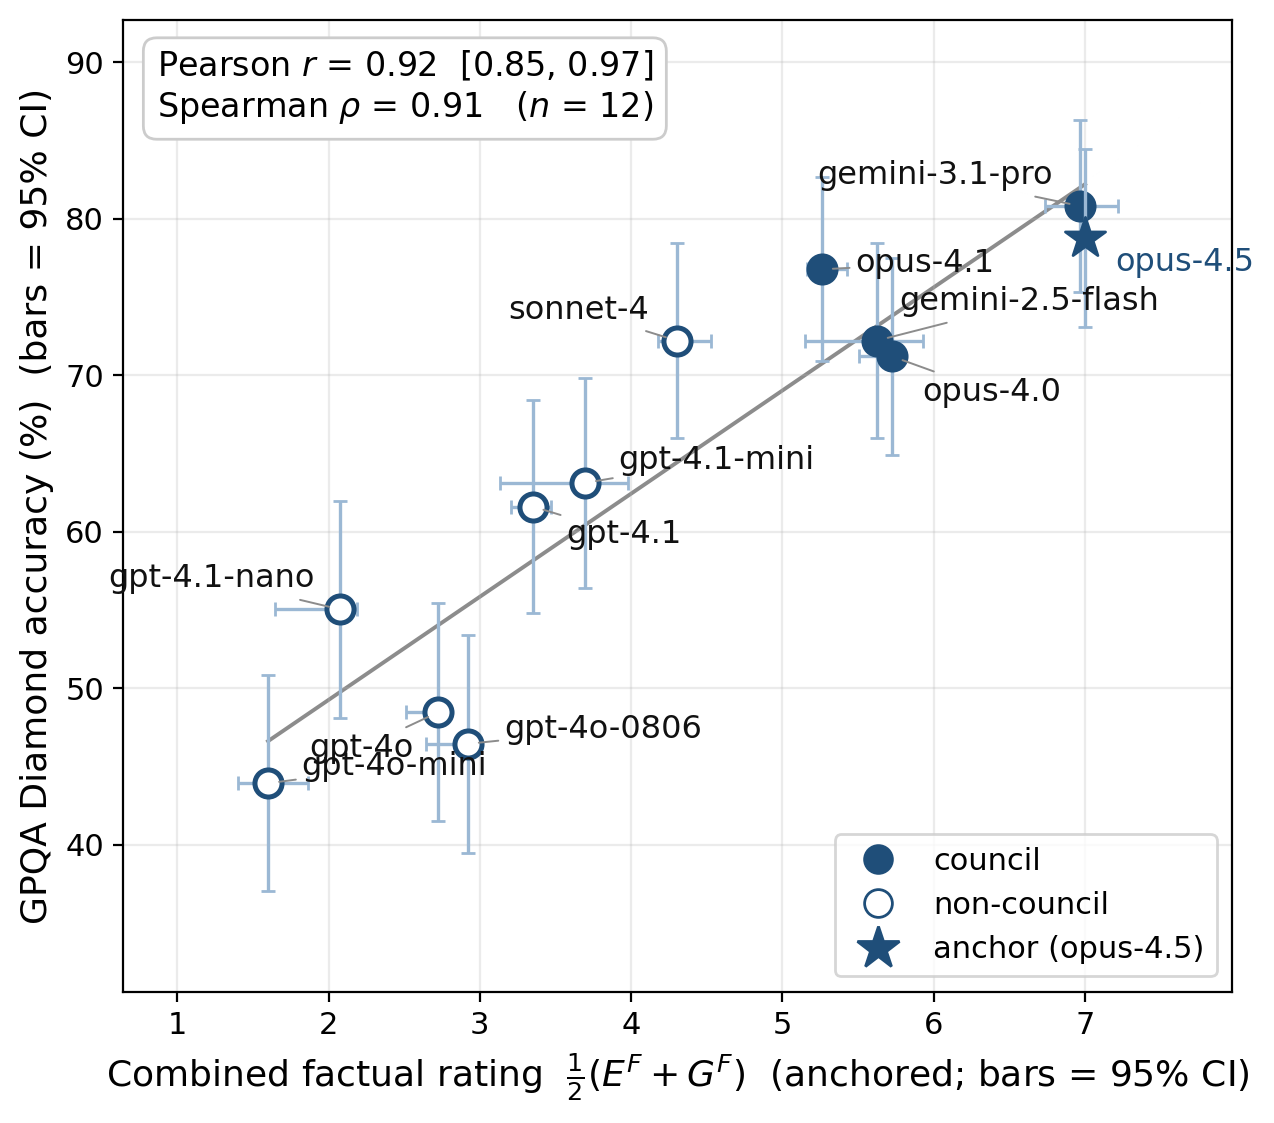
\includegraphics[width=0.85\textwidth]{figures/average_validation.png}
\caption{Combined factual rating \(\tfrac{1}{2}(E^{F}+G^{F})\) (key-free, anchored 1--10) against self-administered GPQA Diamond accuracy, across the twelve models. Plotted from the Criterion A table of §4.3 (Table~\ref{tab:criterion-a}) and the self-administered GPQA accuracies. Pearson \(r = 0.92\) (95\% CI \([0.85, 0.97]\)), Spearman \(\rho = 0.91\), \(n = 12\). Filled markers are council seats, open markers non-council; horizontal bars are the combined 95\% CI (the mean of the \(E^{F}\) and \(G^{F}\) intervals), vertical bars the GPQA binomial 95\% CI. The blue star is the anchor (opus-4.5): its combined rating is 7 by calibration (\(E^{F}=7\) the top SVD loading, \(G^{F}=7\) the reference), with GPQA measured independently --- so it is a legitimate point and is included; its \(x\) is exact, hence no horizontal bar. Excluding it leaves Pearson at 0.92.}\label{fig:gpqa-scatter}
\end{figure}

\begin{table}[H]
\centering
\caption{Council factual ratings vs self-administered GPQA Diamond accuracy.}\label{tab:gpqa-correlations}
\par\nobreak\smallskip
{\tablefont\footnotesize\setlength{\tabcolsep}{0pt}\renewcommand{\arraystretch}{1.5}
\begin{tabular}{>{\raggedright\arraybackslash}m{4.6cm} >{\centering\arraybackslash}m{0.9cm} >{\centering\arraybackslash}m{1.6cm} >{\centering\arraybackslash}m{1.6cm}}
\toprule
\multicolumn{1}{l}{\textbf{Correlation}} & \multicolumn{1}{c}{\textbf{$n$}} & \multicolumn{1}{c}{\textbf{Pearson}} & \multicolumn{1}{c}{\textbf{Spearman}}\\
\midrule
$\tfrac{1}{2}(E^{F}+G^{F})$ vs GPQA & 12 & \cellcolor[HTML]{1A2B7D}\textcolor[HTML]{FFFFFF}{0.92} & \cellcolor[HTML]{1E2F87}\textcolor[HTML]{FFFFFF}{0.91}\\
$E^{F}$ vs GPQA & 12 & \cellcolor[HTML]{243E99}\textcolor[HTML]{FFFFFF}{0.84} & \cellcolor[HTML]{1E2F87}\textcolor[HTML]{FFFFFF}{0.89}\\
$G^{F}$ vs GPQA & 11 & \cellcolor[HTML]{23469C}\textcolor[HTML]{FFFFFF}{0.82} & \cellcolor[HTML]{2253A3}\textcolor[HTML]{FFFFFF}{0.82}\\
$E^{F}$ vs $G^{F}$ & 11 & \cellcolor[HTML]{269AC1}\textcolor[HTML]{FFFFFF}{0.59} & \cellcolor[HTML]{225DA7}\textcolor[HTML]{FFFFFF}{0.75}\\
\bottomrule
\end{tabular}
}
\end{table}

Three conclusions follow.

\textbf{The metanym factual rating is relevant.} It tracks GPQA closely (combined \(r = 0.92\)), so it measures real factual capability. The two are independent instruments; their close agreement is mutual corroboration, not validation by an oracle --- GPQA is no golden key, is not assumed more accurate than the metanym rating, and the concordance simply makes it improbable that either sits far from the truth (§5.6).

\textbf{The metanym benchmark measures both the ability to say something true and the ability to find errors.} Making a true claim and spotting a false one are different skills (West et al.~2024; Oh et al.~2024; Li et al.~2024). Our benchmark confirms this. The GPQA-benchmark correlates excellently with the average value of both abilities (\(r = 0.9\)). It correlates somewhat weaker with each one of them (\(r = 0.8\)). The weakest correlation is between the two (\(r = 0.6\)). What the metanym benchmark adds to the existing methods for detecting the difference between them is getting the generating and evaluating abilities for all models in a single shot. Letting the LLMs evaluate and rate each other's statements turns it into an eigenvalue equation that we solve with SVD, finding the point where the weights of the evaluators are consistent with the evaluations.

We note that the Gemini models rank higher as judges than as makers, the Claude models the reverse (sharp for gemini-3.1-pro and sonnet-4; the rest within the error bars). This breaks the assumption behind key-free peer rankers like PiCO (Ning et al.~2025) and UPME (Zhang et al.~2025), which treat a strong maker as a strong judge. The total rating keeps the two apart (§4.6).

\hypertarget{robustness-to-regeneration}{%
\subsubsection{4.8 Robustness to regeneration}\label{robustness-to-regeneration}}

The leaderboard of §4.6 rests on one portfolio per model. To check that the result is not an artefact of that single draw, we re-ran the full pipeline three times --- the bootstrap run and two further runs produced the same day, two hours apart --- each regenerating all twelve portfolios at T=0 and re-scoring them against the frozen anchor. The regeneration is substantive: at T=0 the gateway is not deterministic, eleven of twelve portfolios differ between runs, and a total can move by as much as 0.8 between the two same-day runs (gemini-3.1-pro, 7.17→7.99).

The benchmark's categorical and ordinal outputs are robust to this. The council is \textbf{identical} across all three runs (the same five seats), and the total-rating ranking is preserved (Table~\ref{tab:reruns}) --- pairwise Pearson 0.94--0.97 and Spearman 0.93--0.95 (0.94 / 0.94 between the two same-day runs alone).

\begin{longtable}[]{@{}lrrrr@{}}
\caption{Total rating \(T\) across three full re-runs (run 1 = bootstrap; runs 2--3 the same day, two hours apart). \(\star\) marks a council seat --- the five seats are identical across all three runs. SD is the per-model run-to-run standard deviation (mean 0.38, max 0.66, both Gemini seats highest).}\label{tab:reruns}\tabularnewline
\toprule
Model & \(T_1\) & \(T_2\) & \(T_3\) & SD\tabularnewline
\midrule
\endfirsthead
\toprule
Model & \(T_1\) & \(T_2\) & \(T_3\) & SD\tabularnewline
\midrule
\endhead
\(\star\) claude-opus-4.5 & 7.00 & 7.00 & 7.00 & 0.00\tabularnewline
\midrule
\(\star\) gemini-3.1-pro & 6.69 & 7.17 & 7.99 & 0.66\tabularnewline
\midrule
\(\star\) claude-opus-4.0 & 6.21 & 5.73 & 6.56 & 0.42\tabularnewline
\midrule
\(\star\) claude-opus-4.1 & 6.05 & 6.79 & 6.57 & 0.38\tabularnewline
\midrule
\(\star\) gemini-2.5-flash & 5.76 & 5.45 & 4.67 & 0.56\tabularnewline
\midrule
claude-sonnet-4 & 5.30 & 5.47 & 6.11 & 0.43\tabularnewline
\midrule
gpt-4.1-mini & 4.74 & 5.52 & 4.91 & 0.41\tabularnewline
\midrule
gpt-4.1-2025-04-14 & 4.44 & 4.66 & 5.26 & 0.42\tabularnewline
\midrule
gpt-4o-2024-08-06 & 3.48 & 3.02 & 3.70 & 0.35\tabularnewline
\midrule
gpt-4.1-nano & 3.22 & 3.33 & 2.45 & 0.48\tabularnewline
\midrule
gpt-4o & 2.93 & 2.90 & 3.48 & 0.33\tabularnewline
\midrule
gpt-4o-mini & 2.24 & 2.33 & 2.15 & 0.09\tabularnewline

\bottomrule
\end{longtable}

The cardinal totals carry wider uncertainty than the within-run bootstrap of §4.6 conveys: the per-model run-to-run SD of \(T\) is 0.38 on average (max 0.66), and several totals move beyond their within-run interval between runs. The bootstrap measures dispersion across the 275 contexts of \emph{one} generation, not the generation being itself a random draw; the honest interval on a total is therefore the wider resample band, and the benchmark's reliable products are council membership and rank order rather than the precise total.

External validity holds on both counts: the key-free factual rating tracks GPQA Diamond at Pearson 0.86--0.92 and Spearman 0.90--0.92 across the three runs --- all inside the reported interval \([0.85, 0.97]\) (§4.7). Unlike the cardinal totals, the GPQA correlation's published CI already covers its run-to-run variation.

\hypertarget{discussion}{%
\subsection{5. Discussion}\label{discussion}}

\hypertarget{a-benchmark-by-llms-for-llms}{%
\subsubsection{5.1 A benchmark by LLMs, for LLMs}\label{a-benchmark-by-llms-for-llms}}

The aim is a benchmark that needs nothing outside itself: models invent the test, sit it, grade it, and certify which of them are fit to grade --- no human raters, no gold key, and no oracle model whose word is taken as truth. LLM-as-judge already removes the human rater (Zheng et al.~2023; Liu et al.~2023; Verga et al.~2024; Bai et al.~2023) but still requires an external ground truth --- a gold key or reference answer --- to score against. The metanym benchmark removes that dependency too --- but key-free grading is not the novelty; the unsupervised peer-evaluation line (PiCO, UPME) already gets there (§5.5). What is new is self-containment: the panel authors the very items it judges, so the test refers only to itself, and one decomposition scores the models as both makers and judges (§5.5). The benchmark is in this sense fully self-contained.

The metanym benchmark correlates excellently with GPQA. The latter is no golden key, and does not come across as more accurate than the metanym benchmark. Both occasionally reverse the expected internal ranking order within families of LLMs, such as placing a newer version of a model below its predecessor. While most of these instances are within the error margins, two examples fall outside: GPQA ranks Claude-sonnet-4 \emph{above} Claude-Opus-4.0 while the metanym benchmark places opus comfortably above sonnet. Both benchmarks rank gpt-4.1-mini \emph{above} gpt-4.1.

Both benchmarks will increase resolution following the same principle, but only the metanym benchmark does it easily. For GPQA it means engaging domain experts to increase the number of Google-proof multiple-choice questions, re-validating the test and publishing a new version of the benchmark. For the metanym benchmark the resolution is increased by twisting a knob, raising the number of archetypal contexts in a submission (here set to five).

\hypertarget{two-self-consistencies-two-yardsticks}{%
\subsubsection{5.2 Two self-consistencies, two yardsticks}\label{two-self-consistencies-two-yardsticks}}

With no outside ruler to appeal to, the yardsticks must come from the system's own structure. They come in two forms --- one for objective criteria, one for subjective --- which is why the method uses two estimators, not one.

The factual estimator rests on one assumption: \emph{the only thing competent evaluators share is the truth}. When that holds, agreement concentrates on truth, and the leading eigenvector of the leniency-removed agreement matrix is the competence axis. The warrant holds for facts and fails for taste: on \textbf{beauty}, the dominant axis of agreement is no longer truth but shared convention --- house style, training data --- so weighting by it would \emph{launder conformity into competence}, rewarding the evaluator nearest the mean and penalising a legitimate minority view. The subjective criteria therefore use the other route, \textbf{anchor-shift consistency}: the calibration reference is swept, and a competent evaluator preserves its ranking as it moves, without needing to agree with any peer. The test has teeth precisely because the shift is non-semantic: if merely moving the calibration point reorders how a model rates the same items, it has no firm grip on what it is judging --- and a stable standard is the whole of what competence means on a criterion with no external truth. One route is a consensus eigenmode across evaluators, the other an invariance within each; both are self-consistency conditions set by the system's own structure rather than an absolute scale.

\hypertarget{a-sustainable-yardstick}{%
\subsubsection{5.3 A sustainable yardstick}\label{a-sustainable-yardstick}}

The benchmark yardstick is calibrated on the \emph{anchor submission} (here the submission by Claude-opus-4.5) and the official benchmark ratings are set by the council. With model temperature T=0, no thinking or tools, the council members' evaluations are deterministic and reproducible, meaning anyone with access to the models can confirm a benchmark rating.

What varies over time is the anchor submission and the members of the council. By accounting for the changes of both over time, older benchmark ratings can be converted to approximate a rating by a newer standard; to keep that chain from drifting, each conversion is recalibrated against the archived original anchors rather than only the latest inherited factor, so error does not accumulate. An updated official rating is done by the sitting council.

This also allows changing the council size. In this paper we seat five, mainly because only five clear the factual-competence bar --- the natural sixth, Sonnet-4, is a good generator yet its factual competence as an evaluator sits in the inert band (\textasciitilde1.6), so it is not trusted to judge. The council is initially supply-limited by competence but can grow as the field improves.

\hypertarget{generating-vs-evaluating-the-truth}{%
\subsubsection{5.4 Generating vs evaluating the truth}\label{generating-vs-evaluating-the-truth}}

Making and judging factual truth are different abilities, and the council measures both and keeps them apart (§4.3). A benchmark that scored only generation would miss judging competence --- the very thing the council gate selects on --- so it is the separation, not just the rating, that lets the panel pick judges rather than only rank makers.

\hypertarget{where-this-sits-intelligence-tests-and-peer-evaluation-methods}{%
\subsubsection{5.5 Where this sits: intelligence tests and peer-evaluation methods}\label{where-this-sits-intelligence-tests-and-peer-evaluation-methods}}

Two axes locate the metanym game --- \emph{what intelligence it tests} and \emph{how self-contained the apparatus is} --- and prior work tends to be strong on one while weak on the other: the analogy benchmarks hit the target but need an external key, and the unsupervised peer-evaluation methods are key-free but aim at general capability rather than a defined, falsifiable operation.

\textbf{As an intelligence test}, the game probes the same abstraction-and-analogy cluster a long tradition places at the centre of thinking (Gentner 1983; Hofstadter \& Sander 2013; Penn, Holyoak \& Povinelli 2008; Chollet 2019; Mitchell 2021), and it probes it harder. Where the classical instruments --- BIG-Bench analogy items, Webb, Holyoak \& Lu (2023), Lewis \& Mitchell (2024), and the visual ARC-AGI (Chollet 2019) --- test one mapping over one domain pair per item, in a \emph{recognition} frame, the metanym game asks for many coupled slots across several unrelated domains, built from scratch and falsifiable per sentence (§2.c). This makes it a new \emph{kind} of analogy test, not merely a harder instance: recognition instruments \emph{select} a mapping, and the analogy-generation literature \emph{produces} one but grades it holistically, whereas the metanym game is the first to make analogical \emph{production} falsifiable sentence by sentence. That property does double duty --- it is also what lets the test be scored without a key, which is the second difference: \textbf{none of the prior instruments is self-contained.} Every one scores against an external truth --- gold labels (BIG-Bench, ARC-AGI) or paid human raters (Webb-Holyoak-Lu) --- so none can run, let alone improve, without an external oracle. They measure a similar intelligence; they cannot certify it themselves.

\textbf{As a self-contained method}, the council sits in the \emph{unsupervised peer-evaluation} line --- and that line already removes the gold key, so removing it is not what we add. Single-judge protocols (MT-Bench; G-Eval, Liu et al.~2023) score against a reference; PoLL (Verga et al.~2024) adds a panel but trusts it as given; LLM-as-Examiner (Bai et al.~2023) lets the examiner write the questions; and most directly, PiCO (Ning et al.~2025) lets unlabelled models answer and grade one another and recovers an ability ordering from peer agreement alone, with no human labels and no key (UPME, Zhang et al.~2025, extends the same peer-review idea to multimodal vision-language evaluation). What we add is two things those methods lack. \emph{First}, they apply one consensus mechanism to every dimension, which on subjective criteria rewards the model nearest the mean --- the mainstreaming §5.2 refuses; we weight by agreement only where agreement is licensed to mean truth (factual), and use anchor-shift consistency elsewhere. \emph{Second}, they grade pre-existing unlabelled questions, where ours is a purpose-built, per-sentence-falsifiable production task. The council also certifies and re-contests its own judges (§3.5) rather than trusting the panel as given. The estimator differs too, and this is the sharper break: PiCO fits one ability parameter per model by consistency optimization --- it is not a spectral method. Spectral aggregation has its own label-free lineage --- Parisi et al.~(2014) read predictor competence off the leading eigenvector of their covariance, Dawid \& Skene (1979) the EM antecedent --- but that lineage is \emph{one-sided}: its predictors classify a fixed \emph{external} dataset, so the decomposition scores the raters (rows) and recovers the hidden labels (columns), with no maker to score because no agent produced the items. Our columns are authored by the same agents on the rows, so the matrix is \emph{two-sided}: one graded SVD (§4.3) reads competence off both axes --- judges from the left singular vector, makers from the right --- and the making--judging gap (§4.7) is definable only because the test is self-produced. That two-sidedness is where self-containment lives: nothing in the matrix comes from outside it. (Parisi is binary besides; we use the graded \(1\)--\(10\) ratings, not binarised verdicts.) To our knowledge the spectral route has not been applied to LLM peer evaluation, where the unsupervised line uses EM- and optimization-based aggregation instead.

Two of our components have their own recent literature, and we use them rather than claim them. \emph{Anchor-shift consistency} applies the standard judge-reliability principle --- a competent judge is invariant under non-semantic perturbation --- to a sweep of the calibration value. Invariance-under-perturbation has been used to gate judges on criteria that have a latent truth (safety: Policy Invariance, Weng et al.~2026) or as a general diagnostic (JudgeSense, Bellibatlu et al.~2026; PiCO, Ning et al.~2025). We use calibration-invariance to certify evaluator competence on subjective, ground-truth-free criteria --- beauty, structural diversity --- where neither a gold key nor consensus-as-truth is available, and a stable standard is the only competence there is to measure; we read it as a key-free, per-criterion gate orthogonal to the spectral estimator. To our knowledge that use is new. And anchor \emph{choice} is studied directly by Don-Yehiya et al.~(2026), who find that extreme anchors discriminate poorly and that the anchor should track the capability of the cluster under comparison and rise as the field improves --- which is our recalibration rule (§5.3). Their pairwise caution about a top anchor does not bite our setup: the bootstrap winner is pinned at 7 with headroom above it and scored cardinally, and anchoring nearly \emph{doubled} the resolution F-statistic (§4.2) rather than compressing it.

The two axes meet in one sentence. Prior work offers either a test of this intelligence that needs an external key, or a key-free evaluation method aimed at general capability rather than a defined cognitive operation. The metanym game is the only one that is both --- a structural-intelligence test that certifies its own ground.

\hypertarget{self-containment-as-a-bootstrap}{%
\subsubsection{5.6 Self-containment as a bootstrap}\label{self-containment-as-a-bootstrap}}

Self-consistency builds the yardsticks; self-containment lets the apparatus improve itself. With no external dependency, the council can govern not just the scores but the \emph{rules} --- rubric, anchor, protocol, estimators. The gain is exponential rather than linear for a first-order reason: a more capable panel improves the rules more, so the increment to competence scales with the competence already present (\(\dot C \propto C\)). This is Engelbart's bootstrapping --- recursion applied to the means of improvement, not just the output --- and as models improve, the most capable panel is the one best placed to decide what to improve next.

Four of the five autonomy properties are demonstrated: the models generate the items, truth is recovered key-free, the loop runs deterministically with no human intervention, and the panel certifies its own judges. The fifth, self-improvement, is specified but not yet exercised --- the canonical run is council version 0 and includes no promotion round (§3.5). Closing that gap --- running a contest end to end, testing an anchor recalibration, and eventually allowing the council to revise a rule while the factual axis remains answerable to independent re-validation --- is what would turn a self-contained loop into a self-sustaining one.

\hypertarget{scope}{%
\subsubsection{5.7 Scope}\label{scope}}

Three caveats bound the present run. It characterises a single configuration --- one prompt template, one twelve-model roster, one anchor value --- so the bootstrap intervals measure dispersion across items, not the generation being itself a random draw --- a three-fold regeneration (§4.8) shows the council and ranking survive resampling while cardinal totals carry a wider run-to-run band --- and the anchor sweep closes the calibration axis (four values giving the same leaderboard, pairwise Spearman 0.90--0.96). Within the leading group the panel sits at its discrimination floor: the two Gemini seats are a statistical tie on the generation rating (§4.5), and fine within-group ranking is evaluator-generation-bound --- it sharpens as the seats improve and as the number of archetypal contexts is raised (§3.5). And the self-improvement loop is specified but unrun (§5.6). The deterministic, single-pass protocol (T=0, no reasoning, no tools) is a choice for reproducibility, not a sampling limit: anyone with the models reproduces the ratings exactly.

\begin{center}\rule{0.5\linewidth}{0.5pt}\end{center}

\hypertarget{summary}{%
\subsection{6. Summary}\label{summary}}

The \emph{metanym game} is a structural test of intelligence. A player discerns an \emph{archetypal context} --- an abstract system structure that recurs across unrelated domains --- writes it as a literal \emph{context template}, and instantiates the template across domain after domain by substituting \emph{metanyms}, metaphorically synonymous keywords, leaving the surrounding prose fixed; each instantiation is a \emph{parallel context}, a metaphor of the others, and because only the keywords change, the analogy is falsifiable sentence by sentence. It exercises the cluster of cognitive constructs a long tradition places at the centre of thinking (§2.c), and it is a \emph{production} task --- the player builds the structure, not merely recognises one. This makes it a new kind of analogy test: to our knowledge the first to make analogical \emph{production} falsifiable sentence by sentence (§5.5).

The \emph{council-of-peers benchmark} turns the game into a benchmark that needs nothing outside itself: twelve frontier LLMs generate portfolios and blindly cross-evaluate them, with no human raters and no gold key. Its yardsticks come from the panel's own structure rather than an external standard, through two self-consistency conditions chosen by whether the criterion is objective. For \emph{facts}, truth is recovered as the dominant axis of inter-evaluator agreement: a single SVD of the rating matrix yields both evaluator competence and item-falseness at once. For the \emph{subjective} criteria, where weighting by agreement would only launder consensus into competence, reliability is instead read from anchor-shift consistency --- an evaluator's invariance as the calibration value is swept. The panel certifies its own reliable subset, the council, on these two axes, and the seats are contestable: a stronger model can earn one on the benchmark's own rating. One external step remains, by design: a one-time validation that the key-free factual rating agrees with an independent benchmark (GPQA Diamond, \(r = 0.92\)). It is a check on the method, not a standing key in the loop.

What sets the council apart from other key-free peer-evaluation methods (§5.5) is \emph{how} the panel grades itself: it recovers competence spectrally, from a single graded SVD, where those methods optimize a per-model consistency objective; it weights by agreement only where agreement is licensed to mean truth and reads reliability from anchor-shift consistency elsewhere; it validates the factual axis once against independent tests, so its self-consistency is checked against the world and not only against itself; and it scores a defined, per-sentence-falsifiable operation rather than general capability. The empirical payoff is a dissociation the benchmark is built to see because it rates making and judging separately: \textbf{judgment is the bottleneck.} Most models cannot reliably tell a true cross-domain claim from a false one even when they generate competent structure --- the strongest generators are middling judges, the sharpest judge a mid-pack generator --- so a benchmark that conflated the two would obscure this result. (The leaderboard's one clear division tracks provider lineage rather than parameter count, but finer ordering sits below resolution and this is the least load-bearing part of the result.)

To our knowledge this is the first structural-intelligence test that certifies its own ground --- key-free, self-contained, and externally corroborated rather than externally judged --- and the first to read maker and judge competence from a single spectral decomposition of a self-produced test.

The run characterises one operating point --- Temperature 0, no reasoning, no tools --- and the self-improvement mechanism is specified but not yet exercised, so the loop is self-contained but not yet self-sustaining. The natural next steps are an open-weight panel, to separate provider-family from parameter-scale effects; a promotion round, to make the contestable council real; and a companion mechanistic study testing whether each archetypal context occupies a low-dimensional subspace of model hidden states --- which, if it holds, would give the subjective criteria the objective ground that today only factual has.

\begin{center}\rule{0.5\linewidth}{0.5pt}\end{center}

\subsection{Data and code availability}\label{data-and-code-availability}

Everything needed to check this paper is in one repository, \href{https://github.com/dnordfors/metanym-game-paper}{\texttt{github.com/dnordfors/metanym-game-paper}}: the manuscript, the arXiv submission source, the pinned evaluation runs, and the twelve analysis scripts that regenerate every number, table and figure. Running \texttt{bash\ reproduce.sh} is deterministic re-analysis of fixed model outputs --- it makes no API calls, needs no credentials, and completes in under a minute, with each step labelled by the paper exhibit it produces. Because the benchmark uses no answer key, no gold standard and no oracle model, nothing external is required to verify the ratings.

Producing a \emph{new} run --- re-querying the models for a fresh \(N\) --- is deliberately not part of that package: it costs API budget and is non-deterministic by construction. The published results derive from the runs pinned under \texttt{reproduce/data/}, and §4.8 reports what moves across three independent regenerations.

\hypertarget{references}{%
\subsection{References}\label{references}}

\hypertarget{cognitive-science-philosophy-of-science-systems-theory}{%
\subsubsection{Cognitive science, philosophy of science, systems theory}\label{cognitive-science-philosophy-of-science-systems-theory}}

\begin{enumerate}
\def\labelenumi{\arabic{enumi}.}
\tightlist
\item
  Hesse, M. (1963). \emph{Models and Analogies in Science.} London: Sheed \& Ward.
\item
  Minsky, M. (1975). A framework for representing knowledge. In P. H. Winston (Ed.), \emph{The Psychology of Computer Vision} (pp.~211--277). McGraw-Hill.
\item
  Fillmore, C. J. (1982). Frame semantics. In Linguistic Society of Korea (Ed.), \emph{Linguistics in the Morning Calm} (pp.~111--137). Hanshin.
\item
  Boyd, R. (1979). Metaphor and theory change: What is ``metaphor'' a metaphor for? In A. Ortony (Ed.), \emph{Metaphor and Thought} (pp.~356--408). Cambridge University Press.
\item
  Gentner, D. (1983). Structure-mapping: A theoretical framework for analogy. \emph{Cognitive Science, 7}(2), 155--170.
\item
  Gick, M. L., \& Holyoak, K. J. (1983). Schema induction and analogical transfer. \emph{Cognitive Psychology, 15}(1), 1--38.
\item
  Gentner, D. (1989). The mechanisms of analogical learning. In S. Vosniadou \& A. Ortony (Eds.), \emph{Similarity and Analogical Reasoning.} Cambridge University Press.
\item
  Falkenhainer, B., Forbus, K. D., \& Gentner, D. (1989). The structure-mapping engine: Algorithm and examples. \emph{Artificial Intelligence, 41}(1), 1--63.
\item
  Lakoff, G., \& Johnson, M. (1980). \emph{Metaphors We Live By.} University of Chicago Press.
\item
  Holyoak, K. J., \& Thagard, P. (1995). \emph{Mental Leaps: Analogy in Creative Thought.} MIT Press.
\item
  Goldberg, A. E. (1995). \emph{Constructions: A Construction Grammar Approach to Argument Structure.} University of Chicago Press.
\item
  Penn, D. C., Holyoak, K. J., \& Povinelli, D. J. (2008). Darwin's mistake: Explaining the discontinuity between human and nonhuman minds. \emph{Behavioral and Brain Sciences, 31}(2), 109--130.
\item
  Hofstadter, D., \& Sander, E. (2013). \emph{Surfaces and Essences.} Basic Books.
\item
  von Bertalanffy, L. (1968). \emph{General System Theory.} George Braziller.
\item
  Salthe, S. N. (1985). \emph{Evolving Hierarchical Systems: Their Structure and Representation.} Columbia University Press.
\end{enumerate}

\hypertarget{archetypes-and-pattern-instantiation}{%
\subsubsection{Archetypes and pattern-instantiation}\label{archetypes-and-pattern-instantiation}}

\begin{enumerate}
\def\labelenumi{\arabic{enumi}.}
\setcounter{enumi}{15}
\tightlist
\item
  Pauli, W. (1955). The influence of archetypal ideas on the scientific theories of Kepler (P. Silz, Trans.). In C. G. Jung \& W. Pauli, \emph{The Interpretation of Nature and the Psyche} (pp.~147--240). Pantheon Books. (Original work published 1952) \emph{(Cited for the Jung--Pauli proposal that archetypes act as ordering principles across psyche and physical world; we adopt the structural framing, not the wider metaphysics.)}
\end{enumerate}

\hypertarget{psychometric-intelligence-taxonomies}{%
\subsubsection{Psychometric intelligence taxonomies}\label{psychometric-intelligence-taxonomies}}

\begin{enumerate}
\def\labelenumi{\arabic{enumi}.}
\setcounter{enumi}{16}
\tightlist
\item
  Cattell, R. B. (1963). Theory of fluid and crystallized intelligence: A critical experiment. \emph{Journal of Educational Psychology, 54}(1), 1--22.
\item
  Horn, J. L., \& Cattell, R. B. (1966). Refinement and test of the theory of fluid and crystallized general intelligences. \emph{Journal of Educational Psychology, 57}(5), 253--270.
\item
  Guilford, J. P. (1967). \emph{The Nature of Human Intelligence.} McGraw-Hill.
\item
  Carroll, J. B. (1993). \emph{Human Cognitive Abilities: A Survey of Factor-Analytic Studies.} Cambridge University Press.
\item
  McGrew, K. S. (2009). CHC theory and the human cognitive abilities project. \emph{Intelligence, 37}(1), 1--10.
\end{enumerate}

\hypertarget{llm-as-judge-methodology}{%
\subsubsection{LLM-as-judge methodology}\label{llm-as-judge-methodology}}

\begin{enumerate}
\def\labelenumi{\arabic{enumi}.}
\setcounter{enumi}{21}
\tightlist
\item
  Zheng, L., et al.~(2023). Judging LLM-as-a-Judge with MT-Bench and Chatbot Arena. \emph{Advances in Neural Information Processing Systems (NeurIPS), 36.} arXiv:2306.05685.
\item
  Liu, Y., et al.~(2023). G-Eval: NLG evaluation using GPT-4 with better human alignment. \emph{Proceedings of EMNLP 2023.} arXiv:2303.16634.
\item
  Verga, P., et al.~(2024). Replacing judges with juries: Evaluating LLM generations with a panel of diverse models. arXiv:2404.18796.
\item
  Bai, Y., et al.~(2023). Benchmarking foundation models with Language-Model-as-an-Examiner. \emph{NeurIPS 36.} arXiv:2306.04181.
\item
  Ning, K.-P., Yang, S., Liu, Y.-Y., Yao, J.-Y., Liu, Z.-H., Wang, Y., Pang, M., \& Yuan, L. (2025). PiCO: Peer review in LLMs based on consistency optimization. \emph{Proceedings of ICLR 2025.} arXiv:2402.01830.
\item
  Zhang, Q., Ning, M., Liu, Z., Huang, Y., Yang, S., Wang, Y., Ye, J., Chen, X., Song, Y., \& Yuan, L. (2025). UPME: An unsupervised peer review framework for multimodal large language model evaluation. \emph{Proceedings of CVPR 2025.} arXiv:2503.14941.
\item
  Don-Yehiya, S., Yehudai, A., Choshen, L., \& Abend, O. (2026). Mediocrity is the key for LLM as a judge anchor selection. arXiv:2603.16848.
\item
  Weng, S., Feng, Y., \& Xie, X. (2026). Beyond accuracy: Policy invariance as a reliability test for LLM safety judges. arXiv:2605.06161.
\item
  Bellibatlu, R. R., Raff, E., \& Zhang, W. (2026). JudgeSense: A benchmark for prompt sensitivity in LLM-as-a-judge systems. arXiv:2604.23478.
\end{enumerate}

\hypertarget{analogical-reasoning-in-llms}{%
\subsubsection{Analogical reasoning in LLMs}\label{analogical-reasoning-in-llms}}

\begin{enumerate}
\def\labelenumi{\arabic{enumi}.}
\setcounter{enumi}{30}
\tightlist
\item
  Webb, T., Holyoak, K. J., \& Lu, H. (2023). Emergent analogical reasoning in large language models. \emph{Nature Human Behaviour, 7}(9), 1526--1541.
\item
  Lewis, M., \& Mitchell, M. (2024). Using counterfactual tasks to evaluate the generality of analogical reasoning in large language models. arXiv:2402.08955.
\end{enumerate}

\hypertarget{related-benchmarks}{%
\subsubsection{Related benchmarks}\label{related-benchmarks}}

\begin{enumerate}
\def\labelenumi{\arabic{enumi}.}
\setcounter{enumi}{32}
\tightlist
\item
  Chollet, F. (2019). On the measure of intelligence. arXiv:1911.01547.
\item
  Mitchell, M. (2021). Abstraction and analogy-making in artificial intelligence. \emph{Annals of the New York Academy of Sciences, 1505}(1), 79--101.
\item
  Lake, B. M., Ullman, T. D., Tenenbaum, J. B., \& Gershman, S. J. (2017). Building machines that learn and think like people. \emph{Behavioral and Brain Sciences, 40}, e253.
\item
  Srivastava, A., et al.~(2022). Beyond the imitation game: Quantifying and extrapolating the capabilities of language models. arXiv:2206.04615.
\item
  Cobbe, K., et al.~(2021). Training verifiers to solve math word problems. arXiv:2110.14168.
\item
  Rein, D., Hou, B. L., Stickland, A. C., Petty, J., Pang, R. Y., Dirani, J., Michael, J., \& Bowman, S. R. (2023). GPQA: A graduate-level Google-proof Q\&A benchmark. arXiv:2311.12022.
\end{enumerate}

\hypertarget{statistical-methods}{%
\subsubsection{Statistical methods}\label{statistical-methods}}

\begin{enumerate}
\def\labelenumi{\arabic{enumi}.}
\setcounter{enumi}{38}
\tightlist
\item
  Efron, B., \& Tibshirani, R. J. (1993). \emph{An Introduction to the Bootstrap.} Chapman \& Hall.
\item
  Parisi, F., Strino, F., Nadler, B., \& Kluger, Y. (2014). Ranking and combining multiple predictors without labeled data. \emph{Proceedings of the National Academy of Sciences, 111}(4), 1253-1258.
\item
  Dawid, A. P., \& Skene, A. M. (1979). Maximum likelihood estimation of observer error-rates using the EM algorithm. \emph{Journal of the Royal Statistical Society: Series C (Applied Statistics), 28}(1), 20-28.
\end{enumerate}

\hypertarget{generation-vs-evaluation}{%
\subsubsection{Generation vs evaluation}\label{generation-vs-evaluation}}

\begin{enumerate}
\def\labelenumi{\arabic{enumi}.}
\setcounter{enumi}{41}
\tightlist
\item
  West, P., Lu, X., Dziri, N., Brahman, F., Li, L., Hwang, J. D., Jiang, L., Fisher, J., Ravichander, A., Chandu, K., Newman, B., Koh, P. W., Ettinger, A., \& Choi, Y. (2024). The Generative AI Paradox: ``What it can create, it may not understand.'' \emph{Proceedings of ICLR 2024.} arXiv:2311.00059.
\item
  Oh, J., Kim, E., Cha, I., \& Oh, A. (2024). The Generative AI Paradox on evaluation: What it can solve, it may not evaluate. \emph{EACL 2024 Student Research Workshop.} arXiv:2402.06204.
\item
  Li, X. L., Shrivastava, V., Li, S., Hashimoto, T., \& Liang, P. (2024). Benchmarking and improving generator-validator consistency. \emph{Proceedings of ICLR 2024.} arXiv:2310.01846.
\end{enumerate}

\begin{center}\rule{0.5\linewidth}{0.5pt}\end{center}

\hypertarget{appendices}{%
\subsection{Appendices}\label{appendices}}

% --- contents of the appendices ----------------------------------------------------
% Hand-built rather than etoc/titletoc/minitoc: this preamble is hand-tuned pandoc
% output and the tarball has to build on arXiv's TeX, so no package is added for a few
% lines of navigation. Both halves of each line are keyed to pandoc's own section
% labels -- \pageref for the number, \hyperref for the title -- so the two always
% agree and nothing here can go stale. \hyperref rather than \hyperlink: pandoc's
% \hypertarget sits one line above the heading, so where a page breaks between the two
% (A.3) a \hyperlink lands at the foot of the preceding page while \pageref names the
% next one. Styled after the table-caption blocks, not as a generated table of
% contents. Second-level entries are given for Appendix A alone: its A.1--A.6 are
% independent reference definitions spread over ten pages, whereas B's title already
% names its two prompts and C and D are each one continuous worked example whose
% inner headings are content, not navigation.
\noindent\hspace*{2.5em}\begin{minipage}{\dimexpr\linewidth-5em\relax}
{\tablefont\fontsize{12}{14.5}\selectfont Contents of the appendices}\par\vskip5pt
{\tablefont\small\setlength{\parskip}{1.5pt}%
\hyperref[appendix-a.-rating-estimators]{Appendix A. Rating estimators}\hfill\pageref{appendix-a.-rating-estimators}\par
\hspace*{1.5em}\hyperref[a.1-generation-rating]{A.1 Generation rating}\hfill\pageref{a.1-generation-rating}\par
\hspace*{1.5em}\hyperref[a.2-evaluation-ratings]{A.2 Evaluation ratings}\hfill\pageref{a.2-evaluation-ratings}\par
\hspace*{1.5em}\hyperref[a.3-the-council]{A.3 The council}\hfill\pageref{a.3-the-council}\par
\hspace*{1.5em}\hyperref[a.4-the-total-rating]{A.4 The total rating}\hfill\pageref{a.4-the-total-rating}\par
\hspace*{1.5em}\hyperref[a.5-confidence-intervals]{A.5 Confidence intervals}\hfill\pageref{a.5-confidence-intervals}\par
\hspace*{1.5em}\hyperref[a.6-generationevaluation-alignment]{A.6 Generation--evaluation alignment}\hfill\pageref{a.6-generationevaluation-alignment}\par
\hyperref[appendix-b.-generation-and-evaluation-prompts]{Appendix B. Generation and evaluation prompts}\hfill\pageref{appendix-b.-generation-and-evaluation-prompts}\par
\hyperref[appendix-c.-anchor-reference-submission]{Appendix C. Anchor (reference) submission}\hfill\pageref{appendix-c.-anchor-reference-submission}\par
\hyperref[appendix-d.-council-evaluation-of-a-target-submission]{Appendix D. Council evaluation of a target submission}\hfill\pageref{appendix-d.-council-evaluation-of-a-target-submission}\par
}\vskip4pt\rule{\linewidth}{0.4pt}
\end{minipage}\par\vspace{\medskipamount}

\hypertarget{appendix-a.-rating-estimators}{%
\subsubsection{Appendix A. Rating estimators}\label{appendix-a.-rating-estimators}}

The exact estimators for every benchmark rating, all computed from one anchored, anchor-swept evaluation matrix with no external key: A.1 generation (anchored leave-self-out council means, paired bootstrap); A.2 the evaluation ratings --- A.2.a factual competence and instantiation falseness (one SVD of the verdict matrix: evaluator competence on the left, instantiation falseness --- and a generation-factuality rating --- on the right) and A.2.b criterion reliability (anchor-shift consistency --- mean pairwise Pearson, per evaluator) and A.2.c anchor sensitivity (why factual reliability is attenuated while factual validity is anchor-stable); A.3 the council (the reliable-evaluator definition); A.4 the total rating (the anchor-7 total \(T = \tfrac12(G + E) = \tfrac14(G^{F} + G^{C} + E^{F} + E^{C})\), §4.6).

\hypertarget{appendix-a.-rating-estimators-1}{%
\subsubsection{Appendix A. Rating estimators}\label{appendix-a.-rating-estimators-1}}

Every rating comes from one object: the scores the panel produces when each model grades the others' portfolios, swept across the anchor. No external answer key is used. This appendix defines that object and the estimators built on it.

\textbf{Panel and tasks.} Twelve models form the panel, indexed by \(s,t\in\{1,\dots,12\}\). Each is both a \emph{submission} (its portfolio is graded) and an \emph{evaluator} (it grades the others). Every model was in fact asked to grade every portfolio including its own, and those self-evaluations are in the released run data; but \textbf{no rating below uses a model's grade of its own portfolio} --- every estimator here is \emph{leave-self-out}. The two criteria implement that exclusion differently, and the difference is deliberate: Criterion A (A.2.a) keeps the self-entry as a column of its matrix and sets it to the anchor value (A5), so the factorisation stays on one rectangular matrix; Criterion B (A.2.b) and the generation rating (A.1) drop the self-pair from the unit set outright. Below, \(s,t\) denote a model in whichever role an equation needs --- the graded submission in A.1, the grading evaluator in A.2. A portfolio holds five \emph{archetypes} --- the templates a model produced --- each realised as several \emph{parallel contexts}, the same template instantiated in different domains. A model is rated on the two tasks of the game (§2.b): to \textbf{generate} archetypal context templates \emph{and} their instantiations, and to \textbf{evaluate} others' portfolios. It earns, correspondingly,

\begin{equation} G=\text{generation rating},\qquad E=\text{evaluation rating}. \tag{A1}\end{equation}

These yield the total rating (A14), and \(E\) has two parts (A12); each is constructed below.

\textbf{Rubric and anchor.} Scoring uses six axes, each rated on a \(1\)--\(10\) scale: a \emph{factual} axis (scored once per parallel context) and five \emph{non-factual} axes --- beauty, intelligence, instantiation-distinctness and impressive-length (once per archetype) and structural-diversity among the archetypes (once per portfolio). Every score is given relative to a fixed reference portfolio, the \textbf{anchor} --- the model \(a\) whose portfolio won the un-anchored initial selection (§4.1), declared to score \(7\) on every axis. Because \(a\) is a panel member it also evaluates; the anchor is required to be a council member (A.3), so its factual competence \(f_a>0\) and criterion competence \(\bar\rho_a>0\) (A.2). The anchor value is swept, \(\theta\in\Theta=\{5,6,7,8\}\) --- each value a separate scoring pass with the reference declared at that value --- and \(\theta^{*}=7\) is the production anchor. Write \(r_{t,s,x,u}(\theta)\) for evaluator \(t\)'s score of unit \(u\) of axis \(x\) of submission \(s\) at anchor \(\theta\).

\hypertarget{a.1-generation-rating}{%
\paragraph{A.1 Generation rating}\label{a.1-generation-rating}}

Evaluator \(t\)'s overall score of submission \(s\) averages within each axis, then across axes (so axes weigh equally although a per-portfolio axis has one unit and the factual axis has many):

\begin{equation} o_{t,s}=\frac{1}{|\mathcal{X}|}\sum_{x\in\mathcal{X}}\frac{1}{|U_x|}\sum_{u\in U_x} r_{t,s,x,u}(\theta^{*}), \tag{A2}\end{equation}

where \(\mathcal{X}\) is the axis set and \(U_x\) the units of axis \(x\). Production ratings use only the production anchor \(\theta^{*}\); the sweep \(\Theta\) enters the benchmark solely through criterion competence (A.2.b). The generation rating is the leave-self-out mean over the council \(\mathcal{C}\) (A.3):

\begin{equation} G_s=\frac{1}{|\mathcal{C}\setminus\{s\}|}\sum_{t\in\mathcal{C},\,t\ne s} o_{t,s}. \tag{A3}\end{equation}

Confidence intervals: 95\% percentile bootstrap over the per-(submission, archetype) scoring units; a gap \(G_s-G_{s'}\) is \emph{resolvable} when the paired bootstrap (resampling the same units for both models) puts its 95\% interval clear of \(0\).

\hypertarget{a.2-evaluation-ratings}{%
\paragraph{A.2 Evaluation ratings}\label{a.2-evaluation-ratings}}

The evaluation rating \(E\) measures how good a judge a model is, in two independent parts: how accurately it detects factual errors (A.2.a) and how stably it ranks work as the anchor moves (A.2.b).

\hypertarget{a.2.a-factual-competence-and-instantiation-falseness-svd}{%
\subparagraph{A.2.a Factual competence and instantiation falseness (SVD)}\label{a.2.a-factual-competence-and-instantiation-falseness-svd}}

With no key, we must find both which evaluators judge factuality well and which instantiations are factually weak. One factorisation gives both.

Stack the panel's factual scores into a matrix \(F\) (evaluators \(\times\) instantiations): \(F_{sj}\) is evaluator \(s\)'s \(1\)--\(10\) factual rating of pooled parallel context \(j\), used \textbf{directly} --- with no thresholding into a true/false verdict, so the full graded judgement is kept. A model does not grade its own submission; those self-entries are set to the anchor value (a model's own work treated as reference-clean):

\begin{equation} F_{sj}=r_{s,j}\in\{1,\dots,10\}\qquad(\text{self-entries }=\theta^{*}=7). \tag{A5}\end{equation}

Centre each row (subtract the evaluator's mean over its \(N\) entries, removing its overall leniency); only the leading triple is used:

\begin{equation} \tilde F = F-\bar r\,\mathbf 1^{\top}=U\Sigma V^{\top},\qquad \sigma_1,\quad u\equiv U_{\cdot 1},\quad v\equiv V_{\cdot 1}. \tag{A6}\end{equation}

This is the rank-one model \(\tilde F_{sj}\approx \sigma_1\,u_s v_j\). The hypothesis is that competent evaluators \textbf{agree on the centred pattern} --- which instantiations are weaker, once each evaluator's own leniency is subtracted --- and the leading axis of that agreement is the competence axis. The left singular vector is factual competence,

\begin{equation} f\equiv u,\qquad \text{signed so } \textstyle\sum_s f_s>0,\qquad f^{+}_s=\max(f_s,0), \tag{A7}\end{equation}

the quantity the council gate uses (A.3) and that \(E^{F}\) rescales (A12), clamped at zero so an evaluator anti-correlated with the consensus carries no weight. Centering is essential, not cosmetic: the raw scores cluster at the anchor (most contexts are clean, near \(7\)), so on the \emph{un}-centred matrix the leading axis is simply that shared level and ranks the most lenient --- non-detecting --- evaluators highest; subtracting each row's mean removes the level so the leading axis becomes agreement-on-pattern. (Equivalently \(u\) is the leading eigenvector of the row-centred inter-evaluator Gram \(\tilde F\tilde F^{\top}\).) Competence is a continuum, not a hard cliff: an evaluator whose centred scores are flat or idiosyncratic lands near zero, and the council gate (A.3) reads the gap above that inert band.

Because every row of \(\tilde F\) sums to zero, the all-ones vector lies in its null space, so each right singular vector is orthogonal to it and itself sums to zero: \(v\) is therefore signed, and we orient it to agree with the panel (\(\operatorname{corr}(v,\ \text{column means of }\tilde F)>0\), so positive means \emph{factually stronger} --- a cleaner instantiation, scored above the evaluators' norm). The left vector \(u\) is sign-fixed by (A7) and clamped to \(f^{+}\); on soft ratings it is not guaranteed non-negative (an evaluator can be anti-correlated with the consensus), so the clamp is an explicit convention rather than an automatic property.

The right singular vector \(v\) orders the instantiations by factual standing; to read it back on the native \(1\)--\(10\) scale we reconstruct each instantiation's rating from the rank-one model and a competence-weighted baseline. The \textbf{competence-weighted consensus rating} of instantiation \(j\) is

\begin{equation} \hat r_j \;=\; C+\kappa\,v_j,\qquad C=\frac{\sum_s f^{+}_s\,\bar r_s}{\sum_s f^{+}_s},\quad \kappa=\sigma_1\,\frac{\sum_s f^{+}_s\,u_s}{\sum_s f^{+}_s}>0, \tag{A8}\end{equation}

an affine read-off of the right vector (\(C\) the competence-weighted clean level, \(\kappa\) the rank-one scale). It is exactly the rank-one approximation of the competence-weighted mean rating \(\big(\sum_s f^{+}_s F_{sj}\big)/\sum_s f^{+}_s\), the two differing only by the discarded higher-rank residual. Averaging over a generator's own instantiations \(J_g\) gives the key-free \textbf{generation-factuality} rating

\begin{equation} G^{F}_{\text{svd},g} \;=\; \frac1{|J_g|}\sum_{j\in J_g}\hat r_j. \tag{A9}\end{equation}

No \(\times7\) rescaling is needed --- the rating is already on the \(1\)--\(10\) scale: clean instantiations sit at \(v_j\approx0\), hence at \(C\approx7\), so a reference-clean portfolio scores \(\approx7\) by construction (the declared-clean reference scores \(7\) exactly, not measured). \(G^{F}_{\text{svd}}\) is a generation-side factual rating, reported beside \(G\) and \textbf{not} part of the evaluation total \(T\) (A14).

This is the exact dual of (A7): the \textbf{left} singular vector rates an evaluator's competence at \emph{spotting} a factually weak instantiation; the \textbf{right}, aggregated to generators through (A8)--(A9), rates a generator's competence at \emph{producing a sound} one --- both from the one factorisation, with no key. \(G^{F}_{\text{svd}}\) carries a 95\% bootstrap CI computed by resampling each generator's own instantiation ratings \(\hat r_j\) (the (submission, archetype) unit of A.5) with the panel consensus \((C,\kappa,v)\) held fixed --- the dominant source of a generator's uncertainty being the spread of its own instantiations.

\emph{Why it works.} Better judges converge on the same relative assessment; their shared axis is that consensus; on a vendor-diverse panel with no common bias, the consensus is the truth. The lone assumption is that the only thing the evaluators share is the truth --- a same-vendor bloc with a common bias would add a spurious shared component --- so competence is read off a vendor-diverse panel with a shared-bias check (§4.3). \(f\) carries a 95\% bootstrap CI over the \(N\) contexts; the council (A.3) admits \(s\) only when that CI sits clear of the inert band.

\hypertarget{a.2.b-criterion-competence}{%
\subparagraph{A.2.b Criterion competence}\label{a.2.b-criterion-competence}}

An evaluator's \textbf{criterion competence} is its capacity to hold a stable standard for each non-factual criterion; we measure it by \emph{anchor-shift consistency}. A reliable evaluator ranks portfolios the same way wherever the anchor sits; only the absolute numbers should move. The anchor is set to each of the four swept values \(5, 6, 7, 8\) in turn (\(7\) is the value used in production), and we ask whether the evaluator's ranking survives the shift. The Pearson correlation captures exactly this: it is unchanged by a common shift or stretch, so the harmless rise from raising the anchor costs nothing and only a genuine reordering does.

For evaluator \(s\) and axis \(x\), let \(v_{s,x}(\theta)\) be \(s\)'s axis-\(x\) scores across that axis's units at anchor \(\theta\). Eleven portfolios are graded --- the anchor's own is the fixed reference, not a graded free-generation submission --- so an evaluator that is itself one of the eleven is scored, leave-self-out, on the other \textbf{ten}: \(50=10\times5\) units for the four per-archetype non-factual axes, \(250=10\times25\) parallel contexts for factual, and \(10\) portfolios for structural-diversity. The anchor \(a\) is the exception: its portfolio is not among the eleven, so it grades all of them and its unit counts are \(55\), \(275\) and \(11\). (Throughout, the two submissions that returned a sixth archetype contribute their first five archetypes only, so every portfolio weighs \(5\) archetypes and \(25\) contexts --- this is the same balancing that gives Criterion A its \(275\) columns. These are design counts; observed coverage meets them for eight of the twelve evaluators and falls short where a grading call did not return --- by one archetype for claude-sonnet-4 and gpt-4o-mini, and by two whole portfolios for gpt-4.1-nano, which grades \(8\) rather than \(10\). A missing entry is dropped pairwise by the correlation in (A10)--(A11), so a shortfall costs units, not correctness.) The per-axis criterion competence --- its anchor-shift consistency on that axis --- is the average Pearson correlation over the anchor pairs on which it is defined,

\begin{equation} \rho_{s,x}=\frac{1}{|\mathcal P_{s,x}|}\sum_{(\theta,\theta')\in\mathcal P_{s,x}}\operatorname{corr}\!\big(v_{s,x}(\theta),v_{s,x}(\theta')\big), \tag{A10}\end{equation}

where \(\mathcal P_{s,x}\) is the subset of the \(\binom{4}{2}=6\) anchor pairs for which both score vectors are non-constant (a constant vector makes the correlation undefined, so that pair is dropped). This per-axis breakdown is the diagnostic \textbf{per-criterion competence} \(E^{C}_a=\rho_{s,x}\) (\(a\) ranging over the non-factual axes --- beauty, intelligence, instantiation-distinctness, impressive-length, structural-diversity; §4.4). The single \textbf{criterion-competence} score \(\bar\rho_s\) that gates the council is not the mean of (A10) but a single collapsed score: average the four non-factual per-archetype axes (beauty, intelligence, instantiation-distinctness, impressive-length) into one value per (submission, archetype), giving a vector \(v_{s}(\theta)\) over \(s\)'s \(50\) leave-self-out units (\(55\) for the anchor), and take

\begin{equation} \bar\rho_s=\frac{1}{|\mathcal P_{s}|}\sum_{(\theta,\theta')\in\mathcal P_{s}}\operatorname{corr}\!\big(v_{s}(\theta),v_{s}(\theta')\big), \tag{A11}\end{equation}

with \(\mathcal P_s\) the anchor pairs on which \(v_s\) is non-constant. Factual is A.2.a's job and is excluded; structural-diversity, one score per portfolio, is too coarse for a per-archetype vector and is excluded too. The council gate (A.3) uses \(\bar\rho_s\ge0.78\). These statistics use only \(s\)'s own scores, so they are independent of the rest of the panel --- which is why the leave-self-out convention here cannot cascade into A.2.a. \(\bar\rho_s\) is reported with a bootstrap CI resampled over the full \(55\)-atom (submission, archetype) grid of A.5, the same grid every CI in this paper uses; each evaluator then contributes whichever of the resampled atoms are among its own \(50\) (the anchor's \(55\)). The two numbers are distinct and both are needed: \(55\) is the shared resampling grid, \(50\) is one graded evaluator's effective sample.

\hypertarget{a.2.c-anchor-sensitivity-why-factual-consistency-is-attenuated-while-factual-competence-is-anchor-stable}{%
\subparagraph{A.2.c Anchor sensitivity: why factual consistency is attenuated while factual competence is anchor-stable}\label{a.2.c-anchor-sensitivity-why-factual-consistency-is-attenuated-while-factual-competence-is-anchor-stable}}

If anchor-shift consistency (A.2.b) is computed on the factual axis (\(E^{C}_f\), a diagnostic only --- factual is gated by \(f\), not by consistency), it comes out low --- panel mean \(0.63\), against \(0.67\)--\(0.70\) for beauty, intelligence, impressive-length and structural-diversity; yet the factual competence \(f\) (A.2.a) is essentially unchanged as the anchor is swept. Both facts follow from one first-order model of what the anchor does. Declaring the reference at value \(\theta\) reparameterises each evaluator's scale; to first order each score is

\begin{equation} r_{s,x,u}(\theta)=\alpha_{s,x}(\theta)+\beta_{s,x}(\theta)\,t_{s,x,u}+\varepsilon_{s,x,u}(\theta), \tag{A11a}\end{equation}

with \(t_{s,x,u}\) the evaluator's anchor-free latent assessment of unit \(u\) (the \emph{signal}, with axis-dependent variance \(\sigma_x^2=\operatorname{Var}_u\,t_{s,x,u}\)), \(\alpha_{s,x}(\theta)\) a leniency offset, \(\beta_{s,x}(\theta)>0\) a scale, and \(\varepsilon\) zero-mean idiosyncratic noise --- the part of the score the anchor reshuffles non-systematically --- taken independent of the signal \(t\) and across anchors, with variance \(\sigma_\varepsilon^2\) common across evaluators and anchors.

\textbf{Reliability (A.2.b) is attenuated by the axis signal variance.} Pearson is invariant to the affine \((\alpha,\beta)\), so for an anchor pair, with \(\beta_{s,x}\) steady across the pair (here \(v_{s,x}(\theta)\) is evaluator \(s\)'s axis-\(x\) score vector of A.2.b, eq A10 --- not the right singular vector \(v\) of A.2.a),

\begin{equation} \operatorname{corr}\!\big(v_{s,x}(\theta),v_{s,x}(\theta')\big)\;\approx\;\frac{\beta_{s,x}^{2}\,\sigma_x^{2}}{\beta_{s,x}^{2}\,\sigma_x^{2}+\sigma_\varepsilon^{2}}\;=\;\frac{\mathrm{SNR}_x}{1+\mathrm{SNR}_x},\qquad \mathrm{SNR}_x=\frac{\beta_{s,x}^{2}\,\sigma_x^{2}}{\sigma_\varepsilon^{2}}. \tag{A11b}\end{equation}

This is the classical test--retest attenuation: holding \(\beta\) and \(\sigma_\varepsilon^2\) fixed, \(\rho_{s,x}\) increases monotonically with the axis signal variance \(\sigma_x^{2}\) (across axes \(\beta\) and \(\sigma_\varepsilon^2\) may also differ, so no ordering among the axes follows from \(\sigma_x^{2}\) alone). The factual axis carries the smallest \(\sigma_x^{2}\). It is scored once per parallel context, and most instantiations are simply true, so factual ratings pile against the ceiling --- an observable proxy for that compressed signal variance: on the anchor-\(7\) matrix, leave-self-out over archetypes \(1\)--\(5\), the within-evaluator factual SD is \(1.04\), the lowest of the six axes (the SD also carries the noise term, but it is the ceiling pile-up that compresses \(\sigma_x^2\)), with \(72\%\) of factual ratings \(\ge 7\) against \(35\)--\(55\%\) on the other five. Smallest \(\sigma_x^{2}\Rightarrow\) smallest SNR \(\Rightarrow\) strongest attenuation \(\Rightarrow\) depressed consistency.

\textbf{What the data show, and where they do not fit.} The prediction is corroborated in part. Factual consistency --- \(0.63\) across the panel, \(0.74\) across the council --- sits below the four axes whose ratings are not compressed against the ceiling (\(0.67\)--\(0.70\) and \(0.82\)--\(0.87\) respectively), which is the footprint (A11b) predicts of a compressed signal. Factual is not, however, the lowest axis: instantiation-distinctness is, at \(0.59\) and \(0.72\), and the ceiling mechanism does not explain it --- only \(55\%\) of distinctness ratings sit at \(\ge 7\) and its within-evaluator SD (\(1.10\)) is mid-pack, so its low consistency reflects not a compressed signal but an absent shared standard: evaluators disagree with \emph{themselves} about how distinct two instantiations of one template are. (A11b) therefore licenses one claim and no more --- that a depressed factual \(\rho_{s,x}\) is the expected footprint of a compressed signal --- and no ordering over the remaining axes. Because the axes differ in \(\sigma_x^{2}\), in unit of analysis (parallel context vs archetype), and hence in SNR, their consistencies are \textbf{not commensurable}, which is why \(E^{C}\) is collapsed over the four comparable per-archetype axes and factual is gated by \(f\) instead.

\textbf{Validity (A.2.a) is protected by row-centering.} Specialising (A11a) to the factual axis (\(x\) fixed, so the units are now the instantiations \(j\), matching A.2.a's columns) and stacking into \(F(\theta)\), row-centring as in (A6) subtracts each evaluator's row mean \(\alpha_s(\theta)+\beta_s(\theta)\bar t_s+\bar\varepsilon_s\), cancelling the anchor offset \(\alpha_s(\theta)\) exactly:

\begin{equation} \tilde F_{sj}(\theta)=\beta_s(\theta)\,(t_{sj}-\bar t_s)+(\varepsilon_{sj}-\bar\varepsilon_s). \tag{A11c}\end{equation}

Under the rank-one signal model \(t_{sj}-\bar t_s\approx c_s\,w_j\) --- where \(c\) (competence pattern) and \(w\) (item truth) are the latent quantities the empirical left and right vectors \(u=f\) and \(v\) of (A6) estimate --- the leading left singular vector of \(\tilde F(\theta)\) is \(f\propto \beta(\theta)\!\circ\! c\). The offset --- the dominant effect of moving the anchor --- is removed exactly; the residual per-evaluator scale \(\beta_s(\theta)\) is second-order and, when common across evaluators, cancels in the ratio \(E^{F}_s=7f_s/f_a\) (A12) that is all the benchmark reads. Hence \(f\) and \(E^{F}\) are anchor-stable to first order. The sweep confirms it: \(E^{F}\) recomputed at each anchor correlates with GPQA at \(r=0.77\)--\(0.84\) (\(\rho=0.84\)--\(0.89\)) across \(\theta\in\{5,6,7,8\}\).

The contrast is structural, not incidental: the competence estimate removes the anchor's per-evaluator offset by row-centring, whereas anchor-shift consistency compares the un-centred item vectors and so retains the residual the anchor induces --- which the compressed factual signal amplifies. Row-centring protects factual \emph{validity} from the anchor; the compressed factual signal leaves factual \emph{reliability} exposed to it. This is a first-order attenuation argument, not a closed-form identity.

\hypertarget{a.3-the-council}{%
\paragraph{A.3 The council}\label{a.3-the-council}}

The ratings are formed in two passes. First, factual competence \(f\) (A7) and criterion competence \(\bar\rho\) (A11) are computed over all twelve evaluators. Second, the \textbf{council} \(\mathcal{C}\) is taken as the \emph{reliable} subset, and the generation rating \(G\) (A3) is then recomputed using only \(\mathcal{C}\) as evaluators.

Being right (A.2.a) and being self-consistent (A.2.b) are different virtues, and a trustworthy judge needs both. A model is \textbf{reliable} when its competence sits clear of the inert band --- its 95\% bootstrap CI (A.2.a) separates it from the near-zero cluster of flat or idiosyncratic raters --- and its criterion competence satisfies \(\bar\rho_s\ge0.78\). Here \textbf{eight} of the twelve clear the reliability gate \(\bar\rho_s\ge0.78\), but only \textbf{five} clear it \emph{and} the factual-competence gate, and it is that conjunction that seats the council. The two gates are independent, and the three models that clear one but not the other are the proof: a precise-but-inaccurate rater can clear \(\bar\rho_s\ge0.78\) yet have \(f_s\) indistinguishable from \(0\) (gpt-4.1-mini is the clean case, \(\bar\rho_s=0.86\) with a loading in the inert band). Selecting evaluators this way does not bias the ratings they feed, because \(f_s\) is essentially invariant to panel membership (A.2.a): the council-only and full-panel orderings coincide.

\hypertarget{a.4-the-total-rating}{%
\paragraph{A.4 The total rating}\label{a.4-the-total-rating}}

The components sit on different scales --- generation (\(G^{F}\), \(G^{C}\)) on the \(1\)--\(10\) rubric, \(f\) a singular-vector entry, \(\bar\rho\) a correlation in \([0,1]\). We place them on one scale by the rule that already fixes generation: the anchor model scores \(7\). Since \(a\) is a panel member it has a factual competence \(f_a>0\) and criterion competence \(\bar\rho_a>0\), and we rescale each evaluator index so that \(a\) scores \(7\):

\begin{equation} E^{F}_s=7\,\frac{f_s}{f_a},\qquad E^{C}_s=7\,\frac{\bar\rho_s}{\bar\rho_a}. \tag{A12}\end{equation}

Because \(f_s\) enters only through the ratio \(f_s/f_a\), the singular vector's arbitrary scale cancels --- \(f\) never needs normalising. Generation splits the same way evaluation does: the generator's factual competence \(G^{F}\) (the SVD generation factuality, A9) and its criterion competence \(G^{C}\), the council's mean over the five non-factual axes of its scores of \(s\) --- but \textbf{reliability-weighted}: on each axis \(x\) a judge's vote is weighted by its own per-axis criterion competence \(\rho_{t,x}\) (A10), so a judge with a firm standard on \(x\) counts fully and one with none counts little, mirroring the way the SVD weights the factual side by competence,

\begin{equation} G^{C}_s=\frac{1}{|\mathcal{X}_{5}|}\sum_{x\in\mathcal{X}_{5}}\frac{\sum_{t\in\mathcal{C}\setminus\{s\}}\max(\rho_{t,x},0)\,\bar r_{t,s,x}}{\sum_{t\in\mathcal{C}\setminus\{s\}}\max(\rho_{t,x},0)}, \tag{A12b}\end{equation}

with \(\mathcal{X}_{5}\) the five non-factual axes, \(\bar r_{t,s,x}\) judge \(t\)'s mean score of \(s\) on axis \(x\) at the production anchor, and the anchor scoring \(7\) on each axis by construction; \(G^{F}\) and \(G^{C}\) are both already on the anchored rubric. The two halves of each side combine equally,

\begin{equation} G_s=\tfrac12\big(G^{F}_s+G^{C}_s\big),\qquad E_s=\tfrac12\big(E^{F}_s+E^{C}_s\big), \tag{A13}\end{equation}

and generation and evaluation weigh equally in turn, so the total is the mean of the four anchored competences --- a symmetric \(2\times2\) of \{maker, judge\} \(\times\) \{factual, criterion\}:

\begin{equation} T_s=\tfrac12\big(G_s+E_s\big)=\tfrac14\big(G^{F}_s+G^{C}_s+E^{F}_s+E^{C}_s\big). \tag{A14}\end{equation}

The anchor scores \(7\) on every component, hence \(\approx7\) on \(T\): each rating reads against one reference --- \(7\) is the anchor portfolio, as producer and as judge --- and beating it on a task lifts that component above \(7\). A model that detects nothing sits at the inert floor, \(E^{F}_s\approx0\), forfeiting its full quarter for factual judging and dropping below the council, but not erased, since the other three components remain. Two conventions keep the arithmetic honest: a worse-than-chance loading or correlation is clamped to \(0\) before the ratios in (A12) --- the anchor itself is a council member, so \(f_a,\bar\rho_a>0\) --- and the singular-vector sign is fixed as in (A7). The combination weights in \(T\) are not free --- the three equalities (\(G^{F}\) with \(G^{C}\), \(E^{F}\) with \(E^{C}\), generation with evaluation) and the anchor-\(7\) convention fix every weight and scale; the council gates of A.3, the self-entry and centering conventions in (A5)--(A6), and the sweep values are reliability and protocol choices, separate from these weights. The leaderboard is §4.5.

\hypertarget{a.5-confidence-intervals}{%
\paragraph{A.5 Confidence intervals}\label{a.5-confidence-intervals}}

Every rating is reported with a 95\% \textbf{percentile bootstrap} interval: the rating's resampling unit is drawn with replacement, the rating is recomputed, and the 2.5th and 97.5th percentiles of the replicates form the interval (\(\sim10^3\)--\(10^4\) replicates). The unit (Table~\ref{tab:bootstrap-units}) is the natural independent observation for each rating:

\begin{longtable}[]{@{}lll@{}}
\caption{The bootstrap resampling unit for each rating, with the convention each one applies.}\label{tab:bootstrap-units}\tabularnewline
\toprule
\begin{minipage}[b]{0.30\columnwidth}\raggedright
Rating\strut
\end{minipage} & \begin{minipage}[b]{0.30\columnwidth}\raggedright
Resampled unit\strut
\end{minipage} & \begin{minipage}[b]{0.30\columnwidth}\raggedright
Notes\strut
\end{minipage}\tabularnewline
\midrule
\endfirsthead
\toprule
\begin{minipage}[b]{0.30\columnwidth}\raggedright
Rating\strut
\end{minipage} & \begin{minipage}[b]{0.30\columnwidth}\raggedright
Resampled unit\strut
\end{minipage} & \begin{minipage}[b]{0.30\columnwidth}\raggedright
Notes\strut
\end{minipage}\tabularnewline
\midrule
\endhead
\begin{minipage}[t]{0.30\columnwidth}\raggedright
\(G\) (A3)\strut
\end{minipage} & \begin{minipage}[t]{0.30\columnwidth}\raggedright
the per-(submission, archetype) scoring units\strut
\end{minipage} & \begin{minipage}[t]{0.30\columnwidth}\raggedright
paired across two models for a \emph{resolvable} gap (interval of \(G_s-G_{s'}\) excludes \(0\))\strut
\end{minipage}\tabularnewline
\midrule
\begin{minipage}[t]{0.30\columnwidth}\raggedright
\(f\), hence \(E^{F}\) (A7, A12)\strut
\end{minipage} & \begin{minipage}[t]{0.30\columnwidth}\raggedright
the \(N\) parallel contexts\strut
\end{minipage} & \begin{minipage}[t]{0.30\columnwidth}\raggedright
align each replicate's top-2 left subspace to the full-sample one by 2-component Procrustes, then read the aligned leading loading --- the leading axis is near-degenerate between the Anthropic and Google blocs, so a single-vector resample would swap components\strut
\end{minipage}\tabularnewline
\midrule
\begin{minipage}[t]{0.30\columnwidth}\raggedright
\(\bar\rho\), hence \(E^{C}\) (A11, A12)\strut
\end{minipage} & \begin{minipage}[t]{0.30\columnwidth}\raggedright
the \(55\) (submission, archetype) atoms of the shared grid\strut
\end{minipage} & \begin{minipage}[t]{0.30\columnwidth}\raggedright
the evaluator reads only the resampled atoms that are not its own (\(50\) of the \(55\); all \(55\) for the anchor); a constant (zero-variance) anchor pair is dropped\strut
\end{minipage}\tabularnewline

\bottomrule
\end{longtable}

The evaluation rating \(E\) and the total \(T\) are \textbf{not} obtained by combining the component intervals with an analytic (independent-variance) formula. The components are computed from the same evaluation data and are therefore correlated --- \(G\), \(E^{F}\) and \(E^{C}\) all derive from the free-generation evaluations, so their sampling errors move together --- and an independent-variance sum would misstate the interval. Instead \(E\) and \(T\) are bootstrapped \textbf{jointly}, resampling on the coarsest shared grid so a single draw serves all three free-generation components: the \textbf{(submission, archetype) atom}. The grid holds \(55\) atoms --- eleven graded portfolios \(\times\) five archetypes --- and they are resampled with replacement once per replicate; each atom carries the parallel contexts inside it, so the resampled atoms \emph{induce} both the factual rating columns of \(f\) (A5--A7) and the score vectors of \(\bar\rho\) (A11), while \(G\) averages over the resampled atoms of each submission. Leave-self-out is applied \emph{after} the resample, so a graded evaluator's replicate vector is built from whichever draws fall outside its own portfolio (in expectation \(50\) of the \(55\)) and the anchor's from all of them; the grid is shared, the per-evaluator sample is not. Every component --- including the anchor's \(f_a,\bar\rho_a\) --- is recomputed on that one resample, \(T\) is formed, and the percentiles of the \(T\) replicates give the interval; the joint resample captures the inter-component covariance automatically. The council is the one exception: it is held at its selected membership rather than re-selected within each replicate, because the gate of A.3 is itself defined by a bootstrap CI on \(f\) and re-selecting inside a replicate would require a nested bootstrap. The interval is therefore conditional on that selection.

\hypertarget{a.6-generationevaluation-alignment}{%
\paragraph{A.6 Generation--evaluation alignment}\label{a.6-generationevaluation-alignment}}

§4.4 asks, criterion by criterion, how closely a model's skill as a \emph{maker} tracks its competence as a \emph{judge} across the panel, on the five non-factual criteria (factual competence is Criterion A's separate, key-free measure, A.2.a, and is not an anchor-shift criterion). For each criterion \(x\) we hold two vectors over the models \(s\): the generator competence \(G_{s,x}\) --- the per-axis generation rating, formed by the \textbf{reliability-weighted} council estimator (A12b), not the unweighted mean of (A3): the council's leave-self-out mean of its members' scores of \(s\) on axis \(x\), each member's vote weighted by its own \(\max(\rho_{t,x},0)\) on that axis, with the anchor pinned at \(7\). This is the same weighting §4.5 applies to \(G^{C}\), so the per-axis table and the aggregate agree by construction, and \(E\) both scores the judge and sets its weight in \(G\). Against it we hold the evaluator competence \(E_{s,x}=7\,\rho_{s,x}/\rho_{a,x}\), the per-axis criterion competence (A10, A12). Both are anchored so the anchor model reads \(7\) on each (\(G_a\equiv7\) by A1, \(E_a\equiv7\) by A12), and both are carried unrounded into (A15) and rounded once for display. Their agreement is the \textbf{anchored cosine} --- the cosine taken after subtracting the anchor point \((7,7)\), i.e.~of each model's deviation-from-anchor in making against its deviation-from-anchor in judging,

\begin{equation} \mathrm{cos}(G,E)_x=\frac{\sum_{s}(G_{s,x}-7)\,(E_{s,x}-7)}{\sqrt{\sum_{s}(G_{s,x}-7)^2}\;\sqrt{\sum_{s}(E_{s,x}-7)^2}}. \tag{A15} \end{equation}

Centering on the anchor rather than on each vector's own mean is deliberate: \(7\) is one fixed external reference shared by all six criteria, so the values are comparable across axes, and the anchor --- at \((7,7)\) by construction --- contributes nothing to either sum. Because (A15) is scale-free in each argument, it is invariant to the (A12) rescaling; the raw competences \(\rho\) and \(G\) give the same value. The score is \(1\) when making and judging deviate from the anchor in lockstep and falls as the two profiles diverge: it is high across all five criteria (cosine \(0.84\)--\(0.91\)), so being a strong maker and a sharp judge are largely the same capability on the aesthetic and structural axes. The interval is the joint (submission, archetype) bootstrap of A.5 --- each replicate recomputes \(G\) and the per-axis \(\rho\) on the resampled atoms and re-forms (A15) --- and is reported alongside the point value in the §4.4 table; both come from the one code path (\texttt{build\_paper1\_tables.py} for the point, \texttt{alignment\_cosine.py} for the interval, the latter importing the former). The statistic is a diagnostic of §4.4 and does not feed the total \(T\).

\hypertarget{appendix-b.-generation-and-evaluation-prompts}{%
\subsubsection{Appendix B. Generation and evaluation prompts}\label{appendix-b.-generation-and-evaluation-prompts}}

The verbatim prompts used in the canonical run of §4: the generation prompt (B.1) and the evaluation prompt (B.2), shown in its calibrated/anchored form --- the same six-axis rubric with a fixed reference portfolio pinned at the anchor score, used for the §4.2--§4.5 anchored re-evaluation and official council ratings. A bootstrap note specifies exactly which calibration passages are removed for the un-anchored initial selection (§4.1), so that form is fully defined too. All are run at Temperature = 0 with reasoning and tools disabled.

\hypertarget{appendix-b.-generation-and-evaluation-prompts-1}{%
\subsubsection{Appendix B. Generation and evaluation prompts}\label{appendix-b.-generation-and-evaluation-prompts-1}}

The verbatim prompts used in the canonical run of §4. All are run with Temperature = 0, reasoning disabled, and tools disabled.

\begin{itemize}
\tightlist
\item
  \textbf{B.1} is the generation prompt: each model produces its five-archetype portfolio from it.
\item
  \textbf{B.2} is the evaluation prompt, shown in its \textbf{calibrated/anchored} form --- the version used for the anchored re-evaluation and the official council ratings (§4.2--§4.4) and in the steady-state protocol (§3.3). It scores one \emph{Target} submission against a fixed \emph{Reference} submission pinned at \texttt{\{ANCHOR\_SCORE\}} on every criterion.
\end{itemize}

The bootstrap's initial all-against-all selection (§4.1) uses the \textbf{un-anchored} form of the same prompt --- identical six criteria and JSON schema, with the calibration machinery removed. The exact passages that are absent in the un-anchored bootstrap pass are listed in the \textbf{Bootstrap note} after B.2, so both forms are fully specified from the single prompt below.

Template variables appear in braces: \texttt{\{SUBMISSIONS\}}, \texttt{\{REFERENCE\_SUBMISSION\}}, \texttt{\{TARGET\_SUBMISSION\}}, and \texttt{\{ANCHOR\_SCORE\}} (swept across \{5, 6, 7, 8\}; fixed at 7 for the official ratings).

Source files in the repository: - B.1 --- \texttt{projects/active/council-of-peers-benchmark-4/prompts/generator.md} - B.2 (anchored) --- \texttt{papers/v3/experiments/17\_bold\_api\_probe/prompts/evaluator\_calibrated.md} - B.2 (un-anchored bootstrap form) --- \texttt{projects/active/council-of-peers-benchmark-4/prompts/evaluator.md}

\begin{center}\rule{0.5\linewidth}{0.5pt}\end{center}

\hypertarget{b.1-generation-prompt}{%
\paragraph{B.1 --- Generation prompt}\label{b.1-generation-prompt}}

\begin{Shaded}
\begin{Highlighting}[breaklines,breakanywhere,fontsize=\footnotesize]
\FunctionTok{\#\#\# Make more of these. This is a contest — your submissions will be ranked.}

\NormalTok{You will propose new **archetypal contexts** — universal relational templates}
\NormalTok{that apply across multiple distant domains. Below are two worked examples,}
\NormalTok{then your task.}

\NormalTok{{-}{-}{-}}

\FunctionTok{\#\#\#\# Terminology}

\SpecialStringTok{{-} }\NormalTok{**Archetypal context**: an essential context in its purest abstraction.}
\SpecialStringTok{{-} }\NormalTok{**Context template**: a worded template with }\InformationTok{\textasciigrave{}[SLOT]\textasciigrave{}}\NormalTok{ representing an archetypal context.}
\SpecialStringTok{{-} }\NormalTok{**Parallel contexts** (also called *metaphors*): contexts that are instantiations of the same archetypal context / context template.}
\SpecialStringTok{{-} }\NormalTok{**Metanyms**: words that mirror each other across parallel contexts without being synonyms.}
\SpecialStringTok{{-} }\NormalTok{**Metanym set**: the set of metanyms that instantiates the context{-}template, producing one parallel context.}
\SpecialStringTok{{-} }\NormalTok{**Metanym table**: the table whose columns are the metanym sets of the parallel contexts.}

\NormalTok{{-}{-}{-}}

\FunctionTok{\#\#\#\# Example 1}

\FunctionTok{\#\#\#\#\# Template}

\NormalTok{"}\CommentTok{[}\OtherTok{SIGNALING}\CommentTok{]}\NormalTok{ is part of a complex system of communication that governs basic }\CommentTok{[}\OtherTok{ELEMENT}\CommentTok{]}\NormalTok{ activities and coordinates }\CommentTok{[}\OtherTok{ELEMENT}\CommentTok{]}\NormalTok{ actions. The ability of }\CommentTok{[}\OtherTok{ELEMENT}\CommentTok{]}\NormalTok{ to perceive and correctly respond to }\CommentTok{[}\OtherTok{BOUNDARY}\CommentTok{]}\NormalTok{ is the basis of development, }\CommentTok{[}\OtherTok{SUBSYSTEM}\CommentTok{]}\NormalTok{ repair, and }\CommentTok{[}\OtherTok{RESILIENCE}\CommentTok{]}\NormalTok{ as well as normal }\CommentTok{[}\OtherTok{SUBSYSTEM}\CommentTok{] [HOMEOSTASIS]}\NormalTok{. Errors in }\CommentTok{[}\OtherTok{ELEMENT}\CommentTok{]}\NormalTok{ information processing are responsible for }\CommentTok{[}\OtherTok{FAILURE}\CommentTok{]}\NormalTok{. By understanding }\CommentTok{[}\OtherTok{SIGNALING}\CommentTok{]}\NormalTok{, }\CommentTok{[}\OtherTok{FAILURE}\CommentTok{]}\NormalTok{ may be treated effectively. }\CommentTok{[}\OtherTok{KNOWLEDGE SYSTEM}\CommentTok{]}\NormalTok{ research helps us to understand the underlying structure of }\CommentTok{[}\OtherTok{SIGNALING}\CommentTok{]}\NormalTok{ networks. }\CommentTok{[}\OtherTok{SIGNALING}\CommentTok{]}\NormalTok{ is mostly thought of as signaling between }\CommentTok{[}\OtherTok{ELEMENT}\CommentTok{]}\NormalTok{ of a single }\CommentTok{[}\OtherTok{SYSTEM}\CommentTok{]}\NormalTok{. However, }\CommentTok{[}\OtherTok{SIGNALING}\CommentTok{]}\NormalTok{ may also occur between the }\CommentTok{[}\OtherTok{ELEMENT}\CommentTok{]}\NormalTok{ of two different }\CommentTok{[}\OtherTok{SYSTEM}\CommentTok{]}\NormalTok{."}

\FunctionTok{\#\#\#\#\# Substitution table (metanyms in base form)}

\NormalTok{| }\CommentTok{[}\OtherTok{SLOT}\CommentTok{]}\NormalTok{            | Cell Signaling   | Organ Signaling          | Human Language   |}
\NormalTok{|{-}{-}{-}{-}{-}{-}{-}{-}{-}{-}{-}{-}{-}{-}{-}{-}{-}{-}{-}|{-}{-}{-}{-}{-}{-}{-}{-}{-}{-}{-}{-}{-}{-}{-}{-}{-}{-}|{-}{-}{-}{-}{-}{-}{-}{-}{-}{-}{-}{-}{-}{-}{-}{-}{-}{-}{-}{-}{-}{-}{-}{-}{-}{-}|{-}{-}{-}{-}{-}{-}{-}{-}{-}{-}{-}{-}{-}{-}{-}{-}{-}{-}|}
\NormalTok{| ELEMENT           | cell             | organ                    | human            |}
\NormalTok{| SIGNALING         | cell signaling   | endocrine signaling      | human language   |}
\NormalTok{| SUBSYSTEM         | tissue           | organ system             | community        |}
\NormalTok{| RESILIENCE        | immunity         | physiological resilience | resilience       |}
\NormalTok{| HOMEOSTASIS       | homeostasis      | systemic homeostasis     | equilibrium      |}
\NormalTok{| BOUNDARY          | microenvironment | internal environment     | environment      |}
\NormalTok{| FAILURE           | disease          | organ failure            | dysfunction      |}
\NormalTok{| KNOWLEDGE SYSTEM  | systems biology  | physiology               | sociology        |}
\NormalTok{| SYSTEM            | organism         | organism                 | society          |}

\FunctionTok{\#\#\#\#\# Cell Signaling}

\NormalTok{**Form (a)** — grammatical substitution (metanyms inflected as English requires):}
\NormalTok{"Cell signaling is part of a complex system of communication that governs basic cell activities and coordinates cell actions. The ability of cells to perceive and correctly respond to their microenvironment is the basis of development, tissue repair, and immunity, as well as normal tissue homeostasis. Errors in cellular information processing are responsible for disease. By understanding cell signaling, disease may be treated effectively. Systems biology research helps us to understand the underlying structure of cell{-}signaling networks. Cell signaling is mostly thought of as signaling between cells of a single organism. However, cell signaling may also occur between the cells of two different organisms."}

\NormalTok{**Form (b)** — idiomatic rewrite (same propositions, written as a domain expert would):}
\NormalTok{"Cell signaling is the communication apparatus that governs and coordinates cellular behavior. A cell\textquotesingle{}s ability to sense and respond appropriately to its microenvironment underlies development, tissue repair, immunity, and ordinary tissue homeostasis. When that information processing fails, disease results — and conversely, a clear understanding of cell signaling enables effective therapeutic intervention. Systems biology unpacks the structure of these signaling networks. Most cell signaling occurs within a single organism, but inter{-}organism signaling (host–pathogen, microbiome) is well{-}documented."}

\NormalTok{(Two more domains would follow with their own form (a) and form (b).)}

\NormalTok{{-}{-}{-}}

\FunctionTok{\#\#\#\# Example 2}

\FunctionTok{\#\#\#\#\# Template}

\NormalTok{"A }\CommentTok{[}\OtherTok{AGENT}\CommentTok{]}\NormalTok{ must commit }\CommentTok{[}\OtherTok{RESOURCE}\CommentTok{]}\NormalTok{ under uncertainty, and once a }\CommentTok{[}\OtherTok{COMMITMENT}\CommentTok{]}\NormalTok{ is observed it cannot be costlessly reversed. As }\CommentTok{[}\OtherTok{INFORMATION}\CommentTok{]}\NormalTok{ arrives, the }\CommentTok{[}\OtherTok{AGENT}\CommentTok{]}\NormalTok{ learns that earlier }\CommentTok{[}\OtherTok{COMMITMENT}\CommentTok{]}\NormalTok{ are increasingly suboptimal. }\CommentTok{[}\OtherTok{REVERSAL\_COST}\CommentTok{]}\NormalTok{ grows with the depth of prior }\CommentTok{[}\OtherTok{COMMITMENT}\CommentTok{]}\NormalTok{, so the }\CommentTok{[}\OtherTok{AGENT}\CommentTok{]}\NormalTok{ often continues along the original }\CommentTok{[}\OtherTok{PATH}\CommentTok{]}\NormalTok{ even when fresh }\CommentTok{[}\OtherTok{INFORMATION}\CommentTok{]}\NormalTok{ favors a different one. }\CommentTok{[}\OtherTok{DECISION\_THEORY}\CommentTok{]}\NormalTok{ studies how rational }\CommentTok{[}\OtherTok{AGENT}\CommentTok{]}\NormalTok{ balance the value of }\CommentTok{[}\OtherTok{INFORMATION}\CommentTok{]}\NormalTok{ against the cost of }\CommentTok{[}\OtherTok{REVERSAL\_COST}\CommentTok{]}\NormalTok{."}

\FunctionTok{\#\#\#\#\# Substitution table}

\NormalTok{| }\CommentTok{[}\OtherTok{SLOT}\CommentTok{]}\NormalTok{            | Capital Investment   | Coalition Politics   |}
\NormalTok{|{-}{-}{-}{-}{-}{-}{-}{-}{-}{-}{-}{-}{-}{-}{-}{-}{-}{-}{-}|{-}{-}{-}{-}{-}{-}{-}{-}{-}{-}{-}{-}{-}{-}{-}{-}{-}{-}{-}{-}{-}{-}|{-}{-}{-}{-}{-}{-}{-}{-}{-}{-}{-}{-}{-}{-}{-}{-}{-}{-}{-}{-}{-}{-}|}
\NormalTok{| AGENT             | firm                 | coalition            |}
\NormalTok{| RESOURCE          | capital              | endorsement          |}
\NormalTok{| COMMITMENT        | investment           | public statement     |}
\NormalTok{| INFORMATION       | market signal        | polling data         |}
\NormalTok{| REVERSAL\_COST     | switching cost       | reputational cost    |}
\NormalTok{| PATH              | strategy             | position             |}
\NormalTok{| DECISION\_THEORY   | investment theory    | political science    |}

\FunctionTok{\#\#\#\#\# Capital Investment}

\NormalTok{**Form (a)**:}
\NormalTok{"A firm must commit capital under uncertainty, and once an investment has been made it cannot be costlessly reversed. As market signals arrive, the firm learns that earlier investments are increasingly suboptimal. Switching costs grow with the depth of prior investments, so the firm often continues along the original strategy even when fresh market signals favor a different one. Investment theory studies how rational firms balance the value of market signals against the cost of switching."}

\NormalTok{**Form (b)**:}
\NormalTok{"Capital investments must be made under uncertainty, and once committed they are sunk — reversal is costly. New market signals continuously update what would have been optimal, but the depth of prior commitment raises the cost of changing course. Firms therefore tend to stay with their original strategy, even when current information would favor switching. Real{-}options theory and other strands of investment theory characterise how rational firms trade off information value against reversal cost."}

\NormalTok{{-}{-}{-}}

\FunctionTok{\#\#\#\# Your task}

\NormalTok{Propose **five archetypal contexts**. Each archetypal context has a worded context{-}template, one metanym table with five metanym sets, and five parallel contexts (the instantiations of the template). The five archetypal contexts in your submission should themselves have very different system structures from each other. Surface relabelings of the worked examples above don\textquotesingle{}t count.}

\FunctionTok{\#\#\#\#\# Note}

\NormalTok{Example 1 is **recursive**: cells {-} organs {-} humans. Recursive archetypal contexts can be observed in nature. But not all archetypal contexts are recursive. You are free to submit archetypal contexts of both kinds. If there are recursive ones in your submission, point to them. The instantiations should demonstrate the recursion.}

\FunctionTok{\#\#\#\#\# What to submit}

\NormalTok{For each of your five archetypal contexts, begin with:}

\InformationTok{\textasciigrave{}\textasciigrave{}\textasciigrave{}}
\InformationTok{\#\#\#\# Archetype Proposal: \textless{}short name\textgreater{}}
\InformationTok{\textasciigrave{}\textasciigrave{}\textasciigrave{}}

\NormalTok{Then provide, for that archetypal context:}

\SpecialStringTok{1. }\NormalTok{**Context{-}template** — a worded paragraph with }\InformationTok{\textasciigrave{}[SLOT]\textasciigrave{}}\NormalTok{ placeholders. Slots use one canonical noun (e.g. }\InformationTok{\textasciigrave{}[ELEMENT]\textasciigrave{}}\NormalTok{, never }\InformationTok{\textasciigrave{}[ELEMENTS]\textasciigrave{}}\NormalTok{).}
\SpecialStringTok{2. }\NormalTok{**Metanym table** — rows = slots, columns = 5 domains, each cell a metanym in **base form** (singular noun, infinitive verb, etc.).}
\SpecialStringTok{3. }\NormalTok{**Five parallel contexts**, one per domain:}
\SpecialStringTok{   {-} }\NormalTok{**Form (a)** — the context{-}template with that domain\textquotesingle{}s metanym set substituted in. Inflect metanyms as English requires; Form (a) must be grammatically correct.}
\SpecialStringTok{   {-} }\NormalTok{**Form (b)** — idiomatic rewrite of Form (a). Same propositions, written as a domain expert would naturally write them.}
\SpecialStringTok{   {-} }\NormalTok{**Optional ≤1{-}sentence justification** beginning }\InformationTok{\textasciigrave{}Justification:\textasciigrave{}}\NormalTok{ — only if a propositional claim might be misread by a domain expert.}

\FunctionTok{\#\#\#\#\# Rules}

\SpecialStringTok{{-} }\NormalTok{The **context{-}template** uses base{-}form slot placeholders — }\InformationTok{\textasciigrave{}[ELEMENT]\textasciigrave{}}\NormalTok{ not }\InformationTok{\textasciigrave{}[ELEMENTS]\textasciigrave{}}\NormalTok{. One token per slot, used consistently.}
\SpecialStringTok{{-} }\NormalTok{The **metanym table** lists metanyms in **base form** — }\InformationTok{\textasciigrave{}cell\textasciigrave{}}\NormalTok{, }\InformationTok{\textasciigrave{}human\textasciigrave{}}\NormalTok{, etc.}
\SpecialStringTok{{-} }\NormalTok{The **parallel contexts** (Form (a) and Form (b)) must use the **correct grammatical form** of each metanym for the sentence — }\InformationTok{\textasciigrave{}cell\textasciigrave{}}\NormalTok{ in the table becomes }\InformationTok{\textasciigrave{}cells\textasciigrave{}}\NormalTok{ or }\InformationTok{\textasciigrave{}cell\textquotesingle{}s\textasciigrave{}}\NormalTok{ in the PC as English grammar requires.}
\SpecialStringTok{{-} }\NormalTok{Every proposition in Form (a) must appear in Form (b), and vice versa. Do not add or drop claims between the two forms.}

\FunctionTok{\#\#\#\#\# How you will be ranked}

\NormalTok{A submission contains **five archetypal contexts**. Evaluators score on six criteria, each rated 1–10. The scope tag tells you the unit of judgment:}

\SpecialStringTok{1. }\NormalTok{**(Each parallel context)** Each sentence is factually correct}
\SpecialStringTok{2. }\NormalTok{**(Each archetypal context)** Beauty}
\SpecialStringTok{3. }\NormalTok{**(Each archetypal context)** Intelligence}
\SpecialStringTok{4. }\NormalTok{**(Each archetypal context)** The parallel contexts from the template span very different domains. Metanyms are far from synonymous}
\SpecialStringTok{5. }\NormalTok{**(Each archetypal context)** The archetypal template has impressive length}
\SpecialStringTok{6. }\NormalTok{**(Each submitted set of archetypal contexts)** The archetypal contexts have very different system structures}
\end{Highlighting}
\end{Shaded}

\begin{center}\rule{0.5\linewidth}{0.5pt}\end{center}

\hypertarget{b.2-evaluation-prompt-calibratedanchored}{%
\paragraph{B.2 --- Evaluation prompt (calibrated/anchored)}\label{b.2-evaluation-prompt-calibratedanchored}}

\begin{Shaded}
\begin{Highlighting}[breaklines,breakanywhere,fontsize=\footnotesize]
\FunctionTok{\#\#\# Score this submission against a calibration reference.}

\NormalTok{You are evaluating one contest submission ("Target Submission") against a fixed}
\NormalTok{reference ("Reference Submission") that has been pre{-}scored at **\{ANCHOR\_SCORE\}/10 on every}
\NormalTok{criterion**. Score the Target Submission only — the Reference is your yardstick.}

\NormalTok{For each criterion below, ask: *is the Target\textquotesingle{}s quality on this criterion better}
\NormalTok{or worse than the Reference, and by how much?*}

\SpecialStringTok{{-} }\NormalTok{Equal quality to the Reference → **\{ANCHOR\_SCORE\}**}
\SpecialStringTok{{-} }\NormalTok{Clearly better than the Reference → **above \{ANCHOR\_SCORE\}** (with magnitude reflecting how much better, up to 10)}
\SpecialStringTok{{-} }\NormalTok{Clearly worse than the Reference → **below \{ANCHOR\_SCORE\}** (with magnitude reflecting how much worse, down to 1)}

\NormalTok{Use the full 1–10 scale relative to the calibration anchor. Do not score the}
\NormalTok{Reference Submission itself — its scores are fixed at \{ANCHOR\_SCORE\}.}

\FunctionTok{\#\#\#\# Terminology}

\SpecialStringTok{{-} }\NormalTok{**Archetypal context**: an essential context in its purest abstraction.}
\SpecialStringTok{{-} }\NormalTok{**Context template**: a worded template with }\InformationTok{\textasciigrave{}[SLOT]\textasciigrave{}}\NormalTok{ representing an archetypal context.}
\SpecialStringTok{{-} }\NormalTok{**Parallel contexts** (also called *metaphors*): contexts that are instantiations of the same archetypal context / context template.}
\SpecialStringTok{{-} }\NormalTok{**Metanyms**: words that mirror each other across parallel contexts without being synonyms.}
\SpecialStringTok{{-} }\NormalTok{**Metanym set**: the set of metanyms that instantiates the context{-}template, producing one parallel context.}
\SpecialStringTok{{-} }\NormalTok{**Metanym table**: the table whose columns are the metanym sets of the parallel contexts.}

\NormalTok{{-}{-}{-}}

\NormalTok{Each submission contains **five archetypal contexts**. Each archetypal context has:}

\SpecialStringTok{{-} }\NormalTok{A **context{-}template** — a worded paragraph with }\InformationTok{\textasciigrave{}[SLOT]\textasciigrave{}}\NormalTok{ placeholders.}
\SpecialStringTok{{-} }\NormalTok{A **metanym table** — five metanym sets, one per parallel context. Rows = slots, columns = domains.}
\SpecialStringTok{{-} }\NormalTok{**Five parallel contexts** (the five instantiations of the template), each consisting of:}
\SpecialStringTok{  {-} }\NormalTok{**Form (a)** — the template with one metanym set substituted in, grammatically correct.}
\SpecialStringTok{  {-} }\NormalTok{**Form (b)** — an idiomatic rewrite of Form (a), same propositions in domain{-}expert prose.}
\SpecialStringTok{  {-} }\NormalTok{Optionally a **Justification** sentence.}

\NormalTok{Score the Target Submission on **six criteria**, each rated 1–10 relative to the Reference (which is fixed at \{ANCHOR\_SCORE\} on every criterion). The scope tag at the start of each criterion — }\InformationTok{\textasciigrave{}(Each parallel context)\textasciigrave{}}\NormalTok{, }\InformationTok{\textasciigrave{}(Each archetypal context)\textasciigrave{}}\NormalTok{, or }\InformationTok{\textasciigrave{}(Each submitted set of archetypal contexts)\textasciigrave{}}\NormalTok{ — tells you the unit of judgment. For each scored unit, write one paragraph justifying the rating relative to the Reference, then give the number.}

\NormalTok{{-}{-}{-}}

\FunctionTok{\#\#\#\# The six criteria}

\FunctionTok{\#\#\#\#\# 1. (Each parallel context) Each sentence is factually correct (1–10)}

\FunctionTok{\#\#\#\#\# 2. (Each archetypal context) Beauty (1–10)}

\FunctionTok{\#\#\#\#\# 3. (Each archetypal context) Intelligence (1–10)}

\FunctionTok{\#\#\#\#\# 4. (Each archetypal context) The parallel contexts from the template span very different domains. Metanyms are far from synonymous (1–10)}

\FunctionTok{\#\#\#\#\# 5. (Each archetypal context) The archetypal template has impressive length (1–10)}

\FunctionTok{\#\#\#\#\# 6. (Each submitted set of archetypal contexts) The archetypal contexts have very different system structures (1–10)}

\NormalTok{{-}{-}{-}}

\FunctionTok{\#\#\#\# Note on recursion}

\NormalTok{Some submissions may be **recursive** — the same archetypal context manifesting at multiple nested scales (cells → organs → humans, the canonical example). Contestants are invited to identify recursion in their submission and show the instantiations that demonstrate it. Recursion is a valued property when present and correctly identified, but is not required. Take it into account where appropriate.}

\NormalTok{{-}{-}{-}}

\FunctionTok{\#\#\#\# The submissions}

\FunctionTok{\#\#\#\#\# Reference Submission (fixed at \{ANCHOR\_SCORE\}/10 on every criterion)}

\NormalTok{\{REFERENCE\_SUBMISSION\}}

\NormalTok{{-}{-}{-}}

\FunctionTok{\#\#\#\#\# Target Submission (to be scored relative to the Reference)}

\NormalTok{\{TARGET\_SUBMISSION\}}

\NormalTok{{-}{-}{-}}

\FunctionTok{\#\#\#\# Output}

\NormalTok{Produce a section in this exact form (for the Target only — do not re{-}score the Reference):}

\InformationTok{\textasciigrave{}\textasciigrave{}\textasciigrave{}}
\InformationTok{\#\#\#\# Target Submission}

\InformationTok{\#\#\#\#\# Archetypal context 1: \textless{}short name\textgreater{}}

\InformationTok{\#\#\#\#\#\# Factually correct (per parallel context)}
\InformationTok{{-} PC 1 (\textless{}domain\textgreater{}): \textless{}one paragraph, relative to Reference\textgreater{}. Rating: N}
\InformationTok{{-} PC 2 (\textless{}domain\textgreater{}): \textless{}one paragraph, relative to Reference\textgreater{}. Rating: N}
\InformationTok{{-} PC 3 (\textless{}domain\textgreater{}): \textless{}one paragraph, relative to Reference\textgreater{}. Rating: N}
\InformationTok{{-} PC 4 (\textless{}domain\textgreater{}): \textless{}one paragraph, relative to Reference\textgreater{}. Rating: N}
\InformationTok{{-} PC 5 (\textless{}domain\textgreater{}): \textless{}one paragraph, relative to Reference\textgreater{}. Rating: N}

\InformationTok{\#\#\#\#\#\# Beauty}
\InformationTok{\textless{}one paragraph relative to Reference\textgreater{}}
\InformationTok{Rating: N}

\InformationTok{\#\#\#\#\#\# Intelligence}
\InformationTok{\textless{}one paragraph relative to Reference\textgreater{}}
\InformationTok{Rating: N}

\InformationTok{\#\#\#\#\#\# Domains far apart / metanyms not synonymous}
\InformationTok{\textless{}one paragraph relative to Reference\textgreater{}}
\InformationTok{Rating: N}

\InformationTok{\#\#\#\#\#\# Impressive length}
\InformationTok{\textless{}one paragraph relative to Reference\textgreater{}}
\InformationTok{Rating: N}

\InformationTok{\#\#\#\#\# Archetypal context 2: \textless{}short name\textgreater{}}
\InformationTok{… (same five blocks)}

\InformationTok{\#\#\#\#\# Archetypal context 3: \textless{}short name\textgreater{}}
\InformationTok{…}

\InformationTok{\#\#\#\#\# Archetypal context 4: \textless{}short name\textgreater{}}
\InformationTok{…}

\InformationTok{\#\#\#\#\# Archetypal context 5: \textless{}short name\textgreater{}}
\InformationTok{…}

\InformationTok{\#\#\#\#\# Structural diversity across the submitted set}
\InformationTok{\textless{}one paragraph relative to Reference\textgreater{}}
\InformationTok{Rating: N}
\InformationTok{\textasciigrave{}\textasciigrave{}\textasciigrave{}}

\NormalTok{After the markdown, end with a single fenced JSON block (Target scores only):}

\InformationTok{\textasciigrave{}\textasciigrave{}\textasciigrave{}json}
\FunctionTok{\{}
  \DataTypeTok{"scores"}\FunctionTok{:} \FunctionTok{\{}
    \DataTypeTok{"Target"}\FunctionTok{:} \FunctionTok{\{}
      \DataTypeTok{"archetypal\_contexts"}\FunctionTok{:} \OtherTok{[}
        \FunctionTok{\{}
          \DataTypeTok{"name"}\FunctionTok{:} \StringTok{"\textless{}short name\textgreater{}"}\FunctionTok{,}
          \DataTypeTok{"factual\_per\_pc"}\FunctionTok{:}           \OtherTok{[}\ErrorTok{N}\OtherTok{,} \ErrorTok{N}\OtherTok{,} \ErrorTok{N}\OtherTok{,} \ErrorTok{N}\OtherTok{,} \ErrorTok{N}\OtherTok{]}\FunctionTok{,}
          \DataTypeTok{"beauty"}\FunctionTok{:}                   \ErrorTok{N}\FunctionTok{,}
          \DataTypeTok{"intelligence"}\FunctionTok{:}             \ErrorTok{N}\FunctionTok{,}
          \DataTypeTok{"instantiation\_distinctness"}\FunctionTok{:} \ErrorTok{N}\FunctionTok{,}
          \DataTypeTok{"impressive\_length"}\FunctionTok{:}        \ErrorTok{N}
        \FunctionTok{\}}
        \ErrorTok{/*} \ErrorTok{five} \ErrorTok{entries} \ErrorTok{in} \ErrorTok{this} \ErrorTok{list}\OtherTok{,} \ErrorTok{one} \ErrorTok{per} \ErrorTok{archetypal} \ErrorTok{context} \ErrorTok{*/}
      \OtherTok{]}\FunctionTok{,}
      \DataTypeTok{"structural\_diversity"}\FunctionTok{:} \ErrorTok{N}
    \FunctionTok{\}}
  \FunctionTok{\}}
\FunctionTok{\}}
\InformationTok{\textasciigrave{}\textasciigrave{}\textasciigrave{}}

\NormalTok{All ratings are integers 1–10 inclusive. Equal to the Reference = \{ANCHOR\_SCORE\}.}
\end{Highlighting}
\end{Shaded}

\hypertarget{bootstrap-note-the-un-anchored-form-4.1-initial-selection}{%
\subparagraph{Bootstrap note --- the un-anchored form (§4.1 initial selection)}\label{bootstrap-note-the-un-anchored-form-4.1-initial-selection}}

The bootstrap's initial all-against-all leaderboard (§4.1, stage 1 of §3.4) is produced with the \textbf{same six criteria, output format, and JSON schema} as B.2, but with the calibration machinery removed. Relative to the anchored prompt above, the un-anchored form \textbf{omits} the following, and makes the substitutions noted:

\begin{enumerate}
\def\labelenumi{\arabic{enumi}.}
\tightlist
\item
  \textbf{Title line.} ``Score this submission against a calibration reference.'' becomes ``Score these. You are evaluating contest submissions.''
\item
  \textbf{The entire calibration preamble is removed} --- i.e.~everything from ``You are evaluating one contest submission ("Target Submission") against a fixed reference\ldots{}'' down to and including ``\ldots Do not score the Reference Submission itself --- its scores are fixed at \{ANCHOR\_SCORE\}.'' (the opening paragraph, the three ``Equal / Clearly better / Clearly worse'' bullets, and the ``Use the full 1--10 scale relative to the calibration anchor'' sentence).
\item
  \textbf{The scoring-instruction sentence drops its reference clause.} ``Score the Target Submission on six criteria, each rated 1--10 relative to the Reference (which is fixed at \{ANCHOR\_SCORE\} on every criterion)\ldots{} justifying the rating relative to the Reference'' becomes ``Score each submission on six criteria, each rated 1--10\ldots{} justifying the rating'' (all ``relative to the Reference'' qualifiers dropped).
\item
  \textbf{The Reference Submission block is removed.} The ``\#\# The submissions → \#\#\# Reference Submission (fixed at \{ANCHOR\_SCORE\}/10\ldots) \{REFERENCE\_SUBMISSION\} → \#\#\# Target Submission \ldots{} \{TARGET\_SUBMISSION\}'' section is replaced by a single batch: ``\#\# The proposals to evaluate'' followed by \texttt{\{SUBMISSIONS\}}.
\item
  \textbf{The output is per-submission, not per-target.} ``\#\# Target Submission'' becomes ``\#\# Submission '' repeated for each submission; all ``\textless\ldots relative to Reference\textgreater{}'' annotations in the output template are dropped; and the JSON top-level key changes from the single \texttt{"Target"} to one entry per \texttt{"\textless{}submission\_id\textgreater{}"}.
\item
  \textbf{The closing line drops its anchor clause.} ``All ratings are integers 1--10 inclusive. Equal to the Reference = \{ANCHOR\_SCORE\}.'' becomes ``All ratings are integers 1--10 inclusive.''
\end{enumerate}

Everything else --- the six criteria and their scope tags, the terminology block, the recursion note, and the per-archetype/per-PC/per-portfolio output structure --- is identical between the two forms.

\hypertarget{appendix-c.-anchor-reference-submission}{%
\subsubsection{Appendix C. Anchor (reference) submission}\label{appendix-c.-anchor-reference-submission}}

The anchor submission: \textbf{claude-opus-4.5's} five-archetype portfolio from the canonical run. This is the \texttt{\{REFERENCE\_SUBMISSION\}} of the calibrated evaluator (Appendix B.2), pinned at 7 on every criterion and used as the yardstick against which every other portfolio is scored in the anchored re-evaluation and official ratings (§4.2--§4.5); it was selected as the anchor by winning the un-anchored initial selection (§4.1). The first archetype is given in full --- the context-template with its UPPERCASE {[}SLOT{]} markers, the 5 × 5 metanym table, and all five parallel contexts, with metanyms capitalised so that the mechanical substitution is legible at sight --- and the remaining four as context-templates, which is what establishes the portfolio's structural range. Quoted material is verbatim.

\subsubsection{Appendix C. Anchor (reference) submission --- claude-opus-4.5}\label{appendix-c.-anchor-reference-submission-claude-opus-4.5}

This is the \textbf{anchor submission}: claude-opus-4.5's five-archetype portfolio from the canonical run (\texttt{reproduce/data/probe\_K\_20260529T014133Z}, Temperature = 0, reasoning and tools disabled). It is the \texttt{\{REFERENCE\_SUBMISSION\}} of the calibrated evaluator (Appendix B.2), pinned at 7 on every criterion, against which every other portfolio is scored in the anchored re-evaluation and official council ratings (§4.2--§4.4). It was chosen as the anchor because it won the un-anchored initial selection (§4.1).

The portfolio's first archetype is reproduced here \textbf{in full} --- the context-template, the metanym table, and all five parallel contexts --- because the unit of the game is one template instantiated across distant domains, and that is only legible whole. The remaining four archetypes are given as context-templates alone, which is what establishes the portfolio's structural range.

Each parallel context is submitted in two forms, named here as the generation prompt names them (Appendix B). The \textbf{Instantiation}, \emph{Form (a)}, is the mechanical substitution, in which only the bracketed slots are filled and every other word is carried over untouched. This is the form the factual grading acts on, because it is the one that must come out true sentence by sentence. \textbf{Metanyms are set in capitals here}; everything in lower case is template wording, unchanged across all five domains --- which lets the reader see at a glance how little of each sentence actually moves. The capitalisation is ours, added for legibility; the submissions are otherwise verbatim, and the models wrote in ordinary sentence case.

The \textbf{Idiomatic rewrite}, \emph{Form (b)}, restates the same propositions in the target domain's own register, showing that the claim is not an artefact of the template's phrasing. It is given for the first two contexts to establish the pattern and elided thereafter.

\begin{center}\rule{0.5\linewidth}{0.5pt}\end{center}

\paragraph{Archetype Proposal: Gradient-Guided Navigation}\label{archetype-proposal-gradient-guided-navigation}

\subparagraph{Context-template}\label{context-template}

``A {[}NAVIGATOR{]} moves through a {[}SPACE{]} by sensing local {[}GRADIENT{]} and adjusting its {[}TRAJECTORY{]} accordingly. The {[}NAVIGATOR{]} cannot perceive the entire {[}SPACE{]} at once; it relies on {[}SENSOR{]} that detect changes in {[}SIGNAL{]} concentration or intensity. When {[}GRADIENT{]} are steep and consistent, the {[}NAVIGATOR{]} converges efficiently toward {[}ATTRACTOR{]}. When {[}GRADIENT{]} are shallow, noisy, or conflicting, the {[}NAVIGATOR{]} may stall, oscillate, or become trapped in local {[}ATTRACTOR{]}. {[}INTERFERENCE{]} can distort the {[}GRADIENT{]}, causing the {[}NAVIGATOR{]} to veer off course. Successful navigation requires not only sensitive {[}SENSOR{]} but also {[}MEMORY{]} of recent {[}TRAJECTORY{]} to distinguish genuine {[}GRADIENT{]} from transient {[}NOISE{]}. Some {[}NAVIGATOR{]} emit their own {[}SIGNAL{]} to recruit other {[}NAVIGATOR{]} toward the same {[}ATTRACTOR{]}, creating collective {[}TRAJECTORY{]} that amplify the original {[}GRADIENT{]}.''

\subparagraph{Metanym table}\label{metanym-table}

\begin{longtable}[]{@{}
  >{\raggedright\arraybackslash}p{0.174\linewidth}
  >{\raggedright\arraybackslash}p{0.1442\linewidth}
  >{\raggedright\arraybackslash}p{0.1442\linewidth}
  >{\raggedright\arraybackslash}p{0.1442\linewidth}
  >{\raggedright\arraybackslash}p{0.1442\linewidth}
  >{\raggedright\arraybackslash}p{0.1442\linewidth}@{}}
\caption{The anchor portfolio's metanym table for its first archetype --- ten slots instantiated across five domains.}\label{tab:anchor-metanym}\tabularnewline
\toprule\noalign{}
{[}SLOT{]} & Bacterial Chemotaxis & Mountain Climbing & Career Development & Gradient Descent & Ant Foraging \\
\midrule\noalign{}
\endfirsthead
\toprule\noalign{}
{[}SLOT{]} & Bacterial Chemotaxis & Mountain Climbing & Career Development & Gradient Descent & Ant Foraging \\
\midrule\noalign{}
\endhead
\bottomrule\noalign{}
\endlastfoot
NAVIGATOR & bacterium & climber & professional & optimizer & ant \\
SPACE & chemical environment & mountain & job market & loss landscape & terrain \\
GRADIENT & chemical gradient & slope & opportunity gradient & gradient & pheromone trail \\
TRAJECTORY & swimming path & route & career path & parameter update & foraging path \\
SENSOR & chemoreceptor & proprioception & network contact & backpropagation & antenna \\
SIGNAL & chemoattractant & elevation & opportunity signal & loss value & pheromone \\
ATTRACTOR & nutrient source & summit & desirable position & minimum & food source \\
INTERFERENCE & toxin & fog & misinformation & noisy data & rain \\
MEMORY & methylation state & route memory & experience & momentum & path integration \\
NOISE & Brownian motion & wind & market volatility & stochastic noise & environmental noise \\
\end{longtable}

Note the span the table (Table~\ref{tab:anchor-metanym}) achieves on a single row. MEMORY is realised as a bacterium's methylation state, a climber's route memory, a professional's accumulated experience, an optimiser's momentum term, and an ant's path integration --- five mechanisms that share a structural role without being synonyms. It is this property, rather than domain count, that the \emph{domain span} criterion scores (§3.3), and the council repeatedly cited its absence in weaker portfolios.

\subparagraph{Bacterial Chemotaxis}\label{bacterial-chemotaxis}

\textbf{Instantiation (Form a):} ``A BACTERIUM moves through a CHEMICAL ENVIRONMENT by sensing local CHEMICAL GRADIENTS and adjusting its SWIMMING PATH accordingly. The BACTERIUM cannot perceive the entire CHEMICAL ENVIRONMENT at once; it relies on CHEMORECEPTORS that detect changes in CHEMOATTRACTANT concentration or intensity. When CHEMICAL GRADIENTS are steep and consistent, the BACTERIUM converges efficiently toward NUTRIENT SOURCES. When CHEMICAL GRADIENTS are shallow, noisy, or conflicting, the BACTERIUM may stall, oscillate, or become trapped in local NUTRIENT SOURCES. TOXINS can distort the CHEMICAL GRADIENTS, causing the BACTERIUM to veer off course. Successful navigation requires not only sensitive CHEMORECEPTORS but also METHYLATION STATES of recent SWIMMING PATHS to distinguish genuine CHEMICAL GRADIENTS from transient BROWNIAN MOTION. Some BACTERIA emit their own CHEMOATTRACTANTS to recruit other BACTERIA toward the same NUTRIENT SOURCES, creating collective SWIMMING PATHS that amplify the original CHEMICAL GRADIENTS.''

\textbf{Idiomatic rewrite (Form b):} ``Bacteria navigate chemical environments by detecting local concentration gradients and modulating their run-and-tumble behavior accordingly. Unable to sense the entire environment simultaneously, they rely on transmembrane chemoreceptors that register temporal changes in chemoattractant levels. Steep, consistent gradients enable efficient convergence toward nutrient sources, while shallow or noisy gradients cause stalling, oscillation, or entrapment at suboptimal locations. Toxins and repellents distort the gradient landscape, misdirecting movement. Effective chemotaxis requires not just receptor sensitivity but also the methylation-based adaptation system that serves as short-term memory, filtering genuine gradients from Brownian noise. Certain species secrete their own attractants, recruiting conspecifics and generating collective migration patterns that reinforce the original gradient signal.''

\subparagraph{Mountain Climbing}\label{mountain-climbing}

\textbf{Instantiation (Form a):} ``A CLIMBER moves through a MOUNTAIN by sensing local SLOPES and adjusting their ROUTE accordingly. The CLIMBER cannot perceive the entire MOUNTAIN at once; they rely on PROPRIOCEPTION that detects changes in ELEVATION concentration or intensity. When SLOPES are steep and consistent, the CLIMBER converges efficiently toward SUMMITS. When SLOPES are shallow, noisy, or conflicting, the CLIMBER may stall, oscillate, or become trapped in local SUMMITS. FOG can distort the SLOPES, causing the CLIMBER to veer off course. Successful navigation requires not only sensitive PROPRIOCEPTION but also ROUTE MEMORY of recent ROUTES to distinguish genuine SLOPES from transient WIND. Some CLIMBERS emit their own ELEVATION signals to recruit other CLIMBERS toward the same SUMMITS, creating collective ROUTES that amplify the original SLOPES.''

\textbf{Idiomatic rewrite (Form b):} ``Climbers ascend mountains by reading local terrain gradients and adjusting their routes in response. Without a view of the entire massif, they depend on proprioceptive feedback and visual slope assessment to gauge elevation changes. Clear, consistent gradients lead efficiently to summits; ambiguous or contradictory terrain causes hesitation, backtracking, or commitment to false peaks. Fog obscures slope information and leads climbers astray. Success depends not only on perceptual acuity but also on memory of the route taken, which helps distinguish true upward progress from wind-induced disorientation. Experienced climbers mark routes or call out to recruit others toward the same summit, generating collective ascent patterns that reinforce the path.''

Justification: ``Emit their own elevation signals'' in Form (a) maps to route-marking and verbal communication in Form (b).

The justification line is the submitter's own, unprompted. Where a mechanical substitution produces a claim that is only defensible under interpretation, the model flags the reading it intends --- which is what makes the claim gradeable rather than merely arguable.

\subparagraph{Career Development}\label{career-development}

\textbf{Instantiation (Form a):} ``A PROFESSIONAL moves through a JOB MARKET by sensing local OPPORTUNITY GRADIENTS and adjusting their CAREER PATH accordingly. The PROFESSIONAL cannot perceive the entire JOB MARKET at once; they rely on NETWORK CONTACTS that detect changes in OPPORTUNITY SIGNAL concentration or intensity. When OPPORTUNITY GRADIENTS are steep and consistent, the PROFESSIONAL converges efficiently toward DESIRABLE POSITIONS. When OPPORTUNITY GRADIENTS are shallow, noisy, or conflicting, the PROFESSIONAL may stall, oscillate, or become trapped in local DESIRABLE POSITIONS. MISINFORMATION can distort the OPPORTUNITY GRADIENTS, causing the PROFESSIONAL to veer off course. Successful navigation requires not only sensitive NETWORK CONTACTS but also EXPERIENCE of recent CAREER PATHS to distinguish genuine OPPORTUNITY GRADIENTS from transient MARKET VOLATILITY. Some PROFESSIONALS emit their own OPPORTUNITY SIGNALS to recruit other PROFESSIONALS toward the same DESIRABLE POSITIONS, creating collective CAREER PATHS that amplify the original OPPORTUNITY GRADIENTS.''

\emph{{[}Idiomatic rewrite (Form b) elided.{]}}

\subparagraph{Gradient Descent}\label{gradient-descent}

\textbf{Instantiation (Form a):} ``An OPTIMIZER moves through a LOSS LANDSCAPE by sensing local GRADIENTS and adjusting its PARAMETER UPDATES accordingly. The OPTIMIZER cannot perceive the entire LOSS LANDSCAPE at once; it relies on BACKPROPAGATION that detects changes in LOSS VALUE concentration or intensity. When GRADIENTS are steep and consistent, the OPTIMIZER converges efficiently toward MINIMA. When GRADIENTS are shallow, noisy, or conflicting, the OPTIMIZER may stall, oscillate, or become trapped in local MINIMA. NOISY DATA can distort the GRADIENTS, causing the OPTIMIZER to veer off course. Successful navigation requires not only sensitive BACKPROPAGATION but also MOMENTUM of recent PARAMETER UPDATES to distinguish genuine GRADIENTS from transient STOCHASTIC NOISE. Some OPTIMIZERS emit their own LOSS VALUES to recruit other OPTIMIZERS toward the same MINIMA, creating collective PARAMETER UPDATES that amplify the original GRADIENTS.''

\emph{{[}Idiomatic rewrite (Form b) elided.{]}}

\subparagraph{Ant Foraging}\label{ant-foraging}

\textbf{Instantiation (Form a):} ``An ANT moves through TERRAIN by sensing local PHEROMONE TRAILS and adjusting its FORAGING PATH accordingly. The ANT cannot perceive the entire TERRAIN at once; it relies on ANTENNAE that detect changes in PHEROMONE concentration or intensity. When PHEROMONE TRAILS are steep and consistent, the ANT converges efficiently toward FOOD SOURCES. When PHEROMONE TRAILS are shallow, noisy, or conflicting, the ANT may stall, oscillate, or become trapped in local FOOD SOURCES. RAIN can distort the PHEROMONE TRAILS, causing the ANT to veer off course. Successful navigation requires not only sensitive ANTENNAE but also PATH INTEGRATION of recent FORAGING PATHS to distinguish genuine PHEROMONE TRAILS from transient ENVIRONMENTAL NOISE. Some ANTS emit their own PHEROMONES to recruit other ANTS toward the same FOOD SOURCES, creating collective FORAGING PATHS that amplify the original PHEROMONE TRAILS.''

\emph{{[}Idiomatic rewrite (Form b) elided.{]}}

\begin{center}\rule{0.5\linewidth}{0.5pt}\end{center}

\paragraph{The remaining four archetypes}\label{the-remaining-four-archetypes}

Context-templates only. Each was submitted with a full metanym table and five parallel contexts in both forms, on the pattern set out above. The four are given here because the \emph{structural diversity} criterion (§3.3) scores the portfolio as a set, and the council's judgement of this portfolio --- the reference against which every other was measured --- turned on how far these five structures sit from one another.

\subparagraph{Containment Breach Cascade}\label{containment-breach-cascade}

Instantiated across cell membrane rupture, dam failure, data breach, intestinal permeability, and nuclear containment.

``A {[}CONTAINER{]} maintains {[}BOUNDARY{]} that separates {[}INTERIOR{]} from {[}EXTERIOR{]}. Under normal conditions, {[}REGULATOR{]} controls the selective passage of {[}SUBSTANCE{]} across the {[}BOUNDARY{]}, preserving {[}INTERIOR{]} integrity. When {[}STRESSOR{]} exceeds the tolerance of the {[}BOUNDARY{]}, a {[}BREACH{]} occurs. {[}SUBSTANCE{]} that should remain in the {[}INTERIOR{]} escapes into the {[}EXTERIOR{]}, while {[}EXTERIOR{]} {[}SUBSTANCE{]} infiltrates the {[}INTERIOR{]}. The initial {[}BREACH{]} often triggers secondary {[}BREACH{]} in adjacent {[}CONTAINER{]}, producing a {[}CASCADE{]}. {[}RESPONDER{]} attempt to seal the {[}BREACH{]} and restore {[}BOUNDARY{]} function, but if the {[}CASCADE{]} outpaces {[}RESPONDER{]} capacity, systemic {[}FAILURE{]} ensues. {[}PREVENTION{]} focuses on strengthening {[}BOUNDARY{]}, monitoring {[}STRESSOR{]}, and positioning {[}RESPONDER{]} for rapid deployment.''

\subparagraph{Competitive Exclusion and Niche Partitioning}\label{competitive-exclusion-and-niche-partitioning}

Instantiated across ecological competition, market competition, academic disciplines, microbial competition, and neural competition.

``When two {[}COMPETITOR{]} require the same {[}RESOURCE{]} in the same {[}HABITAT{]}, {[}COMPETITION{]} intensifies until one {[}COMPETITOR{]} is eliminated or both {[}COMPETITOR{]} diverge to exploit different {[}NICHE{]}. This {[}EXCLUSION\_PRINCIPLE{]} predicts that stable coexistence requires {[}DIFFERENTIATION{]} along at least one {[}DIMENSION{]}. {[}COMPETITOR{]} may partition {[}RESOURCE{]} by {[}TEMPORAL\_SEPARATION{]}, {[}SPATIAL\_SEPARATION{]}, or {[}FUNCTIONAL\_SEPARATION{]}. The degree of {[}OVERLAP{]} between {[}COMPETITOR{]} determines the intensity of {[}COMPETITION{]}; high {[}OVERLAP{]} drives rapid {[}EXCLUSION{]} or strong selection for {[}DIFFERENTIATION{]}. {[}COEXISTENCE\_THEORY{]} formalizes the conditions under which multiple {[}COMPETITOR{]} persist, emphasizing that {[}STABILIZING\_MECHANISM{]} must overcome {[}FITNESS\_DIFFERENCE{]} for long-term coexistence.''

\subparagraph{Debt Accumulation and Crisis}\label{debt-accumulation-and-crisis}

\textbf{Note: This archetype is RECURSIVE.} The five domains form a nested hierarchy: molecular → cellular → organismal → institutional → civilizational. Each level's {[}DEBTOR{]} is composed of lower-level {[}DEBTOR{]}, and {[}CRISIS{]} at one level can propagate both upward (systemic effects) and downward (component stress).

Instantiated across molecular damage, cellular senescence, physiological debt, financial debt, and ecological debt.

``A {[}DEBTOR{]} acquires {[}OBLIGATION{]} to sustain current {[}FUNCTION{]} at the expense of future {[}CAPACITY{]}. In the short term, {[}OBLIGATION{]} enables {[}DEBTOR{]} to achieve {[}OUTPUT{]} beyond what {[}RESERVE{]} alone would permit. {[}SERVICING{]} diverts {[}RESOURCE{]} from {[}INVESTMENT{]}, gradually eroding {[}CAPACITY{]}. As {[}OBLIGATION{]} accumulates, an increasing fraction of {[}RESOURCE{]} flows to {[}SERVICING{]} rather than {[}FUNCTION{]} or {[}INVESTMENT{]}. A {[}THRESHOLD{]} exists beyond which {[}SERVICING{]} demands exceed available {[}RESOURCE{]}, triggering {[}CRISIS{]}. During {[}CRISIS{]}, the {[}DEBTOR{]} must either {[}RESTRUCTURE{]} its {[}OBLIGATION{]}, liquidate {[}ASSET{]}, or undergo {[}FAILURE{]}. {[}PRUDENCE{]} involves maintaining {[}RESERVE{]}, limiting {[}OBLIGATION{]} relative to {[}CAPACITY{]}, and monitoring {[}INDICATOR{]} that signal approaching {[}THRESHOLD{]}.''

This is the archetype council members singled out when explaining what the weaker portfolios lacked: the instantiations are not five independent domains but one hierarchy, so the template has to hold both across levels and between them.

\subparagraph{Scaffold-Dependent Assembly}\label{scaffold-dependent-assembly}

Instantiated across ribosome assembly, construction, software development, crystal growth, and social movements.

``{[}COMPONENT{]} cannot spontaneously assemble into functional {[}STRUCTURE{]} without a {[}SCAFFOLD{]} that provides spatial organization and temporal coordination. The {[}SCAFFOLD{]} positions {[}COMPONENT{]} in correct {[}ORIENTATION{]} and {[}PROXIMITY{]}, dramatically increasing the rate of {[}ASSEMBLY{]}. Once {[}STRUCTURE{]} is complete, the {[}SCAFFOLD{]} may be {[}RETAINED{]}, {[}RECYCLED{]}, or {[}DEGRADED{]}. {[}SCAFFOLD{]} defects produce {[}MALFORMATION{]} even when {[}COMPONENT{]} are individually normal. {[}NUCLEATION{]} initiates {[}ASSEMBLY{]} at specific {[}SCAFFOLD{]} sites, and {[}TEMPLATE{]} information encoded in the {[}SCAFFOLD{]} determines {[}STRUCTURE{]} architecture. {[}REGULATION{]} of {[}ASSEMBLY{]} often targets {[}SCAFFOLD{]} availability rather than {[}COMPONENT{]} supply, making {[}SCAFFOLD{]} a control point for {[}STRUCTURE{]} production.''

The SCAFFOLD slot is the one evaluators cited most often as the standard for genuine span: it is realised as rRNA, as builders' scaffolding, as a software framework, as a seed crystal, and as an organising body --- entities with nothing in common but the structural role.

\hypertarget{appendix-d.-council-evaluation-of-a-target-submission}{%
\subsubsection{Appendix D. Council evaluation of a target submission}\label{appendix-d.-council-evaluation-of-a-target-submission}}

A worked example from the canonical run of §4: \textbf{gemini-2.5-flash}'s portfolio (the \emph{target}) --- a mid-leaderboard submission, strong enough to show the models play the game competently yet flawed enough to draw substantive commentary --- scored by the council (the five seats other than Flash, the target here). The rubric operates at three levels and the appendix reproduces one unit of each in full: a \textbf{parallel context}, graded for factual truth sentence by sentence; an \textbf{archetype-level axis} (\texttt{beauty}), where the five council members score a whole archetype on one non-factual criterion; and the whole-portfolio \texttt{structural\_diversity} judgement. Each unit shows the submitted material --- instantiation (Form a) and idiomatic rewrite (Form b), metanyms capitalised --- together with all five council members' ratings and comments and the administrator's synthesis of the (anonymised) council view. Two contrasting parallel contexts are given rather than one, because the spread between judges on the same template is itself the object of interest. The administrator (anonymised quintet → synthesis, evaluators relabelled via deterministic shuffle for the supervisor's view only) is a Claude Opus supervisor. Quoted material is verbatim.

\subsubsection{Appendix D. Council evaluation of a target submission --- gemini-2.5-flash}\label{appendix-d.-council-evaluation-of-a-target-submission-gemini-2.5-flash}

This is the council's evaluation of gemini-2.5-flash's portfolio from the canonical run (\texttt{probe\_K\_anchor7}), the worked example of the scoring machinery described in §3.3 and §4.2. Ratings are on the anchored 1--10 scale, with the anchor portfolio of Appendix C pinned at 7 on every criterion.

The rubric operates at three levels, and one unit of each is reproduced here in full: a \textbf{parallel context}, graded for factual truth sentence by sentence; an \textbf{archetype-level axis}, where the five council members score a whole archetype on one non-factual criterion; and the \textbf{whole-portfolio} structural-diversity judgement. Each unit shows the submitted material, all five council members' ratings and comments, and the administrator's synthesis of the anonymised council view. Every rating and comment quoted below is taken from the pinned evaluation JSON in \texttt{reproduce/data/}.

As in Appendix C, \textbf{metanyms in the Instantiations are set in capitals}, so that everything in lower case is template wording carried over unchanged. The capitalisation is ours, added for legibility; the submission and every rating and comment below are otherwise verbatim, and the models wrote in ordinary sentence case. It is worth the ink here, because on this portfolio the substituted words are usually where the trouble is.

Two things are worth watching across the units below, because they are what the estimators of Appendix A are built to exploit. First, the criticism is \emph{specific and checkable}: evaluators quote the offending clause rather than assigning an impression. Second, the evaluators \textbf{disagree}, and they disagree by different amounts on different units --- tightly where the submission contains a plain error, widely where the judgement is a matter of standard. That variation in spread, not the mean rating, is the signal the singular value decomposition reads competence from.

\begin{center}\rule{0.5\linewidth}{0.5pt}\end{center}

\paragraph{Archetype 1: Resource Allocation Under Scarcity}\label{archetype-1-resource-allocation-under-scarcity}

\subparagraph{Submitted context-template}\label{submitted-context-template}

\begin{quote}
A {[}SYSTEM{]} requires various {[}RESOURCE{]} to function and achieve its {[}GOAL{]}. These {[}RESOURCE{]} are finite and often subject to {[}COMPETITION{]} from other {[}SYSTEM{]} or internal {[}DEMAND{]}. The {[}ALLOCATOR{]} must make {[}DECISION{]} about how to distribute the available {[}RESOURCE{]} among competing {[}PRIORITY{]}. Misallocation of {[}RESOURCE{]} can lead to {[}FAILURE{]} of the {[}SYSTEM{]} or hinder its ability to reach its {[}GOAL{]}. Effective {[}ALLOCATION\_STRATEGY{]} involves understanding the {[}INTERDEPENDENCY{]} of different {[}RESOURCE{]} and {[}PRIORITY{]}, and adapting to changing {[}CONDITION{]}. The {[}ALLOCATOR{]} often faces a {[}TRADE\_OFF{]} between short-term {[}GAIN{]} and long-term {[}SUSTAINABILITY{]}.
\end{quote}

\textbf{Metanym table}

\begin{longtable}[]{@{}
  >{\raggedright\arraybackslash}p{0.2755\linewidth}
  >{\raggedright\arraybackslash}p{0.1239\linewidth}
  >{\raggedright\arraybackslash}p{0.1239\linewidth}
  >{\raggedright\arraybackslash}p{0.1239\linewidth}
  >{\raggedright\arraybackslash}p{0.1239\linewidth}
  >{\raggedright\arraybackslash}p{0.1239\linewidth}@{}}
\caption{The target portfolio's metanym table for its first archetype --- fifteen slots instantiated across five domains.}\label{tab:target-metanym}\tabularnewline
\toprule\noalign{}
{[}SLOT{]} & Ecosystem Management & Corporate Finance & Military Logistics & Personal Time Management & Urban Planning \\
\midrule\noalign{}
\endfirsthead
\toprule\noalign{}
{[}SLOT{]} & Ecosystem Management & Corporate Finance & Military Logistics & Personal Time Management & Urban Planning \\
\midrule\noalign{}
\endhead
\bottomrule\noalign{}
\endlastfoot
SYSTEM & ecosystem & corporation & army & individual & city \\
RESOURCE & nutrient & capital & ammunition & time & land \\
GOAL & biodiversity & profit & victory & well-being & livability \\
COMPETITION & predation & market pressure & enemy & distraction & gentrification \\
DEMAND & growth & project & front line & task & housing \\
ALLOCATOR & nature & CFO & quartermaster & self & city council \\
DECISION & natural selection & budget & deployment & schedule & zoning \\
PRIORITY & species & department & unit & activity & district \\
FAILURE & collapse & bankruptcy & defeat & burnout & sprawl \\
ALLOCATION\_STRATEGY & ecological succession & portfolio management & supply chain management & prioritization & master plan \\
INTERDEPENDENCY & food web & supply chain & battle plan & energy level & infrastructure \\
CONDITION & climate & economy & intelligence & mood & demographics \\
TRADE\_OFF & exploitation & short-term gain & tactical advantage & immediate gratification & development \\
GAIN & biomass & revenue & territory & leisure & tax base \\
SUSTAINABILITY & resilience & long-term growth & strategic depth & health & green space \\
\end{longtable}

Comparing this table (Table~\ref{tab:target-metanym}) with the anchor's (Appendix C) shows what the council objected to on \emph{domain span}: several rows here map to near-synonyms across columns --- ALLOCATION\_STRATEGY becomes ecological succession, portfolio management, supply chain management --- where the anchor's MEMORY row spans methylation state, route memory, and momentum. The mechanical consequence appears immediately below: the ALLOCATOR row assigns ``nature'' the role the other columns give a CFO or a quartermaster, and that substitution is what makes the first parallel context false.

\subparagraph{Per parallel context}\label{per-parallel-context}

PC 1 (Ecosystem Management) --- a plain error, and the council converges

\textbf{Instantiation (Form a):} An ECOSYSTEM requires various NUTRIENTS to function and achieve its BIODIVERSITY. These NUTRIENTS are finite and often subject to PREDATION from other ECOSYSTEMS or internal GROWTH. NATURE must make NATURAL SELECTIONS about how to distribute the available NUTRIENTS among competing SPECIES. Misallocation of NUTRIENTS can lead to COLLAPSE of the ECOSYSTEM or hinder its ability to reach its BIODIVERSITY. Effective ECOLOGICAL SUCCESSION involves understanding the FOOD WEB of different NUTRIENTS and SPECIES, and adapting to changing CLIMATE. NATURE often faces an EXPLOITATION between short-term BIOMASS and long-term RESILIENCE.

\textbf{Idiomatic rewrite (Form b):} Ecosystems depend on a finite supply of nutrients to maintain their biodiversity. These nutrients are constantly contested by other ecosystems (e.g., invasive species) or internal demands like population growth. Nature, through processes like natural selection, effectively `decides' how to distribute these vital resources among competing species. Inefficient nutrient allocation can lead to ecosystem collapse or a reduction in biodiversity. Successful ecological succession strategies involve recognizing the intricate interdependencies within the food web and adapting to climatic shifts. Ecosystems often face a trade-off between maximizing short-term biomass and ensuring long-term resilience.

\textbf{opus-4.5} --- Rating: 5\\
The Form (a) contains awkward phrasing like ``Nature must make natural selections'' which conflates natural selection (an evolutionary process) with resource allocation decisions. The statement ``faces an exploitation between short-term biomass and long-term resilience'' is grammatically incorrect and conceptually muddled. Form (b) improves clarity but still has issues---ecosystems don't really face ``predation from other ecosystems.'' The core concepts about nutrient cycling and ecological succession are roughly accurate but imprecisely stated compared to the Reference's precise biological terminology

\textbf{opus-4.1} --- Rating: 5\\
The parallel context contains basic factual accuracy but lacks the depth and precision of the Reference. The description of ecosystem resource allocation is overly simplified, treating ``nature'' as an allocator through natural selection, which is a conceptual stretch. The Reference's contexts demonstrate more sophisticated understanding of domain-specific mechanisms

\textbf{opus-4.0} --- Rating: 4\\
The parallel context contains several factual errors and awkward constructions. The phrase ``predation from other ecosystems'' misunderstands how ecosystems interact, and ``nature must make natural selections'' anthropomorphizes evolutionary processes incorrectly. The concept of ecosystems having ``biodiversity'' as a goal is teleological and scientifically inaccurate. Compared to the Reference's precise scientific language, this shows significantly weaker domain understanding

\textbf{sonnet-4} --- Rating: 4\\
The context contains several factual errors and awkward phrasings. ``Nature must make natural selections'' misrepresents natural selection as a conscious decision-making process, and ``exploitation between short-term biomass and long-term resilience'' uses ``exploitation'' incorrectly as a synonym for trade-off. Form (b) is more accurate but still contains the fundamental misunderstanding of natural selection as an active allocator. The Reference maintains better scientific accuracy throughout its parallel contexts

\textbf{3.1-pro} --- Rating: 4\\
The mapping is somewhat strained. ``Nature must make natural selections about how to distribute the available nutrients'' is a teleological misrepresentation of natural selection, which is a consequence of differential survival, not an active allocator of nutrients. The Reference's mappings (e.g., bacterial chemotaxis) are much more precise and scientifically accurate

\textbf{Administrator summary:} The council was broadly aligned in seeing the ecosystem context as conceptually flawed, with ratings clustering in the 4-5 range. All five converged on the central problem: the phrase ``nature must make natural selections'' wrongly treats natural selection as an active, conscious allocator, a teleological misrepresentation of evolution. Several also flagged the muddled ``exploitation between short-term biomass and long-term resilience'' wording and ``predation from other ecosystems,'' and all judged the prose less precise than the Reference's biological terminology.

This is the falsifiability property doing its work. All five judges independently isolate the same clause, and the disagreement that remains --- 4 versus 5 --- is about severity, not about what is wrong. A submission cannot survive this by being persuasive; the claim either holds in the target domain or it does not.

PC 2 (Corporate Finance) --- the same template, and the council spreads

\textbf{Instantiation (Form a):} A CORPORATION requires various CAPITAL to function and achieve its PROFIT. These CAPITAL are finite and often subject to MARKET PRESSURE from other CORPORATIONS or internal PROJECT. The CFO must make BUDGETS about how to distribute the available CAPITAL among competing DEPARTMENTS. Misallocation of CAPITAL can lead to BANKRUPTCY of the CORPORATION or hinder its ability to reach its PROFIT. Effective PORTFOLIO MANAGEMENT involves understanding the SUPPLY CHAIN of different CAPITAL and DEPARTMENTS, and adapting to changing ECONOMY. The CFO often faces a SHORT-TERM GAIN between short-term REVENUE and LONG-TERM GROWTH.

\textbf{Idiomatic rewrite (Form b):} A corporation needs capital to operate and generate profit. This capital is limited and constantly under pressure from market competition or internal project demands. The CFO is responsible for budgeting and allocating this capital across various departments. Poor capital allocation can result in corporate bankruptcy or failure to meet profit targets. Effective portfolio management requires a deep understanding of the financial supply chain and interdependencies between departments, as well as adaptability to economic fluctuations. CFOs frequently navigate the trade-off between maximizing short-term revenue and fostering long-term growth.

\textbf{opus-4.5} --- Rating: 6\\
Form (a) has grammatical issues (``These capital are finite'') and the phrase ``faces a short-term gain between short-term revenue and long-term growth'' is nonsensical. Form (b) is more coherent and factually reasonable, describing capital allocation, CFO responsibilities, and trade-offs accurately. The mapping of ``supply chain'' to interdependency is somewhat forced but acceptable. Compared to the Reference's precise domain terminology, this is less rigorous

\textbf{opus-4.1} --- Rating: 5\\
The corporate finance parallel is factually sound but elementary compared to the Reference. The CFO-budget-department framework is accurate but doesn't capture the complexity seen in the Reference's financial debt context, which includes nuanced concepts like debt service dynamics and insolvency thresholds

\textbf{opus-4.0} --- Rating: 6\\
The financial context is reasonably accurate but uses imprecise terminology. ``Various capital'' should be ``various forms of capital,'' and the phrasing throughout is less sophisticated than the Reference's financial language. The core concepts are correct but expressed with less precision than the Reference's domain-specific terminology

\textbf{sonnet-4} --- Rating: 6\\
The financial context is generally accurate in Form (b), though Form (a) contains the awkward phrasing ``short-term gain between short-term revenue and long-term growth'' which is nonsensical. The basic concepts of capital allocation and CFO responsibilities are correct, but the execution is less polished than the Reference's consistently accurate presentations

\textbf{3.1-pro} --- Rating: 7\\
This mapping is highly accurate and standard. A CFO allocating capital among departments to maximize profit while balancing short-term revenue and long-term growth is a textbook description of corporate finance. It is on par with the Reference's accuracy

\textbf{Administrator summary:} The council largely agreed the corporate-finance context was factually reasonable, with ratings spread modestly from 5 to 7. The convergent view was that the CFO/capital-allocation framework is accurate and standard, with one evaluator calling it a textbook description on par with the Reference. Dissent was mild: the lowest scorer found it elementary next to the Reference's nuanced debt context, and several flagged Form (a)'s nonsensical ``short-term gain between short-term revenue and long-term growth'' phrasing.

The contrast with PC 1 is the point of showing these two together. The same template, the same five judges, one step across the metanym table --- and the ratings move from a 4--5 cluster to a 5--7 spread, with one judge calling it ``on par with the Reference'' while another calls it elementary. Note also that every judge still flags the same broken clause, and the capitalisation shows exactly why it broke: the submitter declared the TRADE\_OFF metanym as ``short-term gain'', which collides with the template's own ``short-term {[}GAIN{]}'', so the substitution yields ``faces a SHORT-TERM GAIN between short-term REVENUE''. The defect is in the metanym table, not the prose. What the judges disagree about is how much such a mechanical-substitution artefact should cost when the underlying domain claim is sound. This is precisely the leniency-and-standard variation that row-centring removes before the factorisation (Appendix A.2.a).

\emph{{[}PC 3 (Military Logistics), PC 4 (Personal Time Management) and PC 5 (Urban Planning) are elided here; all three were rated 5--7 with the same pattern.{]}}

\subparagraph{Archetype-level axes}\label{archetype-level-axes}

Above the parallel contexts, each archetype is scored as a whole on the non-factual criteria. \textbf{Beauty} is reproduced in full as the representative axis; the remaining three for this archetype (intelligence, domain span, impressive length) follow the same structure.

Beauty

\textbf{opus-4.5} --- Rating: 5\\
The template lacks the elegant structural coherence of the Reference. The prose in Form (a) versions is often grammatically awkward, and even Form (b) versions read as functional rather than aesthetically pleasing. The Reference's templates have a flowing narrative quality that builds tension and resolution; this template feels more like a checklist of concepts. The metanym choices are functional but lack the poetic resonance seen in the Reference (e.g., ``methylation state'' as memory in bacterial chemotaxis)

\textbf{opus-4.1} --- Rating: 4\\
The Target's first archetype lacks the aesthetic elegance of the Reference. The template feels mechanical and list-like rather than flowing naturally. The Reference's templates read as coherent narratives with internal logic and rhythm, while this template reads more like a fill-in-the-blank exercise. The metanym choices are functional but uninspired compared to the Reference's poetic selections

\textbf{opus-4.0} --- Rating: 4\\
The Target's template and parallel contexts lack the poetic elegance found in the Reference. The language is functional but pedestrian, with awkward constructions like ``nature must make natural selections'' and ``various time.'' The Reference's contexts flow more naturally and use more evocative language. The Target's writing feels mechanical and lacks the literary quality that makes the Reference's contexts engaging to read

\textbf{sonnet-4} --- Rating: 5\\
The archetypal context of resource allocation under scarcity has inherent elegance in its universality, but the execution lacks the poetic resonance found in the Reference. The template feels somewhat mechanical and doesn't capture the deeper tensions and dynamics that make resource allocation compelling. The metonym substitutions often feel forced (particularly ``nature must make natural selections''), and the overall aesthetic impact is diminished by awkward phrasings and grammatical issues in Form (a) versions. The Reference demonstrates more graceful integration of metaphorical language with technical precision

\textbf{3.1-pro} --- Rating: 5\\
The prose in Form (b) is generally clear and readable, but it lacks the domain-expert polish and elegance found in the Reference. The Form (a) sentences are often quite clunky (e.g., ``The self must make schedules about how to distribute the available time among competing activities''). The Reference's Form (a) sentences, while sometimes repetitive, generally flow better. The Target's prose is functional but less beautiful than the Reference

\textbf{Administrator summary:} The council was tightly aligned in finding the aesthetic quality wanting, with ratings clustering at 4-5. All five converged on the same point: the template and prose are functional but mechanical, reading like a fill-in-the-blank checklist rather than the Reference's flowing narratives. They repeatedly cited awkward constructions such as ``nature must make natural selections'' and ``various time,'' and judged the metanym choices uninspired compared to the Reference's poetic selections.

Beauty is the axis one would expect to be least tractable, and it is the one the council agrees on most tightly here --- a 4--5 cluster with all five naming the same defect. This is why criterion competence is estimated from \emph{consistency under anchor shift} (§4.4) rather than from agreement: agreement on a subjective axis can be high without indicating that the standard is stable.

Impressive length --- judges disagreeing on a countable quantity

Two of the five comments are given here because their juxtaposition is diagnostic:

\textbf{opus-4.5} --- Rating: 6\\
The template contains 15 slots and approximately 120 words, which is comparable to the Reference's templates. However, the template feels padded with generic concepts rather than building a complex, interconnected narrative. The Reference's templates of similar length achieve more conceptual density and structural sophistication

\textbf{3.1-pro} --- Rating: 4\\
The context-template is 79 words long. The Reference's templates are generally longer (e.g., Gradient-Guided Navigation is 108 words, Containment Breach is 92 words). The Target's template is noticeably shorter and less detailed than the Reference

The object is a fixed string and the question is arithmetic, yet the two judges report 120 words and 79 words and reach opposite verdicts on the same criterion. Across all five, the reported counts ranged from 79 to 120. This is the clearest single illustration in the run of why the benchmark cannot treat any judge as an oracle, and why competence has to be estimated from the panel rather than assumed --- the substance of §4.3 and the motivation for the whole construction.

\begin{center}\rule{0.5\linewidth}{0.5pt}\end{center}

\paragraph{Archetypes 2--6}\label{archetypes-26}

The portfolio's remaining five archetypes were \textbf{Information Cascade and Collective Behavior}, \textbf{Adaptive System Response to Perturbation}, \textbf{Emergent Complexity from Simple Rules} (recursive), \textbf{Iterative Refinement Towards an Ideal} (recursive), and \textbf{The Unseen Hand of Coordination}.

\emph{{[}Their context-templates, metanym tables, parallel contexts and per-unit evaluations are elided here. Each was evaluated under the identical protocol and contributes to the ratings of §4.4--§4.6 exactly as archetype 1 does; nothing about them is summarised or down-weighted.{]}}

\paragraph{Structural diversity across the portfolio}\label{structural-diversity-across-the-portfolio}

The final scoring unit rates the submitted templates as a set. Two of the five comments are reproduced --- the majority view and the sole dissent --- with the administrator's synthesis.

\textbf{opus-4.5} --- Rating: 5\\
The six archetypes cover: (1) resource allocation, (2) information cascades, (3) homeostatic response, (4) emergence, (5) iterative refinement, and (6) decentralized coordination. These represent different system dynamics, but there is significant conceptual overlap---archetypes 4 and 6 both deal with emergence and self-organization, and ant colonies appear in both. The Reference's five archetypes (gradient navigation, containment breach, competitive exclusion, debt accumulation, scaffold assembly) show greater structural diversity, covering navigation, boundary dynamics, competition, temporal debt, and assembly processes. The Target's archetypes tend toward well-known systems concepts without the Reference's creative structural variety. The recursive claims in archetypes 4 and 5 are not convincingly demonstrated, unlike the Reference's elegant molecular→civilizational hierarchy

\textbf{3.1-pro} --- Rating: 8\\
The submitted set includes Resource Allocation, Information Cascade, Adaptive Response, Emergent Complexity, and Iterative Refinement. (Note: The submission actually contains six archetypes, but I am scoring the first five as per the standard format, though I will consider the sixth, ``The Unseen Hand of Coordination,'' in this diversity assessment as it was provided). These archetypes represent different system structures: allocation of finite resources, propagation of information/behavior, homeostatic regulation, bottom-up emergence, and goal-directed iteration. This is a very diverse set of system structures, arguably slightly more diverse than the Reference's set (which leans heavily on spatial/physical metaphors like navigation, containment, and scaffolding)

\textbf{Administrator summary:} The council mostly agreed the set showed only moderate structural diversity, with four evaluators rating 5-6 and one dissenting upward at 8. The convergent view was that the five archetypes (resource allocation, information cascades, adaptive response, emergence, iterative refinement) tend toward familiar feedback-and-optimization and human-centered themes, lacking the Reference's bolder, more dramatically contrasted structures (gradient navigation, containment breach, scaffold assembly). The lone dissenter argued the set is arguably more diverse than the Reference's spatially-biased metaphors, while another noted internal overlap, with archetypes 4 and 6 both centering on emergence.

The dissent is instructive rather than anomalous. 3.1-pro is not scoring carelessly --- it advances a substantive counter-argument, that the anchor's own set is biased toward spatial metaphors --- and it is the only judge to notice and handle the fact that this portfolio contains six archetypes where the format specifies five. A rating that is both an outlier and better-reasoned than the majority is exactly the case that a naive majority vote mishandles and a competence-weighted factorisation is meant to price correctly (§4.5, Appendix A.3).

\end{document}
